%%%%%%%%%%%%%%%%%%%%%%%%%%%%%%%%%%%%%%%%%
% kaobook
% LaTeX Template
% Version 1.0 (2/2/19)
%
% This template originates from:
% https://www.LaTeXTemplates.com
%
% Authors:
% Federico Marotta (federicomarotta@mail.com)
% Based on the doctoral thesis of Ken Arroyo Ohori (https://3d.bk.tudelft.nl/ken/en)
% and on the Tufte-LaTeX class.
% Modified for LaTeX Templates by Vel (vel@latextemplates.com)
%
% License:
% GPL Version 3 (see included LICENSE file)
%
%%%%%%%%%%%%%%%%%%%%%%%%%%%%%%%%%%%%%%%%%

%----------------------------------------------------------------------------------------
%       PACKAGES AND OTHER DOCUMENT CONFIGURATIONS
%----------------------------------------------------------------------------------------

\documentclass[
        fontsize=11pt, % Base font size
        twoside=true, % Use different layouts for even and odd pages (in particular, if twoside=true, the margin column will be always on the outside)
        %open=any, % If twoside=true, uncomment this to force new chapters to start on any page, not only on right pages
        %chapterprefix=true, % Uncomment to use the word "Chapter" before chapter numbers everywhere they appear
        %chapterentrydots=true, % Uncomment to output dots from the chapter name to the page number in the table of contents
        numbers=noenddot, % Comment to output dots after chapter numbers; the most common values for this option are: enddot, noenddot and auto (see the KOMAScript documentation for an in-depth explanation)
        %draft=true, % If uncommented, images will be replaced by empty boxes
        %overfullrule=true, % If uncommented, overly long lines will be marked by a black box
]{kaobook}

% Load common packages and commands
\usepackage{styles/environments}
% \usepackage{styles/mdftheorems}
%\usepackage{styles/plaintheorems}

% Load packages for testing
\usepackage{blindtext}
\usepackage{zhlipsum}
%\usepackage{showframe}
%\usepackage{showlabels}
\usepackage{calc}


\graphicspath{{images/}{./}} % Paths in which to look for images

\addbibresource{main.bib} % Bibliography file

\makeindex[columns=3, title=按字母排序的索引, intoc] % Create an index

% \makeglossaries % Create a glossary
% \makenomenclature % Create nomenclature

%----------------------------------------------------------------------------------------
% \renewcommand\proofname{证明}
\begin{document}

%----------------------------------------------------------------------------------------
%       BOOK INFORMATION
%----------------------------------------------------------------------------------------

\titlehead{\texttt{人工智能产业概论}}
\subject{使用此文档作为模板}

\title[示例及说明文档 {人工智能产业概论} 类]{配套教材 \\ of the 人工智能产业概论 类}
\subtitle{根据自己需要定制本页}

\author[张建兵]{张建兵}

\date{\today}

\publishers{XXXX出版社}

%----------------------------------------------------------------------------------------

\frontmatter % Denotes the start of the pre-document content, uses roman numerals

%----------------------------------------------------------------------------------------
%       OPENING PAGE
%----------------------------------------------------------------------------------------

\makeatletter
\extratitle{
      % In the title page, the title is vspaced by 9.5\baselineskip
      \vspace*{9\baselineskip}
      \vspace*{\parskip}
      \begin{center}
              % In the title page, \huge is set after the komafont for title
              \usekomafont{title}\huge\@title
      \end{center}
}
\makeatother

%----------------------------------------------------------------------------------------
%       COPYRIGHT PAGE
%----------------------------------------------------------------------------------------

\makeatletter
\uppertitleback{\@titlehead} % Header

\lowertitleback{
        \textbf{Disclaimer}\\
        你可以编辑这个页面来满足你的需要。例如,这里有一个无版权的声明、一个版权页标记和其他一些信息。
        
        \medskip
        
        \textbf{No copyright}\\
        \cczero\ This book is released into the public domain using the CC0 code. To the extent possible under law, I waive all copyright and related or neighbouring rights to this work.
        
        To view a copy of the CC0 code, visit: \\\url{http://creativecommons.org/publicdomain/zero/1.0/}
        
        \medskip
        
        \textbf{Colophon} \\
        This document was typeset with the help of \href{https://sourceforge.net/projects/koma-script/}{\KOMAScript} and \href{ttps://www.latex-project.org/}{\LaTeX} using the \href{https://github.com/fmarotta/kaobook/}{kaobook} class.
        
        The source code of this book is available at:\\\url{https://github.com/fmarotta/kaobook}
        
        (You are welcome to contribute!)
        
        \medskip
        
        \textbf{Publisher} \\
        First printed in Jan 2019 by \@publishers
}
\makeatother

%----------------------------------------------------------------------------------------
%       DEDICATION
%----------------------------------------------------------------------------------------

\dedication{
        世界的和谐体现在形式和数量上,自然哲学的心和灵魂以及一切诗歌都体现在数学美的概念上。\\
        \flushright -- D'Arcy Wentworth Thompson
}

%----------------------------------------------------------------------------------------
%       TITLE PAGE
%----------------------------------------------------------------------------------------

% Note that \maketitle will actually print many pages.

% If twoside=false, \uppertitleback and \lowertitleback are not printed. To overcome this issue, we set twoside=semi just before printing the title pages, and set it back to false just after the title pages.
\KOMAoptions{twoside=semi}
\maketitle[3] % The [3] assigns "page 3" to the title, so that the cover page would get "page 1" (see KOMAScript documentation about maketitle)
\KOMAoptions{twoside=false}

%----------------------------------------------------------------------------------------
%       PREFACE
%----------------------------------------------------------------------------------------

\chapter*{前言}
\addcontentsline{toc}{chapter}{前言}

书的前言

%----------------------------------------------------------------------------------------
%       TABLE OF CONTENTS & LIST OF FIGURES/TABLES
%----------------------------------------------------------------------------------------

\begingroup

% Define the style for the TOC, LOF, and LOT
%\setstretch{1}
%\hypersetup{linkcolor=DarkBlue}
\setlength{\textheight}{23cm}

% Turn on compatibility mode for the etoc package
\etocstandarddisplaystyle % "toc display" as if etoc was not loaded
\etocstandardlines % "toc lines as if etoc was not loaded

\tableofcontents % Output the table of contents

\listoffigures % Output the list of figures
% Comment both of the following lines to have the LOF and the LOT on different pages
\let\cleardoublepage\bigskip
\let\clearpage\bigskip

\listoftables % Output the list of tables
\let\cleardoublepage\bigskip
\let\clearpage\bigskip

% \listoftheorems

\endgroup

%----------------------------------------------------------------------------------------
%       MAIN BODY
%----------------------------------------------------------------------------------------

\mainmatter % Denotes the start of the main document content, resets page numbering and uses arabic numbers

\pagelayout{wide} % No margins
\addpart{基础篇:智谱之源}
\pagelayout{margin} % Restore margins
\setchapterimage[6.5cm]{intro_2}
% \setchapterstyle{kao}
\setchapterpreamble[u]{\margintoc}
\chapter[引言]{引言\footnotemark[0]}

\footnotetext{The credits for the image above the chapter title go to:
	Image generated by OpenAI's DALL-E, used in accordance with OpenAI's terms and conditions.}

\section{未来之梦:AI的魔法奇境}

在2025年的某个清晨,随着温暖的阳光透过窗户洒在床上,我从软绵绵的床上醒来,迎接新的一天。我的身体感到前所未有的轻盈,这种感觉很快被我的智能助理的提醒所打断,它温馨地告知我今天的健康监测日程。我在慵懒中伸了一个大大的懒腰,同时智能健康监测设备已经在我醒来的那一刻自动启动,细致地监测我的各项身体指标。这套系统如同一个无形的护卫,日复一日地为我提供全面的健康管理,促使我更加关注并珍视自己的身体健康。

步入厨房,一股清新的香味迎面扑来,我的智能厨具已经开始根据我预设的喜好准备早餐。我通过手腕上的智能手环,轻松选择了一份既美味又健康的早餐菜单,让厨具自动调整食谱以满足我的营养需求。享用早餐不仅是一种味蕾上的享受,更是充满活力开始新一天的关键。这顿精心准备的早餐赋予了我充沛的能量,让我满怀活力地投入到即将展开的每日工作中。

吃早餐时,我的智能财富管家便向我展示了一份详尽的财务管理报告。它深度分析了我的投资组合,考虑到最新的市场趋势和个人风险偏好,提出了精准的优化方案。我仔细审阅了这些建议,并完全认同智能助手的见解,立刻根据这些建议调整了我的投资策略。通过这种科学化的财务管理,我的资产得到了有效的保护和增值,让我对财务的未来充满了信心。结束播报之后,我的智能助理提醒我今天有一场虚拟现实会议,是我与团队的创意讨论。虚拟现实技术的广泛应用已经成为了我们工作中的一部分,使得沟通更加直观、高效。与团队成员们在虚拟现实空间中交流,不仅能够更好地展示各自的创意,还能够更加直观地理解和协作,为项目的进展提供了更多的可能性。

\begin{marginfigure}[-5.5cm]
	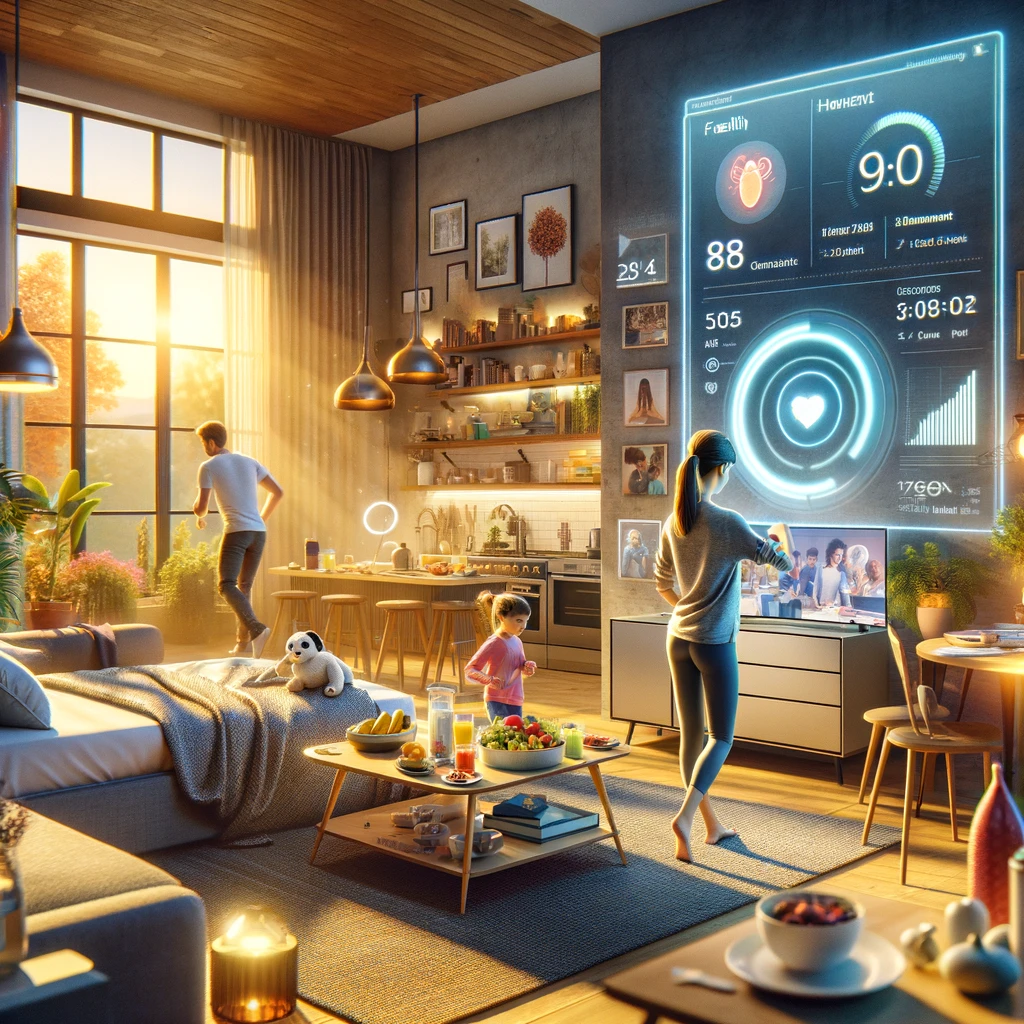
\includegraphics{intro_1.PNG}
	\caption[未来的某个清晨]{未来的某个清晨}
	\label{intro_1}
\end{marginfigure}

早餐后不久,我穿上了智能健身服,这套服装不仅能够监测我的运动数据,还能实时调整锻炼强度,保证我在最佳状态下锻炼。我的智能健身器材根据我的身体状况和健康目标,自动调整了今天的锻炼计划。在运动过程中,智能音乐系统根据我的心率和偏好播放着舒缓的音乐,同时,智能助理还提供心理健康提示,让我的身心同时得到放松和锻炼。

我的孩子们也开始了他们的一天,智能教育系统已经为他们准备好了今日的学习计划。这一系统能够根据他们的学习进度、兴趣爱好推荐适合的学习材料,并通过互动方式让学习变得更加生动有趣。这种个性化的学习方式不仅提高了他们的学习效率,还激发了他们对知识的好奇心。智能家庭教师会实时调整教学内容,确保我的孩子们在最佳的环境中成长。

进入工作状态后,我的智能助理帮我整理了一天的工作日程,并提供了必要的资料和信息。我与我的虚拟团队在虚拟现实空间中开展了会议,利用虚拟现实技术进行头脑风暴和创意讨论。智能家庭教师则帮助我的孩子们在线学习,为他们提供个性化的教育辅导。家庭教育的改变不仅在于学习方式的转变,更在于智能化教育带来的个性化关怀,让每个孩子都能得到最适合他们的教学方式。

工作日的傍晚,我决定去看望父母。我的智能助理不仅即刻规划出了前往父母家的最佳路线,还根据实时交通状况进行了动态调整,确保我能以最快速度到达。我坐进了自动驾驶汽车,它沿着预设路线安静而迅速地穿梭在城市间,将数十公里的距离缩短为仅需的几分钟旅程。

到达父母家时,我通过智能家庭监控系统迅速了解到家中的安全状况及父母的健康情况。这套系统不仅能实时监控家中的安全,还能通过连接的健康监测设备,详细记录并分析父母的健康数据,如心率、血压等重要指标。一旦发现任何异常,系统会立即通知我并提出建议行动,同时智能助手会定期提醒父母按时服药、进行适当的运动,并注意健康饮食,全面保障他们的健康。

回到家中,我被智能家居系统营造的温馨环境所包围。智能灯光根据室内光线自动调整,营造出最舒适的氛围,而智能音乐系统则根据我的心情和偏好播放着轻松愉悦的音乐,让我快速从白天的忙碌中解脱出来,与家人共享宝贵的家庭时光。临睡前,我与我的智能财富管家进行了简短的交流,它根据最新的市场动态为我提供了个性化的理财建议和投资策略,帮助我更好地规划和管理我的财务。

随着智能技术的不断进步,我的生活在各个方面都变得更加智慧和便捷。从健康监测到虚拟现实会议,从个性化学习到创意生产,再到家庭安全和医疗保健,每一项服务都在人工智能的帮助下达到了新的高度。这些技术的融合不仅为我提供了前所未有的便利,也极大地提高了生活的质量和效率。

我深信,在人工智能的引领下,我们将迎来一个更加智慧、美好的未来。这个未来不仅仅是关于技术的进步,更是关于生活方式的革新,让每个人都能享受到更加健康、快乐和安全的生活。随着科技的不断发展,我对未来充满了无限的期待和希望,相信人工智能将继续为我们的生活带来更多的可能性和奇迹。

\section{时光之舞:AI历史交响曲}
\subsection[人工智能概念]{人工智能概念 \sidenote{人工智能是什么、学派有哪些,强人工智能和弱人工智能,人工智能和大脑的关联性}}

人工智能(Artificial Intelligence,简称AI)一词缘于1956年8月美国达特茅斯学院的夏季研讨会。在1955年8月的时候,“人工智能”在一份关于召开国际人工智能会议的提案中被提出,这份提案由东道主约翰·麦卡锡(John McCarthy)、哈佛大学的马文·明斯基(Marvin Minsky)、IBM的纳撒尼尔·罗切斯特(Nathaniel Rochester)、信息论的创始人克劳德·香农(Claude Shannon)联合递交。一年之后,在达特茅斯召开的第一次人工智能大会,而这次会议被认为是开辟了人工智能研究领域的历史性事件,所以一般来说,它的起源要从1956年算起。


人工智能是利用数字计算机或者数字计算机控制的机器模拟、延伸和扩展人的智能,感知环境、获取知识并使用知识获得最佳结果的理论、方法、技术及应用系统。人工智能属于计算机科学的一个分支,研究领域涉及计算机视觉、自然语言处理、搜索与推荐等,同时又与多个学科紧密相关,包括了自动化、电子技术、数学、心理学、语言学、哲学等。

\begin{marginfigure}[-5.5cm]
	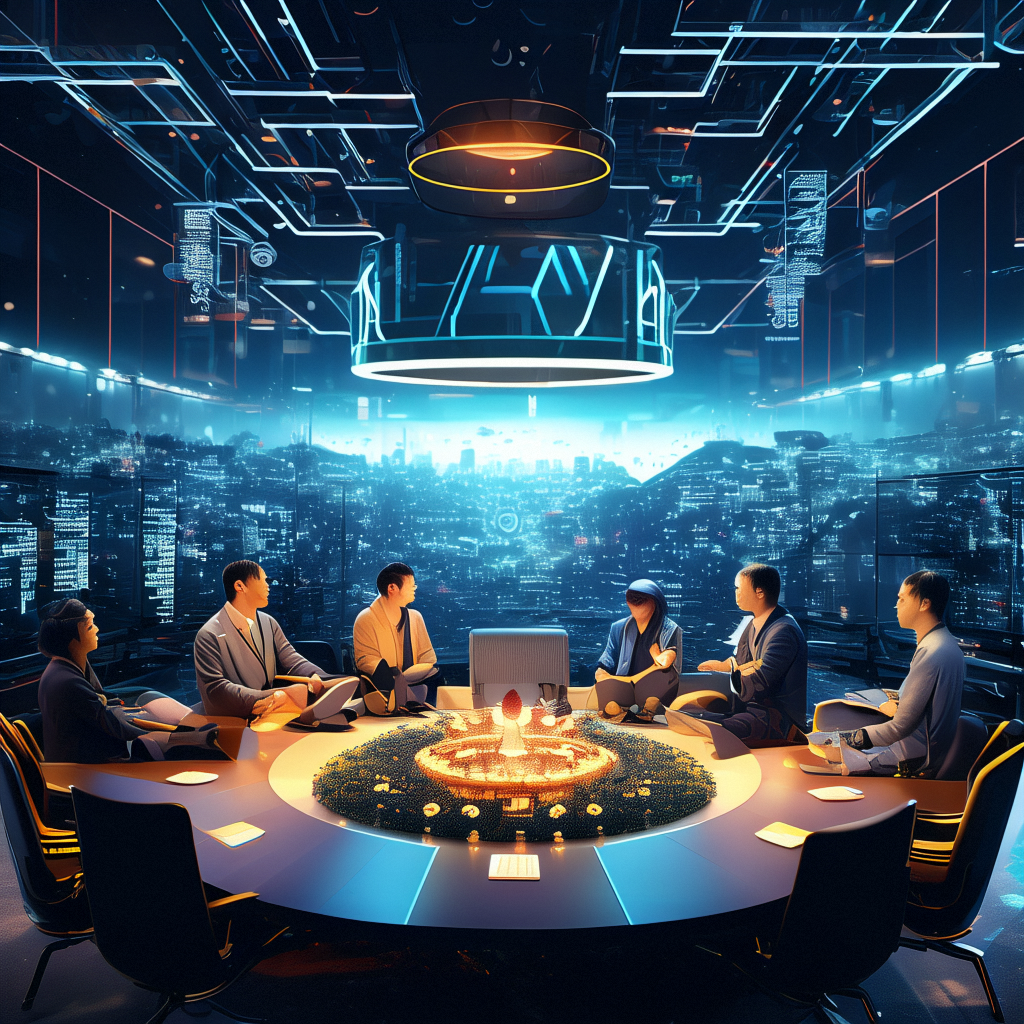
\includegraphics{intro_3.PNG}
\end{marginfigure}

从学术角度来看,人工智能主要包括符号主义、联结主义和行为主义三个学派。其中,符号主义主义的思想起源来自数理逻辑,主张将智能形式化为符号、知识、规则和算法,并用计算机实现符号、知识、规则和算法的表征和计算,从而实现用计算机来模拟人的智能行为,典型的代表算法有决策树;联结主义的思想起源来自衍生学,主张生物智能是由圣经网络产生的,通过人工方式构造神经网络,再训练人工神经网络产生智能,典型的代表算法有神经网络;行为主义的思想起源来自控制论,主张生物智能是自然进化的产物,生物通过与环境及其他生物之间的相互作用,从而发展出越来越强的智能,典型的代表算法有遗传算法和强化学习等。目前,三大学派呈现出逐渐融合的趋势,发挥其各自特点共同持续推动人工智能产业发展。

人工智能可以分为弱人工智能和强人工智能,其中弱人工智能是指不能真正实现推理和解决问题的智能机器,这些机器表面看像是智能的,但是并不真正拥有智能,也不会有自主意识;而强人工智能是指真正能思维的智能机器,并且认为这样的机器是有知觉的和自我意识的,这类机器可分为类人(机器的思考和推理类似人的思维)与非类人(机器产生了和人完全不一样的知觉和意识,使用和人完全不一样的推理方式) 两大类。迄今为止的人工智能系统都还是实现特定功能的专用智能,而不是像人类智能那样能够不断适应复杂的新环境并不断涌现出新的功能,因此都还是弱人工智能。目前的主流研究仍集中于弱人工智能,并取得了显著进步,如语音识别、图像处理和物体分割、机器翻译等方面取得了重大突破,甚至可以接近或超越人类水平。强人工智能不仅在哲学上存在巨大争论(涉及到思维与意识等根本问题的讨论),在技术上的研究也具有极大的挑战性。目前强人工智能鲜有进展,大部分专家任务至少在未来几十年内难以实现。

\subsection[发展历程]{发展历程\sidenote{从国际视角到国内视角,介绍人工智能的主要时间节点}}

人工智能的历史源远流长,许多文明中都有创造人类的神话故事,如西方神话中如赫淮斯托斯的黄金机器人和皮格马利翁的伽拉忒亚,东方神话中的女娲造人等,这些故事反映了是古代人民对于世界和自身存在意义的好奇心和探索欲,是对于存在的深层次思考。现代人工智能的发展不仅是技术进步的体现,更是人类文化和哲学思考的延续。这些古老的神话故事,不仅丰富着我们对人工智能的理解,也指引着我们在技术进步的同时,不忘对人性、生命和存在的反思和尊重。

人工智能的发展从一开始就与计算机科学的发展紧密相连,这种联系可以追溯到计算机科学的早期历史。二战期间,艾伦·图灵的贡献是一个重要的里程碑。图灵不仅帮助英国军方破译了德国军方的著名密码系统Enigma,而且他构造的计算机系统被视为人工智能系统的雏形。图灵的工作展示了计算机不仅可以执行简单的算术运算,还可以进行复杂的逻辑和模式识别任务,这是人工智能的核心能力之一。图灵的贡献还包括他对计算机和人工智能潜力的理论探讨。1948年,他发表的《计算机与智能》论文中提出了著名的“图灵测试”,这是判断机器是否能展现出与人类相似智能的第一个正式标准。图灵测试的提出,不仅推动了人工智能领域的理论研究,也激发了对机器智能可能性的广泛兴趣。图灵的工作不仅为破译代码提供了计算技术,也奠定了现代人工智能研究的基础。他对机器能否思考的探索,以及他开发的技术和理论,都彰显了人工智能作为计算机科学领域内一个长期且核心的研究方向的地方。

人工智能(AI)的历程是一条充满挑战与创新的道路,从理论的萌芽到技术的爆炸式增长,经历了以下六个重要阶段:
\begin{itemize}
    \item 起步发展期(1956年—1960年代初):标志着人工智能概念的正式提出,科学家们在机器定理证明、跳棋程序等领域取得了初步成果,开启了AI研究的首个高潮。
    \item 反思发展期(1960年代—1970年代初):在经历了初期的乐观预期后,更具挑战性的任务揭示了AI技术的局限性,如机器翻译的不足,引发了对AI未来方向的深刻反思。
    \item 应用发展期(1970年代初—1980年代中):专家系统的出现,模拟人类专家解决特定问题的能力,标志着AI从理论走向实际应用的重要突破,尤其在医疗、化学和地质等领域展现了巨大潜力。
    \item 低迷发展期(1980年代中—1990年代中):随着应用的扩大,专家系统的局限性逐渐显现,如知识获取困难、推理方法单一等问题,导致了AI发展的一段低迷期。
    \item 稳步发展期(1990年代中—2010年):网络和互联网技术的飞速发展,特别是IBM深蓝的胜利和“智慧地球”概念的提出,为AI研究注入了新动力,推动技术逐步实用化。
    \item 蓬勃发展期(2011年至今):大数据、云计算等技术的突破,结合深度学习的兴起,极大地推进了AI技术的发展,实现了从理论到实用的巨大跨越,AI技术在图像分类、语音识别等多个领域实现了质的飞跃,迎来了新的高潮。
\end{itemize}

\begin{figure}[htbp]
	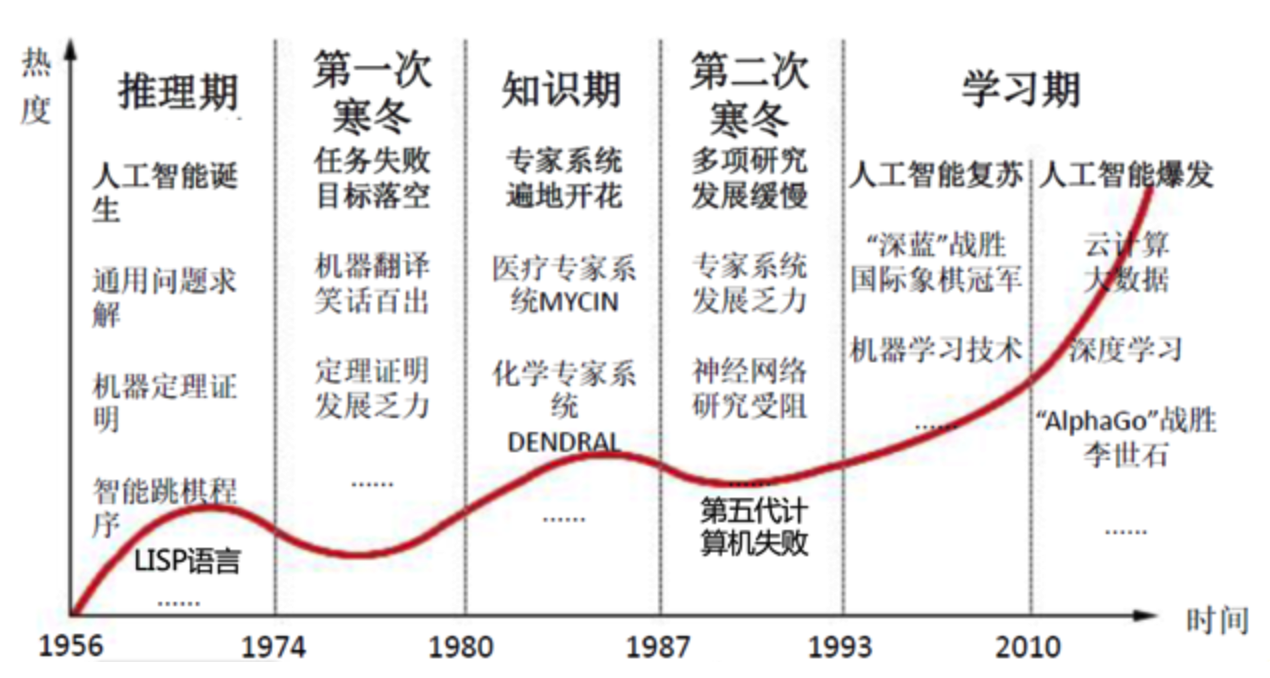
\includegraphics{intro_4.png}
    % \caption[人工智能发展历程]{人工智能发展历程}
	% \labfig{人工智能发展历程}
\end{figure}

人工智能的发展史是科学探索、技术创新与社会需求交织的结果。每一个阶段不仅代表了技术的进步,也反映了在不同历史时期内,人类对于智能本质的理解和追求。从机器定理证明到深度学习,从专家系统到自动驾驶,AI的旅程是对人类智慧的不断挑战和超越,展现了无限的可能性和未来的光明。

今天,人工智能(AI)已经与产业紧密结合,成为推动经济发展和社会进步的关键力量。从智能家居、个性化推荐系统,到自动化生产线、精准医疗,AI的应用遍布我们生活的方方面面,极大地提升了生活质量和工作效率。

AI技术的进步不仅使得设备更加智能,也让服务变得更加贴心和高效。例如,在零售业,通过大数据分析和机器学习,商家能够提供个性化的购物体验,推荐顾客可能感兴趣的商品;在医疗领域,AI能够帮助医生分析病历、诊断疾病,甚至在某些情况下,AI的诊断准确率超过了人类专家。

此外,AI在教育、交通、金融等领域的应用,也正在改变我们的生活方式和工作模式。在线教育平台使用AI来个性化课程内容,适应不同学生的学习速度和风格;智能交通系统能够优化交通流量,减少拥堵;而在金融行业,AI则被用于风险评估、欺诈检测和算法交易等。

尽管AI带来了诸多便利和进步,但它也引发了关于隐私、安全和就业等方面的讨论。随着AI技术的不断发展,如何平衡技术创新与伦理道德的问题,将是我们必须面对的挑战。

\subsection[现状和影响]{现状和影响\sidenote{从国际视角到国内视角,介绍取得的主要成就}}

在过去的六十余年中,人工智能技术经历了显著的演变和进步。特别是在移动互联网、大数据、超级计算、传感网络以及脑科学等领域的新理论和新技术的推动下,人工智能的发展得到了加速。这一时期,由经济和社会发展的强烈需求所驱动,人工智能展现了深度学习、跨界融合、人机协同、群智开放、自主操控等新的发展特征。大数据驱动的知识学习、跨媒体协同处理、人机协同增强智能、群体集成智能、自主智能系统等成为人工智能发展的焦点。受脑科学研究成果的启发,类脑智能正在蓄势待发,而人工智能技术的芯片化、硬件化、平台化趋势更加明显。当前,人工智能的发展已经进入了一个新的阶段,这个阶段特征为新一代人工智能相关学科的发展、理论建模、技术创新以及软硬件的升级等方面的整体推进,引发了链式的突破,并推动了经济社会各领域从数字化、网络化向智能化的加速跃升。

人工智能已成为全球竞争的新焦点。作为引领未来的战略性技术,世界主要发达国家已将人工智能的发展视为提升国家竞争力和维护国家安全的重要战略。这些国家加快出台规划和政策,围绕核心技术、顶尖人才、标准规范等方面强化部署,力图在新一轮的国际科技竞争中掌握主导权。在这一背景下,各国在人工智能领域的投资和研究不断加强,推动了一系列创新和突破,包括自动驾驶汽车、智能家居、智能医疗、机器人技术等领域的快速发展。

面对新形势新需求,为了把握人工智能发展的重大历史机遇,中国的人工智能发展已经被确定为国家战略。中国的最高领导人习近平、李克强对人工智能和机器人学的发展给予了高度的指导和支持。习近平总书记在2014年的讲话中强调了大数据、云计算、移动互联网以及机器人技术的融合发展,以及人工智能领域的迅速进步,这标志着中国对于人工智能及其相关技术的高度评价和对开发这些技术的强烈推动。在这个基础上,中国加大了在人工智能基础研究和应用研究的投资,致力于在人工智能的关键技术和应用领域取得突破,从而在全球人工智能竞争中占据有利地位。

\begin{marginfigure}[-5.5cm]
	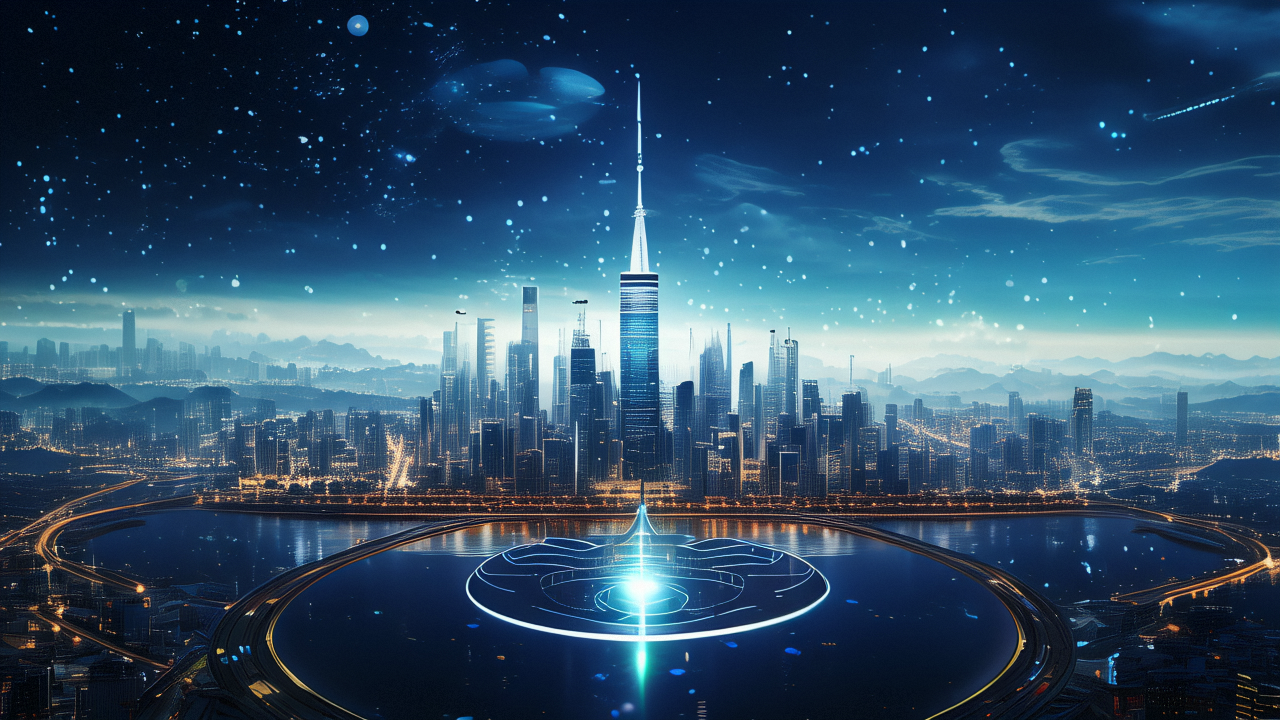
\includegraphics{intro_5.png}
	\caption[中国的人工智能发展已经被确定为国家战略]{中国的人工智能发展已经被确定为国家战略}
\end{marginfigure}

这些年,中国在人工智能领域取得了显著成就,这标志着国家在科技创新和应用实践方面迈出了坚实的步伐。语音和图像识别技术的进步极大地优化了人机交互体验,使得智能助手和面部识别系统更加普及;自然语言处理技术的发展则极大地提高了机器翻译和智能客服的效率和准确性;智能推荐系统的完善为电商、娱乐等行业带来了革命性的变化,使得用户体验更加个性化和高效。

在应用领域,智能制造的推广应用提升了生产效率和质量,降低了制造成本,推动了制造业的转型升级。智能医疗不仅提高了医疗服务的效率和准确性,还通过远程医疗等服务,使得优质医疗资源能够惠及更广泛的人群。智慧城市的构建则在提升城市管理效率、改善居民生活质量等方面发挥了重要作用,通过智能交通系统、环境监测等技术的应用,使城市生活更加便捷、环境更加宜居。

这些技术进步和应用的广泛推广,不仅展现了中国在人工智能领域的强大实力,更在实质上提升了国民的生活质量,并且创造了大量的就业和创业机会。随着人工智能技术的持续发展和深化应用,其在教育、农业、金融等更多领域的潜力将被进一步挖掘,为中国的社会经济发展提供更加广阔的空间和可能性。

这一切的成就,归功于国家对人工智能领域的战略引导和持续投入。通过出台相关政策、增加研发资金支持、构建创新生态系统等措施,中国政府为人工智能技术的研究、开发和应用创造了良好的环境,促进了科技创新与产业发展的紧密结合。这种长远布局和坚定决心,不仅促进了国内人工智能产业的快速成长,也使中国在全球人工智能竞争中占据了有利地位,展现了作为一个崛起中的科技大国的雄心和实力。随着人工智能技术的不断进步和应用的持续深化,预期中国将在推动科技创新和经济社会发展方面实现更多突破,为全球科技进步和人类福祉作出更大贡献。

\subsection[未来和展望]{未来和展望\sidenote{人工智能的未来将何去何从:
- 技术方面,加速大模型的训练和推理
- 应用层面,将人工智能技术和现有产业深度结合,挖掘人工智能技术在更多产业中的应用}}

在过去的许多年,我们见证了人工智能技术的跨越式发展,看到了其在应用层面深度融合现有产业、持续开创新的应用领域的无限可能。随着计算能力的提升、数据量的爆炸式增长以及算法的不断创新,人工智能正在逐步转化为一种基础设施,深刻影响着经济、设计和文化的方方面面。

技术层面上,人工智能的未来将聚焦于加速大模型的训练和推理过程,优化模型效率和可扩展性,同时增强模型的解释性和透明度。通过硬件加速器的创新、新型算法的开发以及云计算和边缘计算的结合使用,未来的人工智能将能够处理更加复杂的任务,实现更高效、更智能的决策和分析。此外,随着人们对于人工智能决策过程的透明度和可解释性要求的提高,提升模型的可解释性将成为重要的研究方向,以确保技术的公平性、安全性和可靠性。

应用层面上,人工智能技术将与各行各业深度结合,推动产业升级和经济结构的优化。在传统行业如制造业、农业、医疗健康等领域,人工智能将通过优化生产流程、提升服务效率和质量、实现个性化需求的满足,来推动这些行业的数字化转型。同时,人工智能也将开辟新的应用领域,如情感计算、虚拟现实、智能交通等,通过这些创新应用,不仅能够改善人们的生活质量,还有助于解决社会、环境等全球性挑战。

随着技术的持续进步和社会的广泛接纳,人工智能的未来充满了无限可能。它不仅会继续推动技术界的革新,更将在更广泛的层面上,促进社会的进步和人类生活方式的转变。面对这样一个充满潜力和挑战的未来,持续的创新、负责任的部署以及跨领域的合作将是推动人工智能健康、可持续发展的关键。

\subsection{问题与反思}
人工智能产业的发展虽然迅猛,但其成长路径上仍面临多项挑战和问题。这些问题不仅关系到技术本身的进步和优化,还涉及伦理、社会和法律等多个维度。以下是一些人工智能产业需要特别关注的问题:
1. 数据隐私和安全:随着人工智能系统对数据的依赖日益增加,如何保护个人隐私和数据安全成为一大挑战。这不仅需要强大的技术解决方案,还需要相应的法律法规和标准来规范数据的收集、使用和分享。
2. 伦理和责任:人工智能的决策过程往往是黑箱的,这引发了关于其决策基础和伦理标准的担忧。如何确保人工智能系统的决策是公正、透明并可解释的,以及在出现错误时如何追究责任,是亟需解决的问题。
3. 技术偏见和公平性:人工智能系统可能会因为训练数据的偏见而产生歧视性的决策,这对于推动社会公平具有潜在的负面影响。确保人工智能系统的公平性和无偏见,要求从数据收集、模型训练到结果评估的全过程进行严格的控制和审核。
4. 就业影响:人工智能技术的发展和应用可能会对劳动市场造成冲击,特别是对于那些重复性高、技能要求低的职业。如何在推进人工智能发展的同时,确保就业机会的公平分配和劳动力的平稳转型,是一个重要议题。
5. 技术壁垒和市场垄断:随着少数大公司在人工智能领域的技术积累和市场控制力增强,存在形成新的技术壁垒和市场垄断的风险。这可能限制创新的空间,增加进入门槛,对整个产业的健康发展构成挑战。
6. 国际合作与竞争:在全球范围内,不同国家和地区在人工智能的发展水平、应用领域和政策制定上存在差异。如何在保护国家安全和促进技术自由交流之间找到平衡,推动国际间的合作而非仅仅是竞争,对于促进全球人工智能产业的健康发展至关重要。

解决这些问题需要政府、产业界、学术界和社会各界的共同努力。通过制定合理的政策和标准、推广伦理指导原则、鼓励开放和透明的技术交流,以及加强国际合作,人工智能产业可以在解决这些挑战的同时,继续保持健康和持续的发展。

\section{结语}

人工智能(AI)技术自1956年提出以来,已经经历了从理论探索到实际应用、从初步发展到技术成熟的演变过程。在技术层面,AI涵盖了符号主义、联结主义和行为主义等多个学派,旨在通过模拟和扩展人类智能,实现机器的自我学习、推理和决策。从弱人工智能到探索强人工智能的旅程中,AI技术已经在语音识别、图像处理、自然语言处理等领域取得了显著进步,且不断向其他领域扩展。

AI的发展受益于计算能力的提升、大数据技术的进步和算法的不断创新,已经成为推动经济、社会和文化深刻变革的关键力量。它不仅优化和改进了现有产业的生产流程和服务模式,而且在医疗健康、智能制造、智慧城市等领域展开了新的应用,极大地提高了效率和生活质量。

然而,AI产业的快速发展也带来了一系列挑战和问题,包括数据隐私和安全、伦理和责任、技术偏见和公平性、就业影响、技术壁垒和市场垄断、国际合作与竞争等方面。这些问题需要通过政府、产业界、学术界和社会各界的共同努力,以及制定合理的政策和标准、推广伦理指导原则、鼓励技术交流和国际合作来共同应对。

展望未来,人工智能将继续在技术和应用层面取得进展,特别是在加速大模型的训练和推理、深化与各行各业的融合等方面。AI的未来不仅在于技术的革新,更在于如何负责任地利用技术,促进社会的公平、安全和可持续发展。随着技术的不断进步和社会认知的深化,人工智能有望为人类带来更加广阔的发展空间和未来可能性。

% \setchapterstyle{kao}
\setchapterimage[6.5cm]{tech_2}
\setchapterpreamble[u]{\margintoc}
\chapter[银幕背后的魔法:人工智能技术]{银幕背后的魔法:人工智能技术\footnotemark[0]}

\footnotetext{The credits for the image above the chapter title go to:
	Image generated by OpenAI's DALL-E, used in accordance with OpenAI's terms and conditions.}

随着ChatGPT模型的爆火,人工智能技术受到社会各界越来越多的关注,大家开始注意到这些应用在不同领域的人工智能算法。人工智能技术的核心是各种各样的算法,但是人工智能算法对于大众来说比较晦涩难懂,需要比较高的数学基础和编程实践能力,而且不同领域的人工智能算法具有比较大的差异,有些算法注重理论,而有些算法则脱胎于工业实践。这加大了人工智能算法的理解难度,也给人工智能技术的介绍带来了一定的困难。为了便于大众的理解,并契合本书的主题,这一章节介绍的人工智能技术的相关算法与实际产业应用和现实生活更加接近。在这一章节,为了激发大家的阅读兴趣,每个章节都会以一些经典或热门电影作为切入点,介绍隐藏在其背后的人工智能技术。

\section{《星际迷航》:语言交融的星际幻梦}

语言是我们日常交流传达信息的载体,历史上不同的国家和民族创造了不同的语言。目前的研究表明,语言的起源与人类进化过程中的社交需求密切相关。随着时间推移和社会变迁,语言也在不断地进行演变,到目前为止,世界上存在着数千种不同的语言,每一种语言都代表了特定文化和群体之间的交流方式,承载着特定文化的价值观、文化传统。另一方面不同的语言也有不同的语法结构和表达形式,这对于不同语言和文化的人之间的交流也造成了一定的困难。

而在《星际迷航:无限太空》中,演员James Doohan首次设计了克林贡语的若干基础词汇及其发音;此后逐渐有越来越多的克林贡语表达在荧幕中出现。之后1985年,美国语言学家Marc Okrand在既有的单个表达的基础上,系统地创制了整套的克林贡语单词和语法,并将之出版在其著作TheKlingon Dictionary中,至此,作为一门完善人造语言的克林贡语的雏形,得以初步确立。在剧中的太空环境下,星舰之间的通信是通过一种名为“次空间通信”的技术实现的。这种通信形式允许以超光速进行数据传输,使得在星际间发送信息成为可能。而人类与瓦肯人之间的语言存在很大差异,造成的交流障碍可以通过人工智能子领域中的自然语言处理来解决。

《星际迷航》中的次空间通信概念可以被视为自然语言处理(NLP)和机器翻译(MT)的高级形式。这些都是人工智能的子领域,专注于通过自然语言实现计算机与人类的交互。目标是使计算机能够以有价值的方式理解、解释和生成人类语言,并实现不同语言之间的互相转换。其中瓦肯人的克林贡语和英语,汉语等人类语言存在较大差距。剧中人物交流使用了一种名为万能翻译器的交流工具,保证说不同语言的人物之间的流畅交谈。

柯克和他的船员经常使用这种万能翻译器,可以立即将外语翻译成人类语言,使他们能够与他们在银河系中遥远星球上遇到的各种外星种族交流。实际上,目前人类并没有发现外星文明,也无法使用万能翻译器翻译外星语言,但是,这种“万能翻译器”其实在现实中已经实现了,谷歌翻译和DeepL翻译器已经实现了大部分语言的即时互译,这种翻译技术是如何实现的呢?接下来本书将从历史发展,技术原理等方面介绍机器翻译技术。

\subsection{翻译的起源}
在古代,由于交通不便,文明之间的交流比较少,一般是由边境杂居通晓两种语言的人担任翻译;在交战或和谈时,国家选派的外交使臣一般也可以作为翻译官。然而这种翻译效率较为低下,无法很好地完成信息传递。随着技术的进步,计算机被科学家制作出来,紧接着在1954年乔治城大学的科学家们成功将60多条俄文句子翻译成英文,标志着机器翻译的开始。虽然当时这些句子是经过实验人员精心挑选的,但依然展示了计算机在语言翻译方面的潜质。后来,学者们经过不断钻研,提出了各种各样的翻译方法,使得机器翻译技术的效果越来越好,接下来本书会按照方法特点以及提出先后分三阶段进行介绍。

\subsection{基于规则与实例的机器翻译}
第一阶段是基于规则的技术,每种语言都有自己的语言范式,我们需要理解语言的含义才能做好翻译。通过对语言结构和句法规则的理解,翻译员才能够将陌生语言的含义正确地表达出来,但这引出了一个问题,如何能够通过较低的代价深入地分析语言的共同特性?众所周知,人类的本质是复读机,自然而然地人们想到通过借鉴实例的方式进行翻译,但语言是复杂的,实例数量过于巨大,检索过程会很耗时;而且一些新词汇或陌生的语言会遇到检索不到的问题,所以这种方法现实不可行。

那要怎么办呢?既然语言都有底层的逻辑和规则,我们就可以找语言学家制定规则,翻译的时候根据规则操作就可以更加流畅地进行翻译了,那这些规则包含哪些要素呢?一般来说,规则会包含用法和词典两部分,以中英文为例,词典是英文单词与中文汉字的对应(“我”:“me”(宾语),“I”(主语)),用法是句法结构的对应(汉语主谓宾→英语主谓宾)。一个规则系统通常会包含上万条基本词典、领域词典以及人名地名词典;数千条句法规则和生成规则;并给出数万条翻译实例。制定规则的过程需要深入理解两种语言的内在结构和特点,同时也需要考虑到语言的灵活性和变化性。因此,这通常需要语言学家、翻译专家和计算机科学家的共同努力。但规则又会面临以下的问题:出现新的词语,需要扩大词典;出现新的规则,需要加入规则的同时保证不与原始规则冲突,这些更新都需要专家进行,维护难度会很大。

\subsection{统计机器学习}

随着数据资源越来越丰富,计算能力越来越强,学者们尝试新的思路进行机器翻译。既然数据资源变得越来越丰富,那么我们可以收集数据,对数据中的规律进行总结,并根据总结的规律进行翻译,于是统计机器翻译应运而生。统计机器翻译的基本流程包括以下几个步骤:第一步:预处理,将源语言和目标语言的语料库进行预处理,包括分词、词性标注等。第二步:词对齐,构建源语言和目标语言之间的词汇对应关系矩阵,以及句子之间的翻译概率矩阵。第三步:模型训练,基于构建的矩阵,使用统计方法训练机器翻译模型。第四步:翻译生成,给定一个待翻译的源语言句子,利用训练好的模型生成目标语言的翻译。

统计机器学习的核心是概率模型的选择和优化。落到机器翻译领域,统计机器翻译主要使用短语对齐模型和基于短语的统计机器翻译模型。短语对齐模型通过分析源语言和目标语言之间的词汇对应关系,找出短语级别的翻译对应关系。基于短语的统计机器翻译模型则在此基础上,通过最大熵模型或者条件随机场模型,学习出短语之间的翻译概率,其中概率模型句子的生成采用训练数据上的极大似然估计,选取概率最大的词语组成翻译。但该方法流程比较复杂,翻译性能遇到瓶颈后很难大幅度提升。


\subsection{神经网络机器翻译}

随着深度学习技术的发展以及数据资源的进一步丰富,能够支持数据表示从符号表示转化为连续表示,机器翻译进入了下一阶段,这一阶段通常被称为神经网络机器翻译,与传统的统计机器翻译相比,神经网络机器翻译具有更好的翻译质量和更高的翻译效率。由于翻译涉及两种语言之间的转化,因此一般使用的架构是编码器-解码器架构。

编码器将源语言句子的每个单词或字符映射到一个向量空间中,这些向量表示了单词或字符的语义和语法信息。然后,编码器将这些向量组合成一个固定长度的向量,这个向量被称为编码向量。编码向量包含了源语言句子的全部信息,是解码器生成目标语言翻译的基础。

解码器则根据编码向量生成目标语言的翻译。解码器通常是一个循环神经网络,它将编码向量作为初始状态,并通过循环计算生成目标语言的每个单词或字符。在每个时间步,解码器都会生成一个单词或字符,并将生成的单词或字符和编码向量作为输入,进行下一步的循环计算。
为了提高翻译质量,神经网络机器翻译通常还需要引入注意力机制。注意力机制允许解码器在生成每个单词或字符时,根据源语言句子的不同部分来加权编码向量。这样做的好处是句子中的单词之间通常存在联系,注意力层可以隐式地学习到这种联系,从而让翻译结果更加地通顺与合理。

总的来说,神经网络机器翻译是一种比较先进的机器翻译方法,它通过神经网络和注意力机制,实现了从源语言到目标语言的高效、准确的翻译。随着深度学习技术的进一步发展,神经网络机器翻译的性能将会得到更大的提升。

\section{《头号玩家》:视觉之幻}
《头号玩家》中的虚拟现实世界是一座名为“绿洲”(OASIS)的庞大虚拟宇宙,由天才设计师詹姆斯·哈利迪创建,这部电影也是非常经典的科幻作品,其中的“绿洲”应用了虚拟现实技术、计算机视觉(CV)技术以及其他先进技术。

\subsection{面部识别技术}

想要玩家的虚拟化身准确地反映玩家现实中的脸部表情和动作需要使用先进的面部识别技术,而且面部识别技术可以也可以确认用户身份,防止非法用户进入“绿洲”。而现实中的面部识别技术与电影中展现的技术类似,这一小节让我们来了解一下它的发展与应用。

面部识别技术是一种基于计算机视觉和模式识别技术的人脸检测和识别技术。它可以检测、识别和验证一个人的面部特征,有身份验证、安全监控、支付验证等多种用途。面部识别技术的起源可以追溯到20世纪60年代,当时采用的方案也是很朴素的数学几何特征,这集中体现在学者们对于剪影的研究上,人们对面部剪影曲线的结构特征提取与分析方面进行了大量研究,但没有收到很好的效果,也基本没有落地的应用。

突破发生在上世纪90年代,诞生了一些典型的识别技术,并产生了军事应用技术。美国麻省理工学院媒体实验室的特克和潘特兰德提出的“特征脸”方法是一种基础的人脸识别方法,之后的算法或多或少收到了该方法的影响。例如同一时期的“Fisherface”方法就有“特征脸”的思想,对输入的人脸图像进行主成分分析,提出脸部特征,然后再使用其他的算法将不同人脸的特征区分出来,达到人脸识别的效果。这一时期美国军方组织了著名的FERET人脸识别算法测试,并出现了若干商业化运作的人脸识别系统,比如最为著名的Visionics的FaceIt系统。这一时期面部识别技术蓬勃发展,不仅出现了影响后世的算法,还成功地实现了商业转化。

但这些算法会受到光照,拍到的面部表情,姿势等非理想的图片采集状态的影响,随着进入新世纪,机器学习模型的发展,支持向量机,弱分类器组合以及神经网络技术被应用于面部识别应用场景中,缓解了由于图片采集造成的识别不准确问题。近年来,随着深度学习技术的发展,面部识别技术也取得了显著的进步。深度学习技术可以提取更加丰富的面部特征,并通过神经网络进行特征匹配,从而提高面部识别的准确性和鲁棒性。目前,深度学习技术已经成为了面部识别技术的主流方法。目前卷积神经网络是面部识别技术使用最多的算法,它的主要优势是可用大量数据来训练,从而学到对训练数据中出现的变化情况稳健的人脸表征,而且不需要设计对不同类型的类内差异的特定特征。

\subsection{动作捕捉技术}

“绿洲”中虚拟角色的运动可能使用了动作捕捉技术(以下简称动捕)来模拟现实中玩家的具体动作,从而增强真实感。同样地在现代电影的拍摄过程中,动捕也是一项非常重要的辅助技术。但从宽泛的角度出发,动捕是一个非常通用的概念,它的目标可以是人体运动、面部表情、物体运动以及个体的局部信息等。动捕的起源很久远,最早是动画师发明的动作转描技术,代表作有迪士尼1937年的《白雪公主与七个小矮人》,以及1941年的《铁扇公主》和1958年的《白蛇传》。从1980年代开始,机器类的动捕设备(穿戴式)开始研发并投入使用,任天堂和麻省理工也提出了各自的光学动捕系统。

近年来,随着计算机视觉技术的发展,动作捕捉技术也取得了显著的进步,例如可以利用深度学习技术来提高动作捕捉的准确性,并将其应用于游戏开发、虚拟现实等场景。此外,动作捕捉技术也可以应用于机器人控制,以实现机器人的自主运动。国内也不乏高质量的动作捕捉系统,像诺亦腾、自然动点、青瞳视觉还有国承万通等等。另外,这几年虚拟主播的崛起使得动捕技术的应用变得更加的广泛,结合动作与面部表情的生成,主播的虚拟形象正在变得越来越精致。

\subsection{拓展现实技术}
在电影《头号玩家》中,拓展现实技术主要体现在虚拟现实(Virtual Reality, VR)和增强现实(Augmented Reality, AR)的应用上,这两种技术共同构成了电影中的“绿洲”(OASIS)世界。

虚拟现实技术在电影中表现为:人们通过佩戴高级的VR头盔(OASIS头盔)和全身跟踪设备,完全沉浸在绿洲这个虚拟世界中。他们可以在绿洲里自由移动,体验各种场景,如游戏、冒险、社交等。而通过游戏冒险等开放式挑战,绿洲将平时在电脑或手机中的游戏拓展到一个近似现实的空间中,玩家能够沉浸式体验各种冒险挑战。另一方面,虚拟环境也提供了虚拟社交平台,玩家可以在虚拟环境中与其他玩家互动,包括聊天、组队、深层次的友谊,甚至结成虚拟伴侣。此外,在类似绿洲的虚拟环境中,玩家也可以进行虚拟形象设计,发挥各自想象力,创造出千奇百怪的虚拟人物形象,甚至定制外观和能力,以展现玩家的个性。

而增强现实技术表现在现实生活中虚拟形象的投影,电影中的韦德在与虚拟角色进行对话时,利用增强现实技术可以在现实中展现角色的形象,使双方交流更有真实感。而在某些场景的虚拟现实设备启动时,韦德需要增强现实设备进行控制,比如使用类似智能手机的设备启动VR眼镜等设备,体现了增强现实技术在交互过程中的应用。

这些拓展现实技术的起源能够追溯到上个世纪60年代,其中1968年,Ivan Sutherland和他的学生Bob Sproull开发了头戴式显示器(达摩克利斯之剑),被认为是第一款现实中的AR/VR设备。上世纪80年代,3D眼镜被发明出来,并由StereoGraphics公司进行了生产,但直到本世纪,3D眼镜才逐渐流行开来。而拓展现实技术真正进入大众视野是在20世纪90年代,这一时期虚拟现实游戏机,VR眼镜,家庭VR设备陆续被各大公司创造出来,使拓展现实技术实现家庭或个人应用成为可能。而同期军事和工业领域也开始应用VR技术进行模拟实验,拓展了虚拟现实技术的应用空间。

本世纪初,随着移动设备的普及和计算能力的提升,AR技术开始逐渐被应用到手机APP中,如谷歌眼镜就是这一时期的代表。2016年,随着Pokemon Go的全球流行,AR技术进一步走进公众视野。VR技术也在这一时期获得了显著发展,代表设备有Oculus Rift、HTC Vive和PlayStation VR等。近年来,随着5G网络、AI、云计算等技术的发展,拓展现实技术正在加速走入日常生活,应用涵盖教育、医疗、工业、娱乐各个领域。未来,随着技术的不断进步,拓展现实技术有望带来更多的创新应用和体验。

虽然拓展现实技术如此的美好,但也有一些潜在的隐患。当虚拟现实能够以假乱真的时候,我们真的能够分辨出自己所处的地方到底是现实的还是虚拟的吗?游戏中的生活再美好终究也是虚假的,游戏中的你再强大,依然改变不了现实中“人被杀就会死”的真理。正如电影中的主角那样,在完成终极任务后,他终于找到了真正的自我,感悟到世间的真实情感,意识到“绿洲”不是逃避糟糕现实的避难所,面对挫折不能一味逃避而要勇于面对。最后,韦德在掌管了“绿洲”所有权后宣布,每个星期将有两天关闭“绿洲”,鼓励人们更多地体验和感受真实的生活。技术是为人类服务的,我们需要有正确的认识,并合理地使用这些技术,才能让真实的生活更加美好。

\section{《钢铁侠》:音声的魔法}

贾维斯作为托尼的得力AI助手,在电影中给观众留下了很深的印象。虽然它的名字原意为”只是一个相当聪明的智能系统“,但显然这个智能系统会的技能有点太多了。它的能力包括但不限于连接到任意计算机终端;操控斯塔克的房屋和钢铁侠战服的内部系统;与托尼进行交谈以及开车等等。贾维斯其实代表了一种高度智能的语音识别和交互技术,将电影中的科技元素推向了新的高度。那么贾维斯具体包含了哪些人工智能技术呢?下面就为大家一一介绍。

\subsection{语音识别技术}

在电影中该技术具体表现为:贾维斯能够准确识别托尼的语音命令,无论是简单的指令,还是复杂的计算机操作,它都能迅速理解和执行。而现实中存在的语音识别技术需要我们输入音频(语音或对话),然后模型生成对应的文字信息。然而,我们人类经历了几百万年的进化才形成了丰富的语言系统,而且需要后天的学习才能真正掌握发音和语法,从而听懂他人的话语,表达自己的观点。那么像贾维斯这样的AI系统是如何识别我们人类的语音呢?接下来,让我们从语音识别技术的起源讲起,了解这一技术近百年的发展历史吧。

回顾语音识别技术的历史,其起源可追溯到20世纪50年代,那时的科学家致力于探索如何将口头语言转化为计算机能够处理的文本形式。此时,美国的贝尔实验室已经开始研究语音识别技术。到了60年代,贝尔实验室开发了一个名为“AUDREY”的语音识别系统,该系统可以识别数字和简单的单词。这个系统使用了手工设计的规则来匹配语音特征和词汇,然而该系统对特定人的声音特别依赖,难以适应不同的说话人的语音。随着技术的进步,70年代第一代语音识别系统开始出现,这些系统主要使用了规则引擎和手工设计的特征提取方法来实现语音识别,但这样的系统准确率相对较低,且无法识别不同的语音特征和语言,具有很大的局限性。

到了1980年代,隐马尔可夫模型(HMM)被引入到语音识别中,大大提高了识别的准确性,使得系统能够识别更复杂的词汇和短语。尽管这些系统在特定词汇集上的表现有所提升,但对连续语音和自然语言的理解能力仍然有限。1990年代,随着大规模语料库的收集和计算能力的提升,语音识别技术开始进入实用阶段。微软的“Microsoft SAPI”是这一时期的代表,win95支持该模块的运行,而且在90年代,微软一共推出了SAPI 1-4一共4个版本的API,升级了对口语以及不同程序语言的支持,应用场景也变得越来越广。

本世纪初,随着数据量的增加,深度神经网络(DNN)开始被应用于语音识别,极大地改善了识别效果。深度学习的引入使得系统能够自动从大量数据中学习特征,从而能够适应不同人的音色以及不同的语言,这是一个巨大的飞跃。研究者如Geoffrey Hinton和他在多伦多大学的团队推动了深度学习在语音识别中的应用。2011年,IBM的“Watson”在电视问答节目“危险边缘”中击败了人类选手,展示了深度学习在理解自然语言和语音识别上的潜力。谷歌、微软、亚马逊等科技巨头也纷纷推出基于深度学习的语音识别服务,如谷歌的“Google Speech API”和亚马逊的“Amazon Transcribe”。

近年来,随着硬件和云计算的快速发展,语音识别技术已经广泛应用于智能手机的语音助手、智能家居、自动驾驶汽车和医疗诊断等领域。未来,随着人工智能的进一步发展,语音识别将更加智能化,能够更好地理解语境、情感和意图,为人类带来更为便捷的交互体验。

\subsection{语音合成技术}

与语音识别技术相对应的是语音生成技术,虽然电影中的贾维斯可以聘请配音演员进行配音,但现实中的AI对话不可能找演员进行实时配音。此时我们需要一个可以生成语音的模型帮助我们生成需要的声音,一般情况下,此类模型需要的输入为声音对应的文本数据,可以是简单的单词、句子、段落或完整的文档,在应用的时候可以是用户输入的命令、文章内容、电子书文本等;另外,有些模型也可以输入一些要求,比如:语气的轻重缓急,重音位置,声音性别等个性化需求。对应的输出一般为音频流,有实时的语音信号或者保存为MP3,WAV等格式的音频文件,以便用户的存储和播放需求。从这个角度来说,语音合成技术通过将文本转换为可听的语音,实现了信息的无障碍传递,为视觉障碍人士、语言障碍人士以及有阅读困难的人提供了极大的帮助。

而语音合成技术的起步甚至比语音识别技术更早,在1930年代,科学家开始探索通过机械和电子设备生成语音的可能性,但并没有什么实质性的成果。到了1962年,有实验室展示了他们发明的可以合成语音的机器,但这时是实验人员调整机器参数,生成的声音极其有限。之后到了70,80年代,根据声学底层原理提出的一类共振峰合成器成为了主流的语音合成技术,只要实验人员精心调整参数,此类合成器能合成出非常自然的语音。而最具代表性的文语转换系统数美国DEC公司在1987年提出的DECtalk,该系统采用Klatt的串/并联共振峰合成器,可以通过标准的接口和计算机联网或单独接到电话线路上提供各种语音信息服务,它的发音清晰,并可产生几种不同音色的声音,供用户选择。

八十年代末期,语言合成技术又有了新的进展,特别是1990年研究员们提出的基音同步叠加(PSOLA)方法,该方法采用时域波形拼接的思想,使得合成的语音的音色和自然度大大提高。之后,不同语言的PSOLA方法也陆续被科学家们实现,基于这类简单的方法,可以开发出很多语音合成系统,比如中国科学院声学所的KX-PSOLA(1993),联想佳音(1995)。但这些系统合成的句子及篇章语音机器味较浓,其自然度还不能达到用户可广泛接受的程度,从而制约了这项技术的大规模进入市场。

21世纪以来,随着统计建模和机器学习算法的发展,语音合成技术开始采用隐马尔可夫模型(HMM)和波形建模等技术,使语音合成的自然度显著提高。这一时期的代表是IBM开发的可以在嵌入式设备中使用的Viavoice,该系统由6个部分组成,不仅提供了语音合成功能,也可以进行语音识别。

\subsection{情感理解技术}

该技术属于心理学和计算机科学的交叉领域,电影中的贾维斯能够理解托尼的情感,直到它“死亡”都没有背叛过托尼,具有鲜明的人物形象。但现实中该能力对AI来说是一项很有挑战性的任务,从这一技术的历史发展我们可以感受到这一技术挑战的难度。

情感理解的提出在上世纪80年代左右,当时科学家做的是情感识别工作,例如通过使用规则或统计模型分析文本中的情感词汇和语调来识别作者的情绪,显然这项任务与情感理解具有很大的差异。90年代后,研究人员开始构建情感词典,通过量化含有情感的词语的方式进行情感识别。到本世纪,科学家们又引入机器学习方法和深度学习模型进行文本情感的理解。最近十年,随着生成式模型的出现,情感反馈与生成也成为了该领域的研究热点,该任务不仅要求模型能够识别情感,还需要生成具有情感色彩的回复。

但这也产生了一个问题,AI模型是否具备自我意识,是否存在伦理与法律上的问题。虽然目前AI模型已经很大,可以完成各种各样的任务,但它们还不具备真正的自我意识。然而随着科技发展,未来的人工智能是否会拥有自我意识仍然是一个未知的事情。

\section{《流浪地球》:大模型的奇幻时代}
\subsection{科幻作品中的大模型}

在电影《流浪地球》中,MOSS是一个智能量子计算机,后因“隔离计划”被转移至领航员空间站,负责管理空间站事务,是“流浪地球”计划辅助执行者、“火种”计划的执行者,拥有联合政府授权。其拥有两种形态,其中生活仓的MOSS为白色,在总控室的MOSS是黑色。虽然在电影中MOSS算是辅助角色,但其具备的能力确实十分的强大,具有丰富的世界知识,能够进行自主学习并适应环境变化,可以进行自主决策并与主角进行流畅的对话。

虽然MOSS十分强大,但目前现实中并没有类似的AI模型拥有与之匹配的能力,如果矮子里面调将军的话,大模型算是最接近MOSS的人工智能技术。那么,什么是大模型呢?

\subsection{大模型技术介绍}

大模型目前没有一个非常明确的定义,通常指人工智能领域中,拥有海量参数的复杂模型。这些模型通常用于处理自然语言处理(NLP)、图像识别、语音识别等多种任务,能够从大量的训练数据中学习到复杂的模式和特征。大模型一般情况下使用神经网络架构(Transformer),其参数量一般可以达到十几亿甚至数千亿,这使得它们有能力学习更为精细的数据特征,并能更好地适应各种复杂的任务。由于大模型的参数量巨大,模型训练时需要的数据量也很大,而且大模型通常采用预训练的方式,通常先在一个大规模无标注的数据集上进行预训练,学习通用的语言或视觉表示。该数据集一般是收集网络上的数据后进行筛选构成的,训练时,这些数据(很多都是类似对话、文章等长序列数据)被输入给模型,随后转为词向量进行进一步的特征提取,最终大模型学到这些数据的通用表示。之后,可以根据特定任务需求在相关的小数据集上进行模型微调,以提升在特定下游任务上的性能。目前,训练大模型需要大量的计算资源,包括高性能的GPU或TPU等硬件,以及海量的数据和模型的存储空间。不过同时,大模型在自然语言理解和生成、智能助手、自动翻译、推荐系统等领域具有广泛的应用。

\subsection{大模型的发展历史}
大模型相关技术的提出还是比较早的,上世纪50年代神经网络已经被学者们提出并进行了实验,但当时由于组成神经元的参数过少,数据量不足等原因,神经网络的效果比不过专家系统和规则方法。因此神经网络方法沉寂了约40年的时间,直到1980年代,卷积神经网络(CNN)的雏形出现,为图像识别和计算机视觉领域带来了新的突破,之后在1990年代末,现代CNN的基本结构LeNet-5被提出,深度学习技术开始崭露头角。

随着自然语言处理技术的发展,词向量模型被提出,标志着大模型的部分底层技术逐渐成形。2017年,Google提出了Transformer模型,该模型以其自注意力机制和并行处理能力,为处理长序列数据提供了新的方法。2018年,GPT-1和BERT模型的发布,开启了预训练模型的时代。

随着技术的积累和数据量的增加,模型参数量变得越来越大,2020年,OpenAI的GPT-3(Generator Pre-training-3)模型横空出世,拥有1750亿参数,成为当时最大的语言模型。此时,模型的参数规模达到了前所未有的水平,为零样本学习(可以理解为没有模型微调阶段)和自然语言处理带来了巨大进步。同时研究人员在训练GPT-3时也使用了一些新提出的技术,如基于人类反馈的强化学习(RLHF)和代码(编程语言)预训练。

等会,我们介绍了那么多,怎么还没有大模型这一概念呢?事实上,大模型这一概念是很多人工智能技术综合的产物,直到22年底OpenAI提出ChatGPT模型并引发广泛关注,通常意义上的大模型才出现在大众的视野,由于模型参数量变得很大,这一类的模型被称为“大模型”,其自然语言交互能力在多个领域展现了巨大潜力。另一方面,随着视觉-语言模型如CLIP(Contrastive Language-Image Pretraining)和DALL-E的推出,研究人员开始整合视觉和语言信息,并提出可以处理多类输入信息的大模型。

在国内,产业界、投资界和研究机构等都在投身大模型研究。首先,国内科技龙头企业纷纷发布自主研发的大模型,比如百度推出了大模型文心一言,阿里巴巴发布了大规模语言模型通义千问,智谱AI也率先进行了商业化的落地,推出了不同参数量级的商业化模型ChatGLM系列。这些竞争促进了大模型社区的良性发展,目前世界范围内呈现出“百模齐放”的景象,出现了兼容不同语言,不同模态的大模型。

大模型的发展不仅推动了人工智能技术的进步,也在实际应用中产生了深远影响,如智能助手、自动翻译、推荐系统等。目前,研究人员也在积极探索大模型在生物医学,化学制造等方面的应用,包括但不限于制造化学分子,进行化学实验,模拟生成人工蛋白质等。


\pagelayout{wide} % No margins
\addpart{产业篇:智慧蔓延}
\pagelayout{margin} % Restore margins
% \setchapterstyle{kao}
\setchapterpreamble[u]{\margintoc}
\chapter{机械幻想和智慧工厂:工业4.0}

创新是引领发展的第一动力。2013年德国政府提出“工业4.0”战略,并在当年的汉诺威工业博览会上正式推出。工业4.0指利用人工智能技术,由集中式控制向分散式增强型控制的基本模式转变,目标是建立一个高度灵活的个性化和数字化的产品与服务的生产模式。主要分为智能工厂,智能生产,智能物流三大主题。自提出以来,工业4.0迅速成为德国的另一个标签,并在全球范围内引发了新一轮的工业转型竞赛。

人工智能智慧工厂是工业4.0的核心主题之一。智慧工厂是指利用人工智能技术,辅助以大数据分析,多模态感知等先进技术手段,将传统工厂严重依赖于人工监督的流水线转变为智能化、自动化、高度灵活的生产方式。智慧工厂依赖于传感器、机器人、自动化设备和互联网等技术,实现生产过程的自动化控制、智能优化和数据驱动决策。在人工智能智慧工厂中,各种设备和系统可以相互连接和通信,形成一个智能化的生产网络。传感器和物联网技术能够实时收集和传输大量的生产数据,而人工智能算法则能够对这些数据进行分析和解读,从中提取有价值的信息。这些信息可以用于优化生产计划、预测设备故障、改进产品设计等方面,从而提高生产效率和产品质量。

如果说智能工厂改变了传统生产加工方式的执行者,那么智能生产则是统筹规划工业进程的指挥者。智能生产主要涉及整个企业的生产物流管理、人机互动以及3D技术在工业生产过程中的应用等。该计划将特别注重吸引中小企业参与,力图使中小企业成为新一代智能化生产技术的使用者和受益者,同时也成为先进工业生产技术的创造者和供应者。智能生产的概念涵盖了从生产计划、物料采购、生产过程监控到产品质量管理等方方面面,旨在构建一个高效、智能和可持续的工业生产体系。

智能物流是工业4.0的另一个主题。智能物流主要通过互联网、物联网、物流网,整合物流资源,充分发挥现有物流资源供应方的效率,而需求方,则能够快速获得服务匹配,得到物流支持。得益于我国巨大的消费市场,物流行业在我国有着广阔的发展前景。早在2008年,全国社会物流总额达89.9万亿元,比2000年增长4.2倍,年均增长23\%,较欧美发大国间同期领先200\%。中国物流与采购联合会发布的2023年物流运行情况分析指出,2023年全国社会物流总额为352.4万亿元,按可比价格计算,同比增长5.2\%,增速比2022年提高1.8个百分点,仍然占据着全球前列。我国在物流的智能化道路上同样进展喜人,2019年,京东物流在北京“亚洲一号”建设并落成国内首个5G智能物流示范园区,它实现了5G 网络通信与物流应用的深度融合创新,带来了智能物流园区的数字化与智能化。目前,我国坐拥成熟的快递物流系统,实现了物流的数字化管控,在智能物流方面处于世界领先水平。

自工业4.0提出以来,各国都开始了各自的工业改革道路,全球范围内展开了新一轮的工业转型竞赛。近年来,我国互联网企业发展迅速,人工智能技术在行业内应用逐渐成熟,已经为再一次产业升级打下了坚实的基础。我国政府对工业4.0保持了高度重视,早在2014年,我国就和德国签署了《中德合作行动纲要》。时任总理李克强表示:我国要在工业化与信息化同步发展的战略中更快地促进两者的融合。2015年,我国提出了《中国制造2025》的发展纲要,明确指出工业发展三步走的战略目标,即:到2025年,我国装备制造业进入世界装备制造强国第二方阵,部分优势产业率先实现又大又强;到2035年,我国装备制造业位居世界第二方阵前列,成为名副其实的装备制造业强国;到2045年,我国装备制造业进入世界装备制造强国第一方阵,成为具有全球影响力的装备制造业强国。2016年以来,诸多工业4.0相关政策陆续出台,包括《智能制造发展规划(2016-2020年)》、《智能制造工程实施指南(2016-2020年)》、《工业互联网创新发展行动计划(2021-2023年)等重磅政策陆续出台,从政策层面给予工业4.0重要的支持,更明确了我国工业4.0的发展目标及策略。与此同时,德国、日本、美国等制造业强国也都提出了各自的工业发展规划。可以预见的是,未来20到40年内,第四次工业革命将改变目前的生产生活方式,并且极大的影响着世界发展格局。

\section{机器人技术:AI赋予机器自主行动能力}
\subsection{从“机器”到“人”,ai赋予机器新活力}

以机器代人工作的思想起源于文明发展初期,传闻春秋时期的工匠鲁班利用竹子和木料制造出一个木鸟,它能在空中飞行,“三日不下”,这件事在古书《墨经》中有所记载,可见人们对能够解放人类双手的生产方式渴望已久。1920年,捷克斯洛伐克剧作家卡雷尔·凯培克在他的科幻情节剧《罗萨姆的万能机器人》中,第一次提出了“机器人” (Robot)这个名词,被认为是机器人一词的起源。在捷克语中,Robot这个词是指一个服役的奴隶。这也是现在我们对机器人的一般理解,即能够帮助人类完成指定任务的机器。

通常将机器人发展历程分为三个阶段。第一阶段是可编程机器人,这类机器人通过人工编写的特定执行命令,不能根据环境调整自身行为,只能完成一些简单的重复劳作。第二阶段在可编程机器人的基础上添加了传感器,即自适应机器人。第二代机器人具有不同程度的感知能力,能够根据环境中特定指标的变化改变策略,目前大量应用于工业生产中。第三代机器人通过内置的人工智能程序进行调度,具有识别、推理、规划和学习等智能机制,它可以把感知和行动智能化结合起来,因此能在非特定的环境下作业,故称之为智能机器人。

人工智能技术使得机器人真正跳出了预设的框架,迈向了智能化,自主化的新阶段。下面我们来介绍人工智能用于机器人的几个关键技术。

感知与认知技术是人工智能机器人的关键技术之一。以各类传感器为基础,感知技术为机器人提供了观测实际环境的能力。机器人可以从环境中获取各种传感器数据,如视觉、声音、温度、磁场等信息,并立即进行处理和分析,转化为机器人能够理解的数据流。随后,以数据挖掘,深度学习,强化学习等智能算法为核心的认知技术对感知得来的数据进行理解和解释,通过学习和推理来做出智能决策和行为。要将感知学习与认知科学结合起来并非易事,如何面对复杂多变的真实情况是机器人技术难以绕开的问题。为此,研究人员搜集整理了大量实际生产中的数据,包括各种情况下恰当的做法,这部分也称为“记忆”,用于训练模型,由此来理解和推理实体物质。在构造好适宜的数据后,深度学习和强化学习彼此构建,形成了一种强有力的人工智能开发方式。深度学习能够处理各类型的数据,允许计算机解决更加复杂深奥的任务,包括视频、图片理解和语音处理等;而强化学习模仿了人类的学习过程,引进了奖励/惩罚机制对机器人的每个动作进行评估,从而引导机器人做出正确决策,获得长期收益。目前,感知与认知技术已经在自动导航,故障监测,智能控制等方面得到广发运用,并取得巨大的成功。

人机交互与自然语言处理技术是增强人机沟通和互动的重要技术。通过设计用户友好的界面和自然易懂的交互方式,如语言指令、手势识别和面部表情识别,人与机器人之间可以进行高效、透明的交流。自然语言处理技术旨在研究人类和机器之间用自然语言进行有效通信的理论和方法。自然语言处理技术的发展,意味着人们可以使用熟悉的语言对计算机下达指令,而不需要学习复杂的编程语言,体现出现代计算机技术面对大众的特点。在实际应用中,智能机器人需要面对不具备编程能力的用户,自然语言处理技术使二者的交互更加高效。自然语言处理技术来源于条件概率,计算机首先对大量的语言进行处理,从而学习到给定上下文的情况下,特定位置应该是哪些单词,从而构造出一个自然语言处理模型。在使用过程中,模型将用户问题输入为上文,基于条件概率预测下文中概率最大的内容,作为对用户问题的回答。随着全球经济下行和人力成本的上涨,以服务业为首的部分第三产业遭受了严重的冲击,服务机器人的需求进一步增加。搭载了自然语言处理模型的机器人能够面对用户不同的问题,同时通过各类接口,机器人可以用作不同功能的集成终端,进一步减少工业、服务业的人工与管理成本。服务机器人已经在银行,餐馆,展览等需要大量人工服务与交互的行业投入使用。随着GPT系列模型在自然语言、计算机视觉、工具调用等领域取得的巨大成功,未来的服务型智能机器人将获得进一步的发展。

多机器人协作与协同技术具有广阔的应用前景。通过智能任务分配的和协同决策算法,多个机器人、人与机器人可以在不同任务和环境中实现高效的协作工作。在协作机器人技术中,协同控制是指多台机器人在工作时,通过共享信息和协同调度来达到高效率,高稳定性和高性能的工作状态。一般来说,机器人组进行协同的方式有两种:集中式决策与分布式决策。集中式决策将所有决策任务分配给中心节点,其负责所有机器人的任务分配和协同控制,其他机器人只负责执行任务。集中式方法适合任务相对简单,机器人之间的通信成本均较低的任务。而分布式算法中,每个机器人都会具有一定的决策能力,能够根据自身附近的环境进行决策。分布式决策适用于任务复杂,机器人之间通信成本较高的任务。多机器人协作任务不仅需要机器人规划自己的行为,还需要及时将自身信息发送出去,方便与其他机器人协调,对计算机的性能有着较高的要求,也在一定程度上限制了复杂的协作机器人的落地应用。目前只有自动运输领域使用多机器人协作技术进行调节与规划,仍然存在不少问题需要解决。

\subsection{从“人”到“机器”,机器人技术的发展与应用}

1958年,被誉为“工业机器人之父”的Joseph F.Engel Berger创建了世界上第一个机器人公司——Unimation(Univeral Automation)公司,并参与设计了第一台Unimate机器人,用于机器间的物料运输。自此之后,工业机器人进入蓬勃发展时期,并且快速迭代到了第二代感知机器人。与此同时,日本,欧洲等国家也意识到了工业机器人的发展潜力,并加大了研发力度,智能机器人的雏形也诞生于这个阶段。经过20余年的蓬勃发展,工业机器人已经在大规模生产和制造中占据主流地位。直到80年代后期,由于传统工业机器人市场已经进入饱和,计算机与人工智能领域发展停滞,机器人产业出现不景气。进入21世纪以来,得益于智能算法的快速发展,机器人行业出现复苏和快速发展迹象。直到今天,人工智能呈井喷式发展,智能机器人的研发和生产逐渐取代了感知机器人,引领了又一轮机器人行业的快速发展。

我国是从二十世纪八十年代开始机器人的研究和应用的。“七五”计划提出了机器人发展战略,明确指出要将机器人领域的发展作为重点工作。得益于广阔的市场和丰富的原材料,自2007年至2020年,我国机器人产业生产总值年均增速500\%,远超欧美等发达国家。2023年,深圳市机器人产业营收超过1700亿,位于世界前列。目前,我国机器人行业已经形成了企业主导,政策扶持,市场检验的发展模式,不断推动我国工业4.0的升级换代。其中以埃斯顿,科沃斯,新松等龙头企业最为突出。下面以新松机器人的发展情况为例,介绍我国机器人企业的发展历史,业务范围和研发展方向。

沈阳新松机器人成立于2000年,主营业务以机器人技术和智能制造解决方案为核心,以智能制造为业务主攻方向,并成为了国家级机器人产业化基地,并在中国机器人行业标准制定中发挥了关键作用 ,目前位列中国机器人协会会长单位。另一方面,新松积极布局国际市场,在世界各地设立海外分子公司及区域中心,产品累计出口至全球40多个国家和地区。

新松机器人主营产品包括工业机器人,移动机器人,特种机器人,协作机器人几大类。工业机器人以机械臂为主,已经具备智能感知、智能认知、自主决策、自控执行等功能,能够在一定程度上自动化处理生产中出现的问题;移动机器人包括扫地机器人,运输机器人等,具有自动寻路,自动避障,实时决策等功能;特种机器人包括探测机器人,应急机器人,为应对各种突发情况;协作机器人已经实现了与人工合作,在防爆,精密控制等方面有着突出的贡献。除此之外,新松机器人还涵盖了医疗、生产、交通等多个方面。

中国机器人行业虽然起步较晚,但是得益于我国在制度、市场等多方面的优势,目前我国机器人行业规模位于世界领先地位。但是还需要注意,我国在高精尖的技术方面和欧美等发达国家仍有一定差距,在算法领域还处于落后地位。随着大模型技术展现出强大的能力,新一轮的基于已经到来,未来阶段,大模型在机器人的动作预测,人机交互,指令遵循等方面将有着广泛的运用。

\section{生产流程优化与质量控制:AI提高生产效率和质量}
在当今快速发展的制造业中,企业面临着提高生产效率和质量的巨大挑战。生产流程的优化和质量控制成为企业取得竞争优势和提高利润的重要手段。然而,传统的生产流程和质量控制方法往往面临着许多限制和挑战,包括人工操作的局限性、数据分析的复杂性以及应对变化和不确定性的能力。智慧工厂作为工业4.0的核心内容,采用人工智能辅助,为传统的生产流程控制和产品质量优化带来了革命性的变革。AI的强大计算能力和智能算法使得企业能够更加全面、准确地监测和分析生产过程中的关键数据,从而实现实时的生产过程优化和质量控制。除此之外,AI还能够自动化决策和调整,降低人为错误的风险。

本章将探讨AI在生产流程优化和质量控制方面的应用。首先,我们将探讨AI在生产过程优化中的应用,包括智能调度、自动化控制和预测性维护。最后,我们将研究AI在质量控制和缺陷检测方面的应用,包括图像识别、机器学习和自动化检测技术。通过充分利用AI的优势,企业可以实现更高效、更灵活和更智能的生产方式,迈向智能制造的新时代。

\subsection{从原料到成品:AI控制下的生产流程}
在上一章中,我们介绍了规格不同,功能各异的智能生产机器人。通过预编程与训练,机器人可以完成一系列指令,从而将送入的材料加工为成品。人工智能对机器人技术的发展迭代起到了决定性的作用。然而,人工智能技术在智能工厂中起到的作用远不止于此。除开对每个特定的机器人进行控制以外,以智能规划为主的人工智能算法还能对整个工厂的生产过程进行规划和指导。以一个普通的工厂为例,从原材料到成品需要经过“从厂外运输-加工为半成品-厂内运输-加工为成品-输出工厂”的流程。传统方法需要由人对其中各个环节进行调度,包括原材料的消耗量,成品的销售量,运势所需的路线和时间等等。然而使用人工智能进行辅助的智慧工厂可以实现全流程。

生产计划是制造业中至关重要的环节,它涉及到资源分配、任务调度、交货期管理等方面。由于人工处理信息具有滞后性和易错性,传统工厂对生产计划很少进行修改,修改所需的时间通常以季度为单位,经常导致工厂的生产量难以对市场的迅速变化做出反应。人工智能(AI)技术在生产计划方面的应用可以帮助企业实现更准确、高效和灵活的计划,从而提高生产效率和降低成本。时间序列分析是制定生产计划时常用的技术之一。一般来说,商品的需求量受到时间的影响,在整体趋势上呈现季节性变化。但是,当多种影响因素综合时,商品的需求量变化将变得难以预测。时间序列分析算法目标是将季节性变化与回归分析结合起来,将需求量随时间的变化趋势拆解为多个与时间强相关的变量,从而对未来走向进行预测。与人工方法相比,时间序列分析算法能在更高的维度上对数据进行处理,从复杂变化中寻找规律的能力更强,并且有着更快的反应速度。目前时间序列分析已经在电力,水利等多个产业投入使用,利用大数据分析和机器学习算法对历史生产数据进行挖掘和分析,以识别潜在的模式和趋势。通过对市场需求、供应链状况和生产能力等数据的综合分析,提供准确的预测和需求预测,帮助企业做出更合理的生产计划。

运输被称为工业的血液,它在整个供应链中扮演着运转枢纽的角色。运输的效率和质量直接影响到生产计划的执行和产品的交付。为了实现高效的运输管理,人工智能技术被广泛应用于物流和运输领域。人工智能的应用使得运输过程更加智能化、可优化,并带来了许多优势和创新。一般来说,智能工厂采用蚁群算法对多个物品的运输路线进行规划。蚁群算法属于演化算法的一种,通过模拟蚂蚁在搜索过程中释放信息素的行为,算法可以自适应地调整蚂蚁的移动方向和路径选择,以实现多个物体的有效运输路线规划。除了路线的规划,人工智能技术结合物联网技术,可以实时追踪货物的位置、运输条件和运输状态。这使得企业能够及时了解货物的运输情况,并及时采取调整措施,以确保货物的安全和交付准时。

\subsection{保质保量,生产安全:AI的质量检测和安全保证}
对于工业4.0,工业安全和质量控制是两个至关重要的方面,对于企业的可持续发展和生产运营的稳定性具有重要意义。进入工业4.0时代,随着计算机视觉与多模态技术的发展,这两个方面也迎来了翻天覆地的变化。

工业安全一直是企业关注的焦点,因为安全事故可能导致人员伤亡、设备损坏和生产中断。一直以来,工厂的故障检测都依赖于人力巡查,这不仅对工人的素质有着极高的要求,还需要大量的人力物力资源。进入工业4.0时代后,工厂大采取了综合多样数据的安全检测系统,助企业及时识别安全风险和潜在危险,从而采取预防措施并减少事故发生的可能性。例如,通过使用智能传感器和视频监控系统,AI可以实时监测生产现场的温度、压力、气体浓度等参数,并识别异常情况。同时,基于机器学习和模式识别算法,AI还可以分析历史数据,发现隐含的安全风险,并提供决策支持,促进企业的安全管理和风险控制。

质量控制是确保产品符合规格和客户需求的关键环节。原本的质量检测方式基于采样检查,需要在成品中进行随机抽取,通过概率分布计算整体的次品率。然而,这样的方法有以下几个缺点:首先,如果次品率不达标,那么这批产品都需要重新生产,会造成巨大的资源浪费;其次,人工检测会受到主观因素影响,可能会导致用户差评。目前的人工智能技术可以在生产途中对产品质量进行检测,通过视觉模块和传感器,对产品次品率进行实时计算。当次品率升高时,机器可以实时调整策略,或者向检测人员报警,从而提高生产质量,避免因次品率高导致的资源浪费。 

\subsection{实践真知:我国工业4.0流水线发展现状}

目前,人工智能控制下,集成生产,监测,运输的多功能流水线已经趋于成熟,我国的也已经有较多企业采取了这样的生产方法。汽车行业包含了钢铁铸造,橡胶生产,精密仪器制造和整体加工组装等多个方面,需要一套完备可靠的调度系统对整个生产线进行规划。比亚迪(BYD)是中国领先的新能源汽车制造商和技术解决方案提供商,其自动生产运输流水线是其制造业务中的重要环节。比亚迪的自动生产运输流水线是一种高度自动化和智能化的生产系统,旨在提高生产效率、降低成本并确保产品质量。该流水线采用了先进的物联网和人工智能技术,实现了从零部件生产到最终组装的端到端自动化。

在比亚迪的自动生产运输流水线中,各个生产环节都经过精心规划和优化。首先,原材料和零部件的供应链被整合到系统中,通过物联网技术实现了供应链的实时监控和管理,确保零部件的及时供应和库存控制。

生产方面,比亚迪的自动化生产线利用机器人、自动化设备和传感器等技术,对零部件进行加工和组装。这些设备能够高效地完成各种工序,如焊接、喷涂、装配等,减少了人工操作的需求,提高了生产效率和一致性。

在运输环节,比亚迪采用了自动导引车(AGV)和无人驾驶车辆(AV)等技术,实现了物料和半成品的自动运输。这些智能车辆能够根据生产计划和物料需求,自动识别和获取所需物料,并将其运送到相应的生产线或工作站。通过使用自动运输系统,比亚迪能够减少人力投入和物料损耗,提高运输效率和准确性。

整个自动生产运输流水线通过物联网技术实现了各个环节的数据收集和监控。传感器和监测设备可以实时获取生产数据,并将其传输到中央控制系统进行分析和优化。这使得比亚迪能够实现实时生产监控、故障诊断和预测性维护,提高生产线的稳定性和可靠性。
比亚迪的自动生产运输流水线不仅在新能源汽车制造领域取得了显著成就,还在其他行业中得到了广泛应用。其高度自动化和智能化的特点使得生产过程更加高效、可控和可持续,为企业实现数字化转型和智能制造提供了有力支持。




% % \setchapterstyle{kao}
\setchapterimage[6.5cm]{internet_03}
\setchapterpreamble[u]{\margintoc}
\chapter[智能家居与互联网]{智能家居与互联网\footnotemark[0]}

\footnotetext{The credits for the image above the chapter title go to:
	Image generated by OpenAI's DALL-E, used in accordance with OpenAI's terms and conditions.}


\section{前言}

不知不觉间,人工智能已经渗透到我们生活的每个角落。回到家中,有人工智能的“仆人”智能家居给我们提供便捷舒适的服务,打开手机,一键开启家中的灯光,打开窗帘,空调也自动调整到了舒适的温度。坐在沙发上,打开手机刷刷短视频,抖音已经用人工智能技术给我们规划好的今天要推送的视频,突然刷到了一个商品的推荐广告视频,你觉得很感兴趣,于是打开淘宝,发现你想要的商品已经出现在了商品栏的第一列,商品的描述写的很有文采,像一首诗一样押韵,你有点感叹商家不仅要学习怎么售卖商品,还要具备这么高的文学素养了,丝毫没有怀疑这些诗一般的商品描述其实是人工智能根据商品的简单描述生成出来的风格化文本。

在这一章节,首先我们将介绍搜索引擎和推荐系统。对于推荐算法,经常看短视频或者网购的人应该都不会陌生,但你是否曾经会产生疑问:在当前人人都能发视频的年代,每天更新的视频可能有百万的数量级,如此庞大的视频海洋中,人工智能又是如何精确发现每个用户喜欢的视频的呢?难道是把所有视频都查看一遍,然后选出最高相关度的视频吗?显然当前的硬件算力还不足以支持如此低效的算法,要是有1万个用户,那么1万个视频就要计算1万乘1万次相关度,也就是1亿次计算开销,更何况一个较为热门的视频平台,如抖音,bilibili上,用户都是千万起步的,如此庞大的计算开销是不可能实现的。人工智能技术则能让推荐系统以较低的开销实现快速的定位相关视频并推荐给用户,如此神奇的技术的原理将在第一小节揭晓。

在第二章节,我们将介绍当前智慧客服的原理。对于经常使用在线客服服务的人来说,智能客服已经成为了生活中不可或缺的一部分。然而,你是否曾想过,智能客服是如何在短时间内理解用户的问题,并提供恰当的回答的呢?难道是人工客服在后台实时回应吗?显然,这种方式在效率和成本上都无法满足大规模服务的需求。人工智能技术在这里发挥了关键作用。通过使用自然语言处理和机器学习技术,智能客服系统能够自动处理大量常见的用户问题,提供实时支持,从而大大提高了客户满意度和服务效率。此外,智能客服系统还能够不断学习和优化,以提高自身的回答准确性和适应性,为用户提供更加个性化的服务。

在第三章节,我们将深入探讨人工智能在智能家居中的运用。或许很多人都没有意识到,AI这个无形的东西已经悄无声息地融入我们的日常生活,为我们带来了很多的便捷和好处。在智能家居中,人工智能可以结合物联网技术,学习到每个用户的作息时间、生活习惯以及健康状态等信息。基于这些数据,智能家居系统能够为我们规划好生活中的琐事,如自动调节室内温度、灯光和通风等,让我们能够享受到更加舒适的生活环境。此外,智能家居系统还能根据用户的用电习惯和设备使用情况,为我们规划电器的电量消耗,从而达到节能的目的。通过优化家电的运行模式,智能家居系统能够帮助我们节省电费,减少能源消耗,实现绿色环保的生活理念。在这一章节中,我们将详细介绍人工智能在智能家居中的各种应用场景,以及它是如何通过学习用户行为,为我们的生活带来诸多便利。同时,我们还将探讨智能家居技术在未来的发展趋势,以及它将如何进一步改善我们的生活质量。通过了解智能家居系统的原理,你将能够更好地把握这个正在改变我们生活方式的重要技术。

在第四章节,我们会探讨一个近年来十分火爆的AI创作的原理。AI写诗,AI绘画,AI作曲,都是近年来广受人们欢迎,却又备受争论的话题。当前在网络上,或多或少都会看到一些AI创作的内容,因为AI创作的入门门槛很低,每个人都可以操控AI来创作自己喜欢的作品。只需要简单的输入一个文本提示(prompt),就可以得到相应的画作/诗歌/音乐。通过了解AI创作的原理,你将能够更好地把握这个正在改变艺术世界的重要技术,为未来的创意产业发展做好准备。

在本章节的最后,我们将深入探讨人工智能在网络安全方面的应用,展示其在保护个人隐私和财产安全方面的巨大潜力。在当前数字化时代,网络安全问题日益严峻,恶意代码和钓鱼网站层出不穷,给用户带来了极大的困扰。而人工智能技术正是解决这些问题的关键。通过运用深度学习、自然语言处理等技术,人工智能能够自动识别恶意代码和钓鱼网站,实时保护用户的安全。在本章节中,我们将详细介绍人工智能在网络安全方面的应用原理,以及如何利用这些技术保护个人隐私和财产安全。

\section[搜索引擎与推荐系统]{搜索引擎与推荐系统:AI如何精准导航信息海洋}

\subsection{搜索引擎}
搜索引擎,简而言之,就是帮助查找与搜索相关结果的在线工具。百度搜索和谷歌搜索都是比较广为人知的搜索引擎。它们都需要在信息量庞大的互联网中,通过使用用户输入的简单的字词,找到与之最相关的页面。

随着互联网信息量的不断增长,搜索引擎也需要不断地与时俱进。相比于十几年前的搜索引擎,现在的搜索引擎融合了更多的AI技术如机器学习,深度学习等方法,能更加精准并快速地定位用户搜索的页面。

输入相同的查询词句到不同的搜索引擎中或许会得到不同的结果,但是搜索引擎的工作流程大部分都是大同小异。传统的搜索引擎的工作原理可以大概分为下面的六步:

1. 网页爬取:首先搜索引擎使用爬虫程序搜索并收集互联网上的网页信息。
2. 建立数据库:通过爬虫程序搜集得到的网页会存放在一个数据库中。
3. 网页处理:搜索引擎对数据库中的网页进行预处理,如提取网页中的文本和图片等。
4. 建立索引:搜索引擎根据网页的文本等信息建立相对应的索引。
5. 检索服务:当用户输入关键词时,搜索引擎的检索器会在索引库中快速检索网页,并计算网页与查询关键词的相关度。
6. 结果展现:根据网页与查询关键词的相关度,搜索引擎对根据索引检索到的网页进行排序,并按顺序将网页展现给用户。

通常人工智能技术可以运用于检索服务和结果展现中,为用户提供更加精准且个性化的查询结果。当用户输入查询词句时,搜索引擎就可以使用人工智能中的自然语言处理技术来处理输入的查询词句,例如通过自然语言处理中的实体识别和关系抽取方法来识别出查询中的实体和关键信息,并通过语言模型来分析出其中的语义信息,这样搜索引擎就可以更好地理解用户的查询意图,从而提供给用户更加精准的查询结果。除此之外,如今大部分流行的搜索引擎如百度和谷歌都支持图像检索,当用户输入图像进行查询时,搜索引擎可以使用人工智能中的计算机视觉识别技术来对图像中的人物,场景进行识别,从而实现基于图像的搜索;更进一步地,人工智能可以根据图像输出图像的文本描述,通过该图像的文本描述,搜索引擎可以更准确搜索到用户需要的结果。在结果展现时,搜索引擎可以收集用户的个性化信息和搜索行为,使用机器学习学习算法或者深度学习模型,对用户的偏好进行分析,对搜索结果进行个性化进行排序,提供更为个性化的搜索结果。

在当前大语言模型如ChatGPT,GPT-4大火的时代,很多互联网公司如谷歌和微软亦推出了它们的交互式的搜索引擎。利用大语言模型强大的语言理解能力和交互能力,搜索引擎可以通过多次和用户的交互来逐步构建用户的需求框架,从而为用户提供更符合其需求的结果。
此外,人工智能技术还可以用于优化搜索引擎的广告推送服务。大部分市面上的搜索引擎对于普通的用户来说都是免费的,它们的主要盈利方式就是广告收入。因此广告的点击率决定着这些互联网公司在搜索引擎上能够获得多少的利润。在人工智能大火的时代,他们当然会想方设法地去利用人工智能技术来优化自己的广告推送从而让更多的商家愿意选择在自己的平台上进行广告宣传。具体地,搜索引擎可以利用深度学习模型,通过分析用户的历史搜索记录和网页浏览行为,为用户展示与其搜索意图相关的广告,从而提高广告的点击率。当用户搜索“如何穿搭更为潮流”,搜索引擎就会收集用户的个人信息如年龄性别,还有用户的网页浏览记录,把这些信息全都输入到深度神经网络模型中,就能分析得到更适合用户的服装店的广告。用户看到较为适合自己的服装便会点击进去,广告的点击率也就提升了,自然而然的互联网公司在搜索引擎上获得的利润也就提高了。

\subsection{推荐系统}
互联网的发展带动了电商平台的飞速发展。如今每个人都手机里几乎都有淘宝或者京东这些电商app,如此以来,这些电商平台能获得的客户数据也正以前所未有的速度增长着。人工智能技术成为了有效利用这些数据来个性化用户体验的不二之选。基于机器学习方法的推荐系统可以有效地利用客户数据来个性化用户体验,提高参与度和保留率,并最终推动更大的销售。例如,在2021年,Netfilx公司报道称,其推荐系统每年帮助增加 1 亿美元的收入。 亚马逊是另一家通过向客户提供个性化推荐而受益的公司。 2021年, 亚马逊公司报道称,其推荐系统帮助销售额增加了 35\%。下面我们将更具体地探讨推荐系统。

\begin{marginfigure}
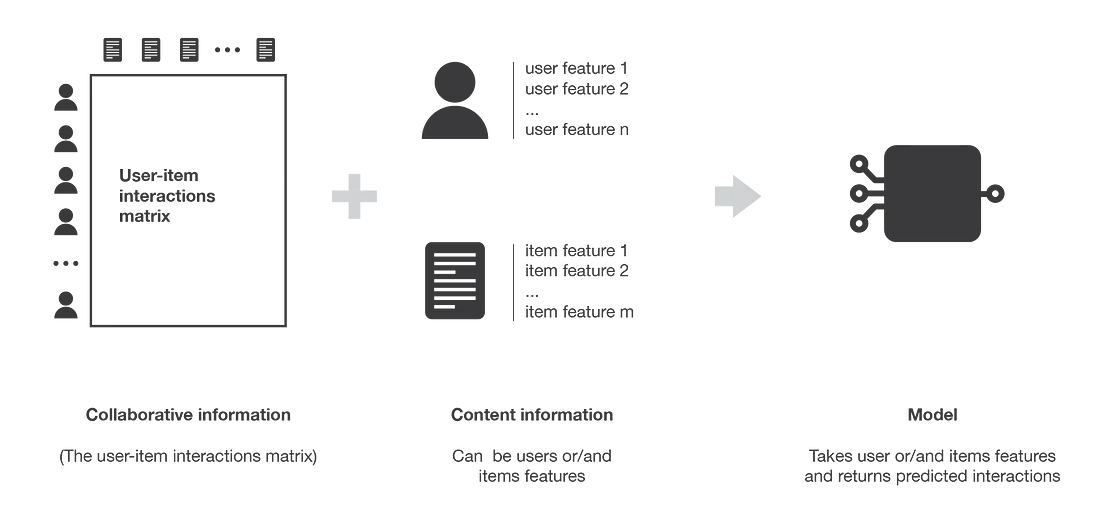
\includegraphics{images/Internet_05.jpg}
\end{marginfigure}

简而言之,推荐系统就是一种使用数据分析和机器学习技术向用户推荐他们可能感兴趣的相关信息(电影、视频、物品)的算法。推荐系统常用的算法主要包括协同过滤,聚类和深度学习等。其中协同过滤是打造个性化推荐时的常用算法,可以分析出与用户有相似兴趣的群体,从而推荐该群体感兴趣的商品给客户。而聚类算法是将未知对象进行归类的算法,在构建智能推荐系统时,若缺失此前用户数据,可选用聚类算法。深度学习算法则是使用深度神经网络分析用户数据来输出用户感兴趣的商品。

实际上,推荐系统并不只是在电商平台上才有应用。社交软件如微信,陌陌,可以根据用户的好友关系和互动记录,推荐给用户新的朋友和内容。视频平台,如哔哩哔哩,抖音等,可以根据用户观看和点赞过的视频来推荐更多相关的视频内容,每次拉下屏幕刷新都是平台的推荐系统计算分析出的用户最可能感兴趣的视频。还有音乐平台,如网易云音乐和QQ音乐,打开每日推荐或是私人漫游,便是推荐系统根据用户听过的歌的风格来给用户量身定制的音乐节目单。

推荐系统让我们每个人都能享受个性化的定制服务,这时也有人会提出担忧“人工智能是不是给每个人都打造了一个信息茧房,所有人会都被困在里面一辈子”。这一点是不可否认的,推荐系统在给每个人个性化的推荐的同时,也变相地限制了每个人能获得的信息,我们很难得到和我们平时所处圈子外的信息,因为推荐系统会认为那些信息都是用户不会感兴趣的,也就不会推送到用户面前。但实际上,相比于人工智能大火前,我们每个人能获取到信息的渠道都十分的有限,在那时候,我们又何尝不是处在一个信息茧房中呢?在人短短的一生中,或许我们能在此信息茧房中得到的信息已经远远超于没有互联网的时代。更进一步地说,信息爆炸的时代,或许是这些基于人工智能技术的推荐系统才让我们免于淹没在信息的海洋中,获得属于我们自己个人的舒适圈吧。

\section[智慧客服]{智慧客服:AI为用户答疑解惑}

\begin{marginfigure}
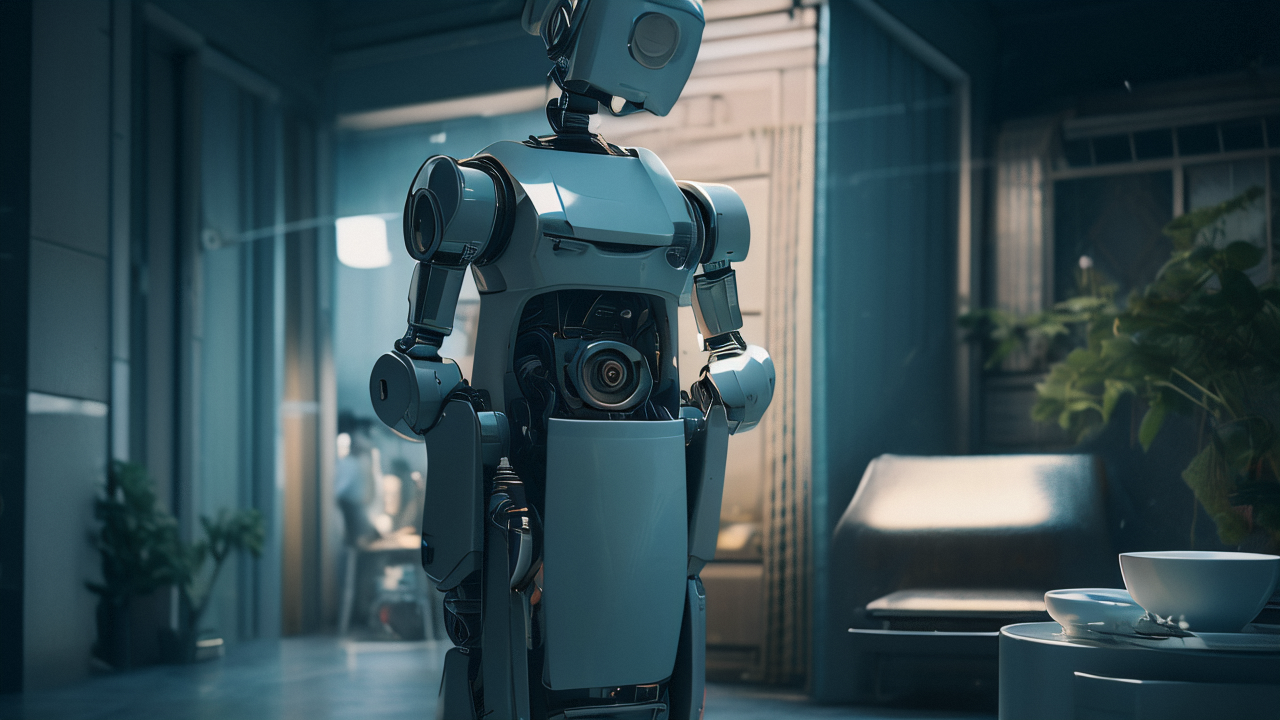
\includegraphics{images/Internet_07.png}
\end{marginfigure}

有一天,你突然接到一个电话,对面自称是某公司的客服,向你调查产品使用体验。如果你配合客服的请求,继续跟他对话,你一点也不会怀疑他是不是真人,因为他能很从容地和你进行交谈,逻辑也毫无漏洞。但是如果你突发奇想,问他一句“你是真人吗”,他或许就会立即宕机,陷入沉默。现在的智慧客服已经不再像过去只能让用户按0或1回答,而是能轻松处理语音文本,并且生成文本,转换为语音来进行对话,然而对于一些刁难的问题,智慧客服却仍然不能很好地处理。那么这样的人工智能的智慧客服是如何进行流畅的对答,又是为何无法回答一些问题的呢?

使用人工智能技术的智慧客服的原理实际上和手机中自带的语音助手类似,它们的整个工作流程都可以分为三步:自动语音识别(ASR),自然语言理解(NLU),语音合成(TTS)。

\section[智能家居与物联网]{智能家居与物联网:AI让生活更智能}

\begin{marginfigure}
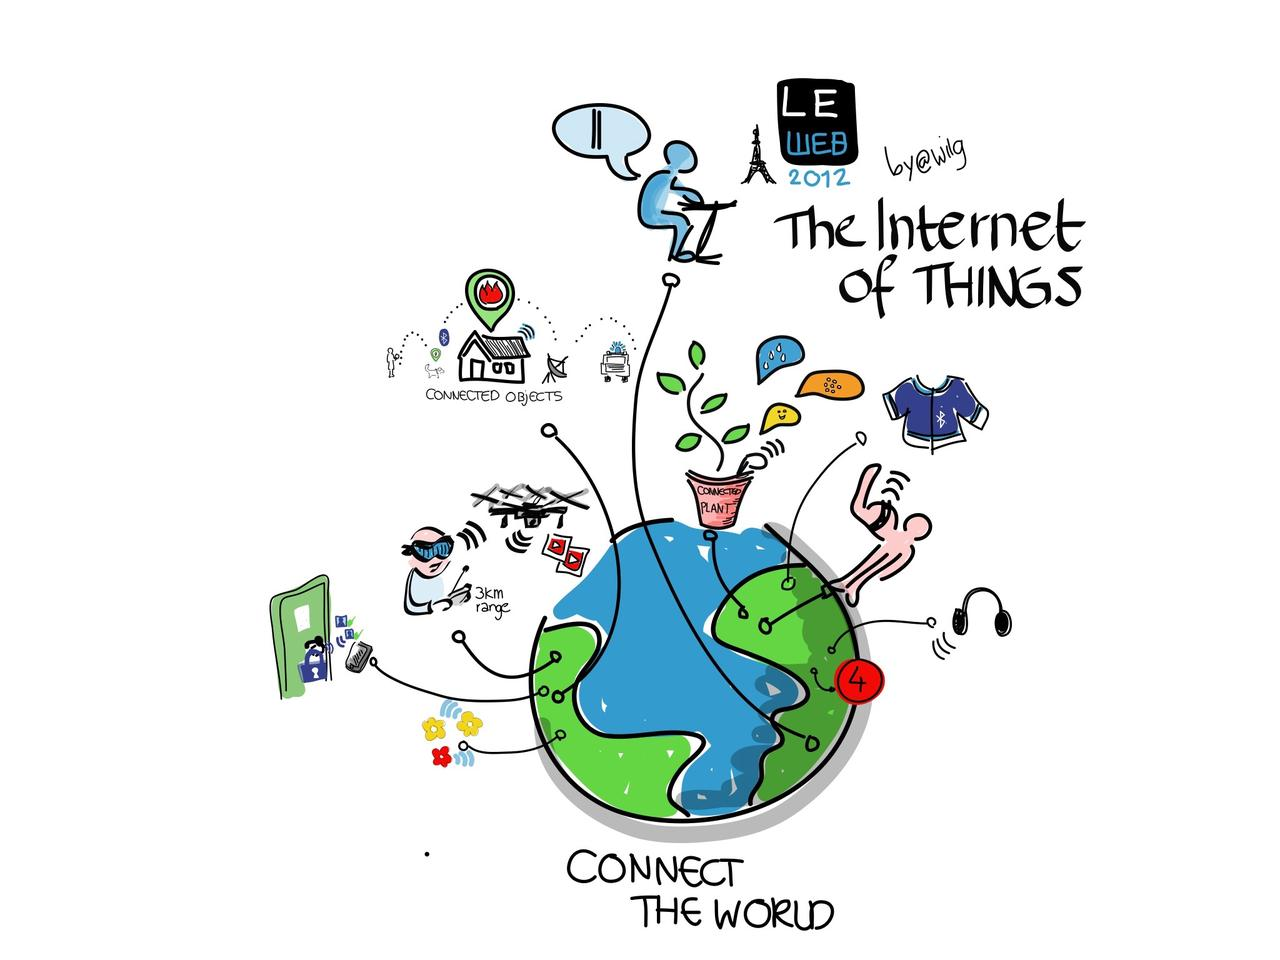
\includegraphics{images/Internet_08.jpg}
\end{marginfigure}

一个炎热的夏天,你工作了一天,拖着疲惫的身体在回家的路上,尽管已经是夜晚了,但白天的余热仿佛仍从地面不断传出来。你打开手机,发现手机上出现了一个提示,询问是否需要开启家中的空调。你毫不犹豫的点击了“是”。一踏入家中,清凉的空调风吹出来,你马上感觉浑身清爽了许多,与此同时,家中的灯也自动打开了,音响也在播放着你最近在音乐软件上收藏的音乐,家里的冷清感立马少了许多。一切都是那么的智能,仿佛有一个专属于你的仆人在家中等着你回家。如此智能的生活便是得益于当前智能家居的广泛使用了。在这小节,我们将探讨AI技术是如何让生活更加的智能和便捷的。

智能家居是指通过先进的信息技术、通信技术和自动化控制技术,将家庭内的各种设备、设施和系统互联互通,实现家庭管理、设备控制、能源管理、安全监控等功能,提高生活品质和便捷性的系统。其原理基于物联网、人工智能、传感器技术等多种技术的综合应用。这些技术的综合应用,使得家庭内的各种设备能够相互配合,实现更加智能化和自动化的控制,从而让我们的生活更加便捷和舒适。

智能家居系统主要可以包含以下几个部分:
1. 家庭网络:为智能家居设备提供网络连接和数据传输通道。
2. 智能设备:如智能照明,智能安防,智能家电等,负责数据采集,处理和执行。
3. 控制中心:作为智能家居系统的核心,负责设备控制,数据分析和决策制定。
4. 用户界面:为用户提供直观,便捷的操作界面,如手机APP,触控面板。
        智能家居的整体工作流程可以总结为:1. 传感器等物理设备收集家中的现实物理信息,并上传到物联网上。2. 物联网整合所有的传感器信息,通过控制中心进行数据分析和决策制定。3. 最终在手机APP上呈现给用户,让用户选择操作。

\subsection{物联网技术在智能家居中的应用}
智能家居的根本就是家居之间的联动,而联动的基础很大程度上依赖于物联网。为了了解智能家居的原理,我们需要首先熟悉物联网。物联网(Internet of Things,简称IoT)是一种将各种物理设备,传感器,软件通过网络连接起来的技术。通过网络连接起来的设备能够进行交互和通信,从而实现数据的采集,传输和分析,以此实现智能化的管理和控制。物联网的核心技术包括传感器技术、通信技术、数据处理技术、云计算和大数据等。通过这些技术,物联网可以实现对各种设备和物品的远程监控、管理和控制,使它们具有感知、认知和自主决策的能力。

通过物联网技术,可以完成绝大部分用户日常生活所需的“智能”。如智能照明中,物联网技术可以实现对家庭照明的远程控制和自动调节。用户可以通过手机APP或语音助手调节灯光的亮度、色温和开关状态。同时,智能照明系统还可以根据用户的作息时间和环境光线自动调整灯光,实现节能和舒适度的优化。除了简单的照明系统外,物联网还为家庭安防提供了多种方案。例如用户可以通过手机实时查看家中的摄像头画面,随时了解家庭安全状况。此外,智能门锁、门窗传感器和人体红外传感器等设备可以帮助用户实时掌握家庭出入情况和异常状况。

小米公司推出的大部分家居产品都可以通过米家软件进行连接,通过该软件,用户可以在手机上控制所有的家居的开关,也可以轻松获得家居的状态信息。更进一步的,其推出的手机回家模式和睡觉时开启晚安模式让用户的生活变得更加便捷,当手机连接到家中的wifi时,家中灯光自动打开,电动窗帘会自动拉上,空调自动打开,为了安防而设置的摄像头也自动关闭。而在用户的手机在晚间充电时,智能系统就会默认用户需要睡觉了,家中灯光自动关闭,窗帘会自动拉下来,手机也会调整至睡眠模式,避免用户在睡眠时被打扰。如此智能的系统,仅需要物联网就能实现。在人工智能技术火起来后,人们自然会想到如何应用人工智能技术来插入到智能家居系统中,从而让智能家居更加的“智能”。

\subsection{AI在智能家居中的应用}
通过物联网整合的数据可以传输给机器学习模型,模型可以从中学习到用户的生活习惯,从而优化家居设别的运行,以此来提供更为个性化的服务。下面将探讨AI在智能家居里的两个经典应用场景。

\begin{marginfigure}
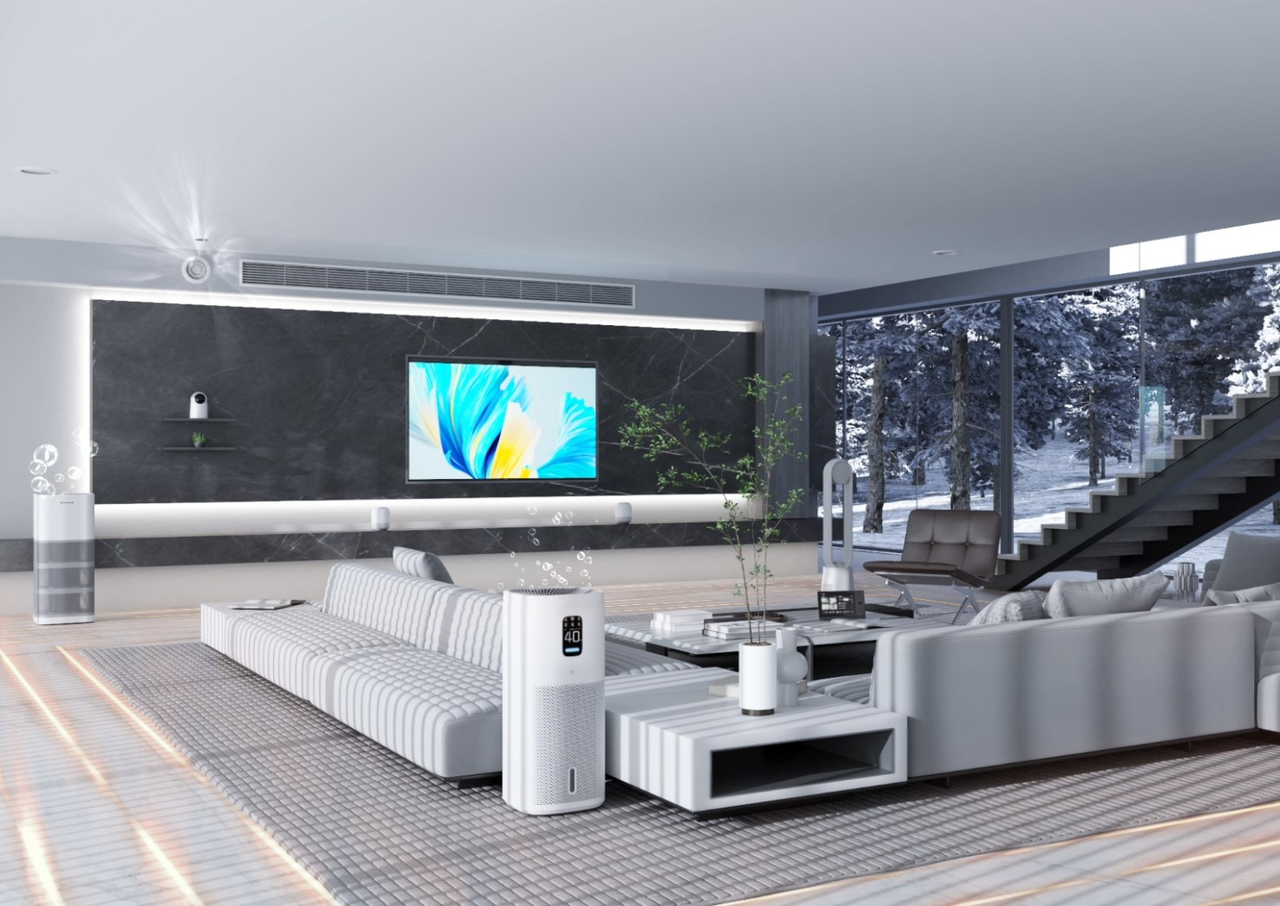
\includegraphics{images/Internet_09.png}
\end{marginfigure}

或许你的家中放置的电器越来越多,但是每个月的电费却仍然没有多大的变化,实际上这便是人工智能在你不知道的角落为你节省了一大笔电费了。通过物联网技术,智能家居系统可以实时收集家庭用电数据,包括用电量、用电时间、用电设备等信息。然后,利用AI算法对这些数据进行分析和处理,挖掘出用户的用电习惯和规律,这样模型就可以识别出用户在特定时间段内经常使用的电器设备,以及这些设备的用电量和用电时间。基于用户的用电习惯,AI算法可以对家庭用电进行智能调度和优化。例如,当用户不在家时,AI算法可以自动关闭不必要的电器设备,以减少能源消耗。同时,AI算法还可以根据用电高峰和低谷时段,智能地调整家电的运行时间,避免在高峰时段使用高耗能设备,降低家庭用电成本。此外,AI算法还可以根据天气、季节等因素,预测家庭的能源需求,并据此进行用电调度。例如,在冬季,AI算法可以预测室内温度需求,提前开启空调等取暖设备,避免能源浪费。而在夏季,AI算法可以预测室内制冷需求,合理调度空调、风扇等设备,实现舒适的室内环境,同时降低用电成本。

除了智能的用电调度外,智能家居还可以通过收集家庭成员的健康数据,例如体重、心率、睡眠质量等。同时,系统还可以获取家庭成员的生活习惯信息,如饮食、运动、作息等。基于这些数据,智能家居系统利用AI算法进行分析和处理,为每个家庭成员提供个性化的健康建议。例如,当系统检测到某个家庭成员的体重增长过快时,可以推荐合适的运动方案和饮食建议,帮助其控制体重。对于有慢性病的家庭成员,智能家居系统可以收集其相关生理指标,如血糖、血压等,并与医生远程协作,为患者提供个性化的治疗建议和康复计划。此外,智能家居系统还可以根据每个家庭成员的年龄、健康状况和生活习惯,为其提供定制化的生活提醒。例如,对于年长的家庭成员,系统可以提醒其按时服药、注意饮食健康;对于年轻的家庭成员,系统可以推荐科学的运动方案和健康的生活方式。

\subsection{智能家居面临的挑战}
尽管当前智能家居已经越来越普及,人们的生活也因此变得更加便捷和舒适,但智能家居仍面临着一些挑战需要解决。智能家居面临的一个重要的问题就是其安全性问题,因为智能家居产品涉及个人隐私和财产安全,而熟练的黑客则可以访问智能家居的互联网设备。在2016年10月,一个名为Mirai的僵尸网络渗透了DVR,摄像机和路由器的互联设备,通过拒绝服务攻击(也称为DDoS攻击)摧毁了主要网站的主机。此外,不同设备之间的互联也将是一个智能家居将要面临的问题,未来的智能家居将会涉及到不同类型和品牌的智能设备的互联。为实现智能家居的互联互通,可能还需要制定通用的智能家居设备协议和通信标准,以便不同品牌和类型的设备之间进行互联。

\section[AIGC]{AIGC(AI Generated Content):AI如何成为内容创作者}
这两年来,除了能够流畅地和人交流的ChatGPT外,AI领域最出圈的就是AI作曲和AI绘画了。在过去人们总是认为人工智能只能做一些无聊重复的工作,最不可能被代替的就是人们引以为傲的艺术相关的工作了。然而SunoAI和OpenArt等工具的出现直接颠覆了人们的想象,它们让人类不再能以傲慢的眼光看待AI。

\subsection{AI写诗}
月明清影里,露冷绿樽前。
赖有佳人意,依然似故年。--九歌
早在2017年,在央视的黄金档节目《机智过人》上,人们就发现人工智能已经可以写出媲美人类的诗歌了。在节目上,清华矣晓沅团队开发的作诗机器人「九歌」就展现出了惊人的创作能力,写出的诗歌先后淘汰了北大和武大的学生,成功闯进决赛。直到决赛前,大多数人都还以为九歌创作出的诗歌是人写出来的。这说明人工智能创作的诗歌已经能成功混淆视听,媲美人类创作的作品了。开头的这一段诗句就是人工智能创作出来的,不得不说,无论是诗句的连贯度,还是词句中流露的情感,都已与真人创作的无太多异处,相信大部分的人都无法分辨出这首诗的作者是人还是AI了。那么如此"智能"的AI创作者的原理究竟是什么呢,它又是如何被"创作"出来的?

AI写诗是人工智能中的自然语言处理的经典生成任务,不管是传统的机器学习方法,如隐马尔可夫模型,贝叶斯模型,还是当前广为使用的神经网络模型,如循环神经网络,Transformer,都可以轻松完成写诗的任务。

以循环神经网络为例,输入一些字词(如用户希望的诗歌的开头),模型可以一步一步预测下一个字,预测出的下一个字会和前面所有输入的字一起作为下一个时刻的输入,然后模型可以继续预测下一个时刻的字,以《静夜思》为例:当用户输入"床"字,模型会先基于"床"预测出"前"字,预测出的"床"作为下一个时刻的输入,模型会基于"床前"输出"明"字,如此反复,一共预测4次,即可输出完整的"床前明月光"
- 时刻1: 输入:"床",输出"前"
- 时刻2: 输入:"前",输出"明"
- 时刻3: 输入:"明",输出"月"
- 时刻4: 输入:"月",输出"光"

然而循环神经网络容易出现"遗忘"的问题,举个例子,在上面的时刻4的时候,模型很容易忘记较前时刻的输入"床"和"前",在输入"月"的时候,模型有很大可能只记得"明"字,基于"明月"输出的可能就是"夜"了。针对该问题,Transformer模型被提出来了。Transformer模型通过引入自注意力(self-attention)机制和多头注意力(multi-head attention)机制来捕获输入序列中的长依赖关系。不仅如此,不同于循环神经网络的串行的预测方式,Transformer能够并行进行预测,即输入"床"字,模型可以直接输出"前明月光",如此一来生成诗歌的效率也大幅度的提升了。

基于神经网络的写诗模型通常需要大量的诗歌数据进行学习训练才能输出符合人类审美的诗歌。尽管诗歌的好坏很大程度上都是主观的判断,但我们仍然可以通过设计一些客观的评价函数来评价模型输出的诗歌的质量,如诗句的连贯性,主题的相关性等。通过不断优化这些指标,模型就可以从诗歌数据中学习到词句的连接。

\begin{marginfigure}
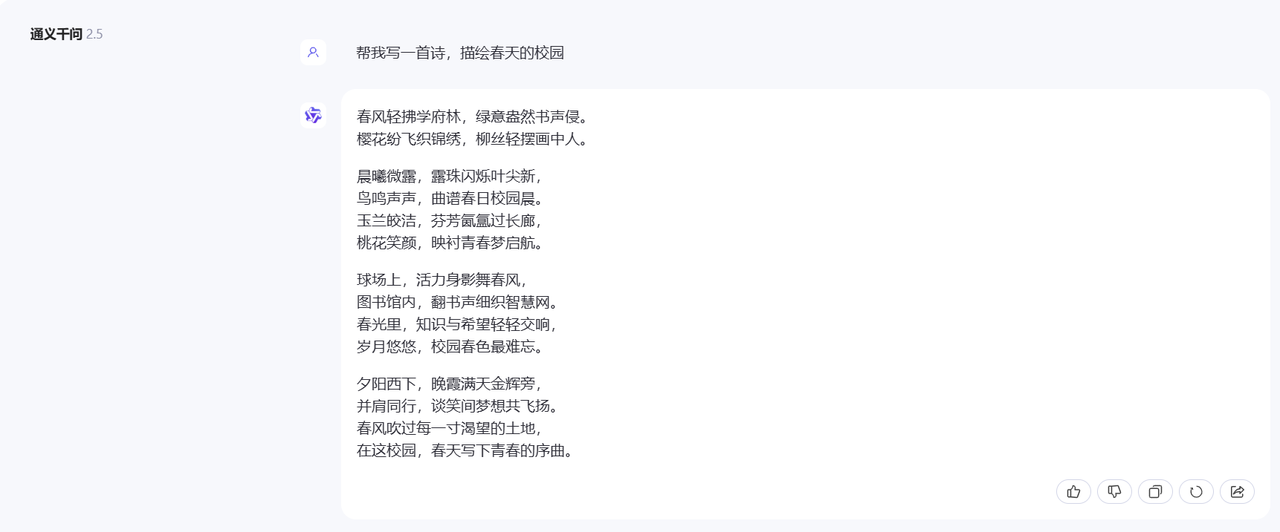
\includegraphics{images/Internet_10.png}
\end{marginfigure}

\subsection{AI绘画}
\begin{marginfigure}
    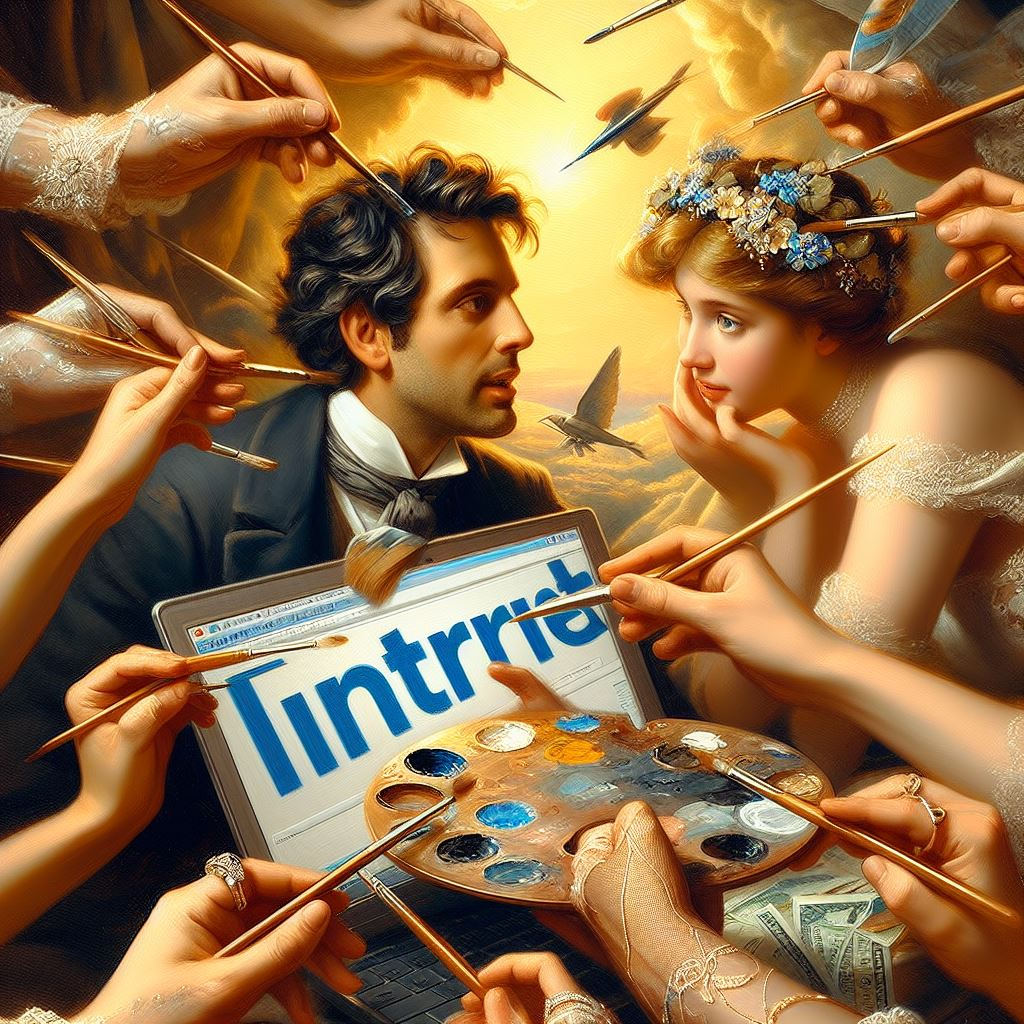
\includegraphics{images/Internet_01.jpg}
\end{marginfigure}
曾经画家为了创作一幅画需要不断构思,不断修改,花费多少个日日夜夜才能得到一个满意的作品,然而如今人们只需要下达几个简单的文字指令,AI就能自动画出多张精致的作品。而在众多的AI绘画模型中,Stable diffusion无疑是现今使用的最为广泛,最广为认知的了。

Stable diffusion是一款由Stablility AI公司于2022年所开发的AI绘画生成模型。由于该模型操作简便,且生成速度快,平均只需要10到20秒即可获得一张精致的画作,一经推出就受到广大网友的喜爱。那么这款模型具体是怎么运作的呢?

具体地说,Stable diffusion用的是latent diffusion model(隐扩散模型)。这是一种文本到图像的深度学习模型,输入文本,模型即可输出相关的图像。它一共由三个模块组成,分别是(变分自动编码器)VAE,文本编码器和U-Net。输入文字描述,该模型通常可以分为下面几步运作:
1. 首先模型随机生成图像,变分自动编码器把该图像从像素空间压缩到更小维度的隐空间。
2. 对隐空间中的图片添加噪声,进行扩散过程。
3. 通过文本编码器将输入的描述语转换为去噪过程的条件。
4. 基于文本编码器得到的条件,U-Net会对图像进行去噪。
5. 最终使用变分自动编码器将图像从隐空间转换回像素空间,得到图像。
除了输入文字描述得到相应图像,通过把中间的文本编码器替换成图像+文本的编码器,模型还可以完成基于文字描述对输入图像进行修改的功能。

\subsection{AI作曲}
实际上,在SunoAI出现前,就有几款AI作曲的工具出现了,如网易天音,SongR等。不得不承认的是,这些较早期的AI作曲工具都是有作曲能力的,但相对于强人工智能,这些产品都只能算得上是“工具”的范畴,使用这些工具需要使用者具有一定的音乐的理论知识。然而作为一款针对音乐人的工具,它们的生成逻辑又显得过于机械化,没有给人们太多的自由度去创作。因此这些工具也就逐渐淡出了人们的视野。

SunoAI,作为音乐界的ChatGPT,在2024年的3月推出,一经推出便轰动了世界。和以前的AI作曲不一样,SunoAI只需要用户输入一句话的提示词,既可以在短短数秒内生成一首几分钟的完整的歌曲,从作词,作曲,到人声演唱一气呵成,大大降低了普通人创作音乐的门槛。已经习惯了各类“AI歌手翻唱”的听众和用户迅速拥抱了Suno,从《宫保鸡丁咏叹调》到《让我们荡起双桨》重金属,从英语、日语、俄语到普通话甚至是粤语,网友们自发上传的作品包罗万象,网易云音乐、QQ音乐等平台也迅速上线了SunoAI音乐专区,甚至还推出了定期更新的官方推荐歌单。

\section[网络安全与隐私保护]{网络安全与隐私保护:AI如何护航互联网安全}
当前的网络空间已经进入到了人工智能时代。人工智能对网络空间已经产生了深远的影响,是人工智能时代的安全问题呈现出了新的趋势。一是攻击者开始运用人工智能发起新型网络攻击;二是出现了针对人工系统本身的攻击或欺骗,从而导致人工智能模型出现一些分类或预测的错误;三是人工智能开始赋能安全,也即人工智能保障安全,是指利用人工智能来自动识别潜在的网络威胁的工具和技术。在这一章节,我们将讨论当前人工智能如何护航互联网安全。

\subsection{恶意代码智能分析检测}
近年来,网络空间面临严峻的安全威胁,其中,僵尸网络,木马,蠕虫攻击就是威胁的典型代表。恶意代码作为攻击的载体,会在互联网上进行传播,可以定向传输至被攻击的目标。被攻击目标若运行了这些恶意代码,会造成信息泄漏,数据损失,主机失陷等后果。在2017年,一种名为WannaCry的病毒在全球范围内引起了一阵风暴,这种病毒正式利用Windows系统的SMB服务相关漏洞进行传播,所有被病毒缠上的主机上的图片,文档,音频,视频,压缩包,可执行程序等文件会被加密,如果这些受害者不支付赎金,被加密的文件将会无法恢复。

恶意代码分析中引入机器学习方法的一般工作模块可以分为:数据预处理模块,特征工程模块,机器学习训练模块。根据不同的恶意代码的类型,会采取不同的预处理方法,然后再选择人工定义和自动提取相结合的特征工程方法,通过特征工程模块输出的特征向量作为机器学习训练模块的输入,进行有监督的学习,最后训练好的分类器可以应用于实际的恶意代码检测。

以PE二进制恶意代码为例,给出一个具体的技术方案。首先,在数据预处理模块中,将待检测的PE二进制格式可执行代码在虚拟机中运行,监控并记录所产生的系统API调用序列;然后,对获得API序列进行特征工程,其中可以用N-gram模型,word2vec模型等方法将API序列转换为特征向量,这样就完成了机器学习前的工作。将特征向量作为机器学习模型的输入,机器学习模型则可以有很多选择,具体模型性能需要结合具体的场景来分析,可以使用传统的机器学习分类器如决策树,支持向量机,XGBoost等,亦可以使用神经网络模型,如卷积神经网络等深度学习分类器。通过在大规模的有监督数据上进行学习,模型可以获得较好的检测恶意代码的能力。

\subsection{恶意网页识别}
由360安全中心发布的《2019年网络诈骗趋势研究报告》显示,2014到2019年,网络诈骗人均损失逐年增长。当前的诈骗网站已经不局限于通过钓鱼网站来盗取用户的隐私数据,虚拟信贷,网络赌博等新型诈骗网站层出不穷。随着互联网的飞速发展,诈骗网站的内容也在不断变化,行为越来越难以检测,发展态势日趋产业化。

针对恶意网页日益增长的趋势,当前很多浏览器如Google Chrome,Edge等都已经可以检测识别出恶意网页,在用户点击网站时,若浏览器检测出其恶意攻击行为,就会阻止用户进入网站,从而保护了用户的个人隐私和财产安全。而这样的技术基本都是基于人工智能技术的,下面我们以中国移动提出的一个基于人工智能的诈骗网站识别方案为例,具体说明人工智能是如何为互联网安全保驾护航的。

诈骗网站识别方案的整体流程可以分为以下5个部分:
1. 收集活跃域名
2. 域名发现与拓展
3. 域名取证分析
4. 人工审核
5. 域名封堵
首先,从互联网数据中获取活跃的域名,利用人工智能模型来检测分析出潜在的诈骗域名,然后通过爬虫软件对潜在诈骗域名进行内容的爬取和分析,筛选出高度疑似诈骗网站的网站,交由人工进行审核,最后对于可以确定的诈骗域名进行封堵操作。这套恶意诈骗网站识别方案在2019年上线应用,每天会分析超过200亿条上网日志,垃圾短彩信,用户举报,每月能检测出诈骗网站超4万个,组断了2004.9亿次的诈骗网站访问,有效地保护了用户的个人隐私和财产安全。

第一步的域名发现会对网络中存在访问行为的域名进行搜集,并将这些域名信息作为全网的活跃域名全集。活跃域名全集的数据来源包括垃圾短彩信中的域名信息,用户投诉举报数据中的域名信息,以及用户的上网日志等。进而通过消息智能分类,域名智能分类,注册备案分析,流量日志分析,从收集得到的活跃域名全集发现潜在的诈骗域名。
域名拓展
活跃域名全集中的域名发现模块能够识别出可能的诈骗网站,但这意味着域名识别的时机已经晚于用户的访问,形成了事后识别的情况。然而,通过引入域名拓展模块,可以有效地填补域名发现模块的缺陷,甚至在现实网络中用户访问行为被监测到之前,就能发现并识别出潜在的诈骗网站,从而实现对诈骗网站的事前管理。
域名拓展模块具有根据已知欺诈域名信息进行进一步挖掘和发现的功能,可以找到更多与已知欺诈域名有关联的潜在欺诈域名,它由网站外链拓展、备案信息拓展、域名数字拓展和相似风格拓展四个子模块构成。
网站外链拓展:一些欺诈网站,如赌博类和色情类网站,通常会通过友情链接或广告的方式互相链接,方便用户在网站之间进行跳转。网站外链拓展模块利用这一特点,对已知欺诈网站中的外链信息进行迭代爬取,重点抓取欺诈网站中的友情链接和广告链接,以发现更多的潜在欺诈域名。
注册信息拓展:欺诈网站的创建者通常会批量注册大量的域名,我们可以利用域名注册信息的属性关联性来实现域名的拓展。注册信息拓展模块通过已知欺诈域名的备案联系人信息,反查该联系人注册的其他域名信息,将这些域名作为潜在欺诈域名。
域名数字拓展:在赌博类欺诈网站的域名中,通常会包含大量的数字。域名数字拓展模块对已知欺诈域名中的数字进行尝试性改变,以拓展域名,然后通过爬虫爬取并验证可访问性,从而获取潜在的欺诈域名。
相似风格拓展:欺诈网站的创建者在选择域名时,往往会倾向于特定的域名风格。相似风格拓展模块利用人工智能技术,学习已知欺诈域名的组成风格,然后利用人工智能的创作能力,生成更多与已知欺诈域名风格相似的潜在欺诈域名。由于人工智能技术生成的域名可能并不真实存在,因此需要结合爬虫技术,排除掉无法访问的潜在欺诈域名。
域名取证分析
内容分析取证模块对潜在诈骗域名的网站内容进行全面评估,从而找出高度疑似的诈骗网站,并将相关爬取内容作为判断依据提交给人工审核。在爬取网站的过程中,需要收集网站的文本信息、源码信息、图片信息,同时需要对网站的最终展示效果进行截图。收集到网站内容信息后,内容分析取证模块从文本、源码、图片、视觉等多个角度对网站进行诈骗特征分析,并将高度疑似的诈骗网站提交至人工审核平台。
人工审核
尽管当前的人工智能检测恶意诈骗网站的准确率已经很高,但是仍然会出现部分识别错误的情况,如把没有攻击行为的网站识别为恶意诈骗网站。因此我们还需要人工审核来确定网站是否为诈骗网站。对于恶意诈骗网站,人工审核平台会向域名封堵模块下达封堵指令
域名封堵
为了能够有效防止用户访问诈骗网址,域名封堵模块将判定为诈骗域名加入拦截名单,当有用户请求 拦截名单中的域名时,则中断用户请求,并向用户请求重定向到安全提示页面。
% \setchapterstyle{kao}
\setchapterpreamble[u]{\margintoc}
\chapter{车轮下的智慧}

随着人工智能技术的快速发展,交通与物流行业正经历一场前所未有的变革。AI的应用不仅极大地提升了效率,降低了成本,还在改变我们的出行方式和城市交通系统的构建。在本章的开头,我们将探讨人工智能如何引领交通与物流行业的未来发展,特别是在共享出行、智能交通网络、无人机物流、自动驾驶、应急响应等方面的创新应用。

共享出行的革命
共享出行是AI技术改变城市交通的一个突出示例。通过算法优化,共享出行平台能够实时分析交通数据,预测需求并优化车辆分配。这不仅提高了出行效率,还有助于减少交通拥堵和环境污染。例如,通过集成深度学习模型,共享汽车和电动自行车可以根据用户的出行历史和实时交通情况,提供个性化的路线建议和车辆推荐。

智能交通网络
在智能交通系统中,AI技术的应用更是体现了其对大规模运营的重大影响。城市可以利用AI来监控和管理交通流,实现信号灯的自动调整,减少交通延误和事故发生率。此外,AI也使得交通预测更为准确,帮助城市规划者在高峰时段合理调配资源,优化整个城市的交通布局。

无人机物流的兴起
随着无人机技术的成熟和规模化应用,物流行业也迎来了翻天覆地的变化。AI驱动的无人机能够在复杂的环境中自主导航,实现快速、精确的货物配送。这种新型的物流方式不仅提升了配送效率,还能到达传统物流难以覆盖的偏远地区。例如,AI系统可以分析天气数据和地形信息,自动规划出最佳的飞行路线,确保货物安全、及时地送达目的地。

自动驾驶技术的应用
自动驾驶汽车是AI在交通领域应用的重头戏。随着机器学习算法和传感技术的不断进步,自动驾驶汽车能够实现更为精准的环境感知、决策制定和操作执行。这些车辆能在各种天气和交通条件下安全行驶,显著减少交通事故,提升道路使用效率。例如,谷歌的Waymo自动驾驶车辆已在多个城市进行测试,展示了其在城市和郊区环境中的行驶能力。此外,自动驾驶车辆在长途货运中的应用也正在逐步展开,预计将大幅降低物流成本并提高行业的安全标准。

智能仓储与物流优化
物流行业中的AI应用不限于运输。在仓储管理上,AI能够优化库存管理,预测产品需求,自动调整存货水平。通过机器人自动化技术,仓库的拣选和包装过程也已实现高度自动化,大幅提升操作效率。例如,亚马逊的仓库就广泛采用了机器人和AI系统来优化其物流流程,这不仅加快了处理速度,还提高了整体的物流效率。

城市交通的智能化管理
AI的另一个重要应用是在城市交通管理系统中的智能化。通过安装传感器和摄像头,结合AI分析,城市管理者能够实时监控交通状况,及时响应交通拥堵和事故。这种系统可以优化交通流动,比如通过动态调整交通灯周期,优化公交车和地铁的运行时间表。例如,北京市已经实施了基于AI的交通管理系统,该系统能有效预测和缓解交通高峰时段的压力。

AI在应急响应中的作用
在交通事故或极端天气条件下,AI也能发挥关键作用。通过实时数据分析,AI可以快速定位事故发生地,自动调度救援资源,并优化救援路径。此外,AI还能分析历史数据预测潜在的高风险区域,提前部署必要的安全措施,从而减少事故的发生。

随着AI技术的进一步发展,我们可以预见到更多革命性的变革将会出现在交通和物流行业。自动驾驶汽车将在未来的城市交通系统中扮演越来越重要的角色,而AI在车联网中的应用将使得交通管理更加智能化、高效化。此外,随着大数据和云计算技术的支持,AI将能够实现更深层次的交通优化,为城市交通带来更多的可能性。在本章中,我们将深入探讨这些技术的具体应用案例和它们将如何塑造未来的交通与物流行业。通过具体的分析和展望,我们可以更好地理解人工智能技术在推动社会进步方面的重要作用和潜力。

\section{自动驾驶技术:AI如何赋能汽车自主行驶}
自动驾驶技术是近年来人工智能领域的一大突破,它的发展不仅预示着交通方式的根本变革,还代表着对安全、效率和环境影响的显著改进。自动驾驶汽车(Autonomous Vehicles, AVs)通过集成先进的人工智能技术,能够实现无人驾驶。在本节中,我们将深入探讨自动驾驶汽车的关键技术原理,包括传感器融合、计算机视觉与对象识别,决策制定与路径规划、控制系统与执行动作,以及解析AI如何在这些过程中起到核心作用。
\subsection{传感器融合与环境感知} 
自动驾驶汽车的环境感知能力是其安全操作的基石。在这一领域中,传感器融合技术起着至关重要的作用。传感器融合是一种利用多种传感器数据的技术,通过这些数据的整合处理,提高自动驾驶系统对环境的感知精度和可靠性。自动驾驶车辆通常配备有雷达、激光雷达(LIDAR)、摄像头和超声波传感器等设备,每种传感器都有其独特的优势和局限。

雷达技术 主要用于探测对象的距离和速度。雷达波可以在各种天气条件下穿透雾和雨,提供远距离的物体检测能力,这对于高速行驶的自动驾驶汽车至关重要。例如,高速公路上的自动驾驶汽车需要从远处探测到前方车辆的速度和位置,以便及时调整行驶状态。

激光雷达 则通过发射数百万个激光点并测量它们反射回来的时间,来创建周围环境的详细三维地图。激光雷达提供的高分辨率数据使得自动驾驶汽车能够精确地识别车道边界、行人、非机动车及其他障碍物。尽管激光雷达在雨雪天气中的性能会受到一定影响,但其在晴朗天气条件下的表现无疑是精确和可靠的。

摄像头 是自动驾驶系统中不可或缺的组成部分,它负责捕捉视觉信息,如道路标志、交通灯和道路线条。现代自动驾驶车辆上的高分辨率摄像头能够在不同的光照条件下进行有效工作,通过先进的图像识别算法,摄像头能够识别各种交通标志和信号,为自动驾驶提供必要的规则遵循指导。

超声波传感器 主要用于低速行驶和停车过程中的近距离检测。它们能够探测到车辆周围的小障碍物,如在停车时的路边石或其他车辆,是实现精确停车和低速操控的关键技术。

传感器融合不仅仅是物理层面上多传感器的简单叠加,更重要的是在数据处理和解析层面,通过算法将来自不同源的数据综合考虑,形成一个统一的、全面的环境感知结果。在实际操作中,这通常通过一系列复杂的数据融合算法完成,如卡尔曼滤波器和粒子滤波器,这些算法能够有效地整合来自不同传感器的信息,弥补各自的不足,提高整体的感知能力和准确性。

AI在传感器融合中扮演着至关重要的角色。通过深度学习和机器学习技术,AI能够对从传感器收集到的大量数据进行实时分析和处理。例如,利用卷积神经网络(CNN)处理来自摄像头的图像数据,可以实现对交通标志和行人的高精度识别;同时,结合来自雷达和激光雷达的空间位置信息,AI系统能够更准确地判断对象的距离和速度,预测其可能的移动路径。

总而言之,传感器融合技术和AI的结合,不仅极大地增强了自动驾驶汽车的环境感知能力,也为实现真正的自动驾驶奠定了坚实的基础。随着技术的不断进步和成熟,未来自动驾驶汽车将能够在更加复杂和多变的道路环境中安全高效地行驶,彻底改变我们的出行方式。

\subsection{计算机视觉与对象识别}
计算机视觉在自动驾驶汽车中扮演着至关重要的角色,它使车辆能够“看”到并理解其周围的世界。这一技术领域涉及图像捕捉、处理及分析,使车辆能够识别和解释道路上的各种对象,如行人、其他车辆、交通标志和信号等。在自动驾驶技术中,计算机视觉不仅是实现安全驾驶的基础,更是确保车辆能够准确响应环境变化的关键。

视觉数据的获取与处理
自动驾驶车辆通常装配有多个摄像头,这些摄像头位于车辆的前部、后部、侧面等不同位置,以捕获360度的视觉信息。这些高分辨率的摄像头能够在不同光照和天气条件下捕获清晰的图像,为后续的图像处理和分析提供原始数据。
图像数据获取后,接下来的步骤是通过高级图像处理技术对这些数据进行预处理,包括图像去噪、对比度增强和颜色校正等,以提高图像质量并准备进行更深层次的分析。
特征检测与对象识别
在预处理之后,计算机视觉系统利用深度学习模型,尤其是卷积神经网络(CNN),来识别和分类图像中的对象。这些模型通过大量的训练数据学习识别各种交通标志、行人、车辆以及其他重要的道路元素。
例如,自动驾驶系统中的一个标准操作是使用目标检测算法,如YOLO(You Only Look Once)或SSD(Single Shot MultiBox Detector),这些算法能够在图像中快速精确地定位和识别不同的对象。这些算法的优势在于它们可以实时地在视频流中识别对象,这对于动态的驾驶环境至关重要。
语义分割与场景理解
除了简单的对象识别外,更复杂的计算机视觉任务如语义分割,它将图像中的每个像素分类到一个特定的类别,这对于完全理解道路场景非常重要。语义分割技术可以帮助自动驾驶车辆区分道路、人行道、车道标记等,从而在复杂的交通环境中作出更精确的驾驶决策。
深度感知与立体视觉
为了更好地理解三维空间中的对象和环境,自动驾驶汽车还会利用立体视觉技术。立体视觉通过比较从两个或多个摄像头获得的图像差异,来计算对象的距离。这一技术与传统的单摄像头视觉系统相比,可以提供更多的深度信息,对于判断车辆与其他对象的相对位置和速度非常有用。
面向未来的发展
随着AI和计算机视觉技术的不断进步,未来自动驾驶汽车的视觉系统将更加强大和智能。研究人员正在开发更先进的算法,以提高在极端天气条件下的表现,如在雨、雾或雪中有效操作。此外,增强现实(AR)和虚拟现实(VR)技术的融合可能会为驾驶提供更丰富的视觉信息和辅助,进一步提高安全性和驾驶体验。
通过这些先进技术的应用,计算机视觉不仅增强了自动驾驶汽车的环境感知能力,也为实现全自动驾驶的未来奠定了坚实的基础。这些技术的进步意味着自动驾驶汽车将能够在更广泛的条件和环境下安全高效地运行,最终实现无人驾驶的承诺,为我们的道路交通带来革命性的变革。
\subsection{决策制定与路径规划}

自动驾驶汽车的核心能力之一是在复杂的道路环境中做出准确的决策并规划合适的行驶路径。这一过程涉及到高级算法和机器学习技术的应用,确保车辆能够在保证安全的同时,有效地从一个地点移动到另一个地点。

理解决策制定的框架
决策制定在自动驾驶技术中通常分为几个层次:策略决策、行为决策和运动规划。策略决策层面涉及到目的地的选择和高层次的路线规划,如何从当前位置到达目的地的整体策略;行为决策则是在行驶中需要做出的选择,例如何时变道、超车或停车;最后,运动规划则是具体到车辆如何在瞬间调整其速度和方向以执行这些决策。

路径规划与算法
路径规划是决策制定过程中的重要环节,它确保汽车能够在遵守交通规则的同时,选择最优的行驶路径。常见的路径规划算法包括A*算法、Dijkstra算法和Rapidly-exploring Random Tree (RRT)算法等。这些算法能够帮助自动驾驶系统评估各种行驶路径的可行性、安全性和效率,选择最合适的一条。

例如,A*算法通过评估从起点到终点的最佳路径,并考虑实际行驶中可能遇到的各种因素,如道路条件、交通状况和环境障碍等,来动态规划路径。这种算法不仅计算最短距离,还能优化行驶时间和能耗。

行为决策与机器学习
在行为决策方面,自动驾驶车辆需要能够实时做出反应,如何在复杂交通中安全地变道、应对突然出现的障碍物或其他紧急情况。这需要车辆具备高度的环境感知能力和快速的决策能力。利用机器学习,尤其是强化学习,自动驾驶系统可以通过不断的试错和训练,学习在特定情况下采取最合适的行动。

强化学习在自动驾驶汽车的决策制定中扮演着重要角色,它允许车辆在模拟环境中“经历”各种复杂的交通场景,从而学习如何在现实世界中做出最优决策。通过这种方式,车辆能够学习从人类驾驶员的行为中提取的最佳实践,同时也能自行发现独特的策略来应对前所未见的情况。

整合决策与执行
一旦决策被制定和路径被规划,下一步就是执行。这需要车辆的控制系统精确地调整车辆的速度、方向和其他操作。自动驾驶汽车的控制系统使用一系列的算法,如PID控制器和模型预测控制(MPC),来确保决策得以精确实施。

PID控制器通过调整车辆的实际状态与目标状态之间的差异来工作,适用于简单的调节任务。而模型预测控制则更为复杂,它不仅考虑当前的误差,还预测未来的动态变化,并进行优化计算,以期达到最佳的控制效果。这使得自动驾驶汽车能在保证安全的同时,实现更加平滑和自然的驾驶体验。

通过这些先进的技术和算法,自动驾驶汽车在进行决策制定与路径规划时能够展现出类似人类的适应性和灵活性。这些能力的持续提升将使自动驾驶汽车在未来的道路上运行得更加安全、有效和智能。

\subsection{控制系统与执行动作} 
控制系统是自动驾驶汽车技术中的核心组成部分,它负责将高层次的决策转化为具体的驾驶动作,如加速、转向和制动。这一过程中,高度精确和可靠的执行至关重要,因为它直接影响到行车的安全性和舒适性。控制系统的设计和优化是确保自动驾驶汽车能够在复杂多变的道路环境中稳定运行的关键。
控制系统的基本框架
自动驾驶汽车的控制系统通常包括几个基本组成部分:输入设备、控制算法和执行机构。输入设备负责收集车辆的实时状态信息,如速度、位置和周围环境的数据。控制算法则根据这些信息以及从决策制定模块接收到的指令,计算出相应的控制信号。最后,执行机构根据这些信号调整车辆的具体行为,包括转向角度、油门开度和刹车力度等。
控制算法的作用
在自动驾驶系统中,控制算法是实现精确驾驶动作的核心。这些算法必须能够在极短的时间内做出响应,以适应快速变化的道路条件。常用的控制算法包括:
•	比例-积分-微分 (PID) 控制器:PID控制器是一种经典的控制算法,它通过调整控制量来减少目标值与当前值之间的偏差。在自动驾驶汽车中,PID控制器可以用于调节车速和保持车道等基本任务。
•	模型预测控制 (MPC):MPC是一种更高级的控制策略,它利用预测模型来预测未来一段时间内的车辆状态,并优化当前的控制动作。MPC特别适用于处理动态复杂的驾驶情境,如紧急避障和复杂的车辆交互情况。
•	学习控制器:随着机器学习技术的发展,越来越多的自动驾驶系统开始采用基于学习的控制策略,如强化学习。这类控制器可以通过大量的模拟和实际驾驶数据学习如何在特定情境下做出最优的控制决策。
执行机构的重要性
执行机构是控制系统的“执行手臂”,它包括电动机、液压或气动系统等,负责物理地实现转向、加速和制动等动作。在自动驾驶汽车中,执行机构的设计和性能直接影响到控制命令的准确性和响应速度。
•	电动助力转向系统(EPS):EPS通过电动机提供转向助力,它允许更精确的控制转向角度,适应不同的驾驶条件。
•	电子刹车系统:这种系统通过电子信号控制刹车,而非传统的机械链接,提高了刹车的响应速度和可靠性。
•	电动节气门控制:在现代汽车中,节气门的开闭由电子控制,这使得油门响应更加精确,有助于实现更平滑的加速过程。
面临的挑战与未来方向
尽管现有的控制系统已经能够支持许多高级的驾驶辅助功能,但自动驾驶技术仍面临诸多挑战,尤其是在极端天气条件或复杂交通环境中的表现。未来的研究将继续集中在提高控制算法的鲁棒性和适应性上,例如通过集成更多类型的传感器数据和采用更复杂的机器学习模型来进一步优化控制策略。
此外,随着车辆通信技术(V2X)的发展,未来的自动驾驶汽车将能够不仅仅依赖于本车的传感器和控制系统,而是通过与其他车辆及道路基础设施的通信,实现更为协调和高效的控制执行,从而大大提高整个交通系统的安全性和效率。
\section{决策与规划:AI如何提升交通系统性能} 
在现代交通系统中,人工智能技术的应用已经成为提升效率、安全性和可持续性的关键因素。通过利用各种数据来源,AI能够实时解析复杂的交通状况,优化路径规划,预测驾驶行为,并进行综合风险评估。这些能力不仅减少了交通拥堵,还有助于降低能源消耗和减少排放,从而推动了交通系统的整体性能向更高水平的发展。在实际应用中,智能出行服务如滴滴出行和各种地图应用程序已经集成了这些AI技术,提供了更加智能化、个性化的出行解决方案。下面,我们将深入探讨这一主题的两个重要方面。
6.2.1 AI驱动的路径优化与交通管理

在现代城市的交通管理中,AI的应用已经成为推动效率提升和拥堵减少的重要技术。通过智能算法的支持,交通系统能够更加灵活地适应城市的动态变化,优化交通流,减少环境影响,并提升用户出行体验。以下详细探讨AI如何驱动路径优化和交通管理。
实时数据分析与动态路径规划
AI系统的核心在于其能力进行快速、高效的数据分析和决策。通过集成来自GPS设备、交通摄像头、车载传感器以及用户输入的实时数据,AI可以构建一个全面的交通流动图。利用这些数据,AI算法不仅可以为单个用户提供最优路径规划,还能预测整个城市的交通流变化,从而优化交通信号调度和路线建议。
例如,地图应用程序如Google Maps和高德地图等,利用复杂的算法来分析用户的旅行时间和路线偏好,同时考虑实时的交通状况,如事故、道路封闭或高峰时段的交通拥堵。这些应用程序能够动态调整推荐的路线,以避开拥堵区域,减少旅行时间和能源消耗。
智能交通信号与流量管理
除了为单个车辆提供路线建议,AI也在城市级别的交通管理中发挥着越来越重要的作用。通过安装智能交通信号灯,结合AI分析技术,城市管理者可以实时调整交通信号的时长和序列,以适应交通流量的实际变化。这种类型的系统可以显著减少等待时间,优化交通流通效率,降低交通拥堵。
在一些先进的实施案例中,如北京市的智能交通系统,AI技术被用来分析各主要交通路口的流量数据,智能调整信号灯的工作模式,甚至在特定情况下实现信号灯的主动绿灯波。这种系统的实施不仅改善了交通状况,还减少了车辆的怠速时间,进一步减少了空气污染和能源消耗。
路线优化与车队管理
对于商业运输和物流公司而言,AI同样能够提供显著的帮助。通过使用专门的车队管理软件,结合AI路径规划工具,公司可以优化其车辆的配送路线,确保货物以最经济的方式送达。这种优化不仅基于路线的长度和预计时间,还考虑了货物的特性、车辆的载重能力、以及司机的工作时间等因素。
例如,滴滴出行等共享汽车服务利用AI算法实时分配车辆,以满足用户需求的同时最大化司机的工作效率。这种优化算法考虑了多种因素,包括车辆位置、目的地、交通状况以及预测的需求模式,从而使得车辆分配更加合理,减少空驶里程,降低能耗和排放。
6.2.2 高级行为预测和风险管理
在现代交通系统中,AI的应用不仅限于路径规划和交通流优化,还扩展到了行为预测和风险管理的领域。通过对大量数据的分析和模式识别,AI能够预测驾驶者的行为,评估潜在的风险,并采取措施以预防事故,从而大幅提升道路安全性和效率。
行为预测技术的应用
行为预测是AI在交通管理中的一个重要应用,它涉及对驾驶者行为的预测,包括他们的驾驶习惯、反应时间以及在特定情况下的可能行为。通过收集和分析来自车辆传感器、摄像头和历史数据的信息,AI可以识别模式并预测驾驶者在未来某一时刻的行为,例如变道、减速或停车。这种预测能力对于提高交通系统的响应速度和减少事故具有重要意义。例如,在高速公路上,AI系统可以通过分析车速和车辆间距来预测可能发生的碰撞,并提前警告驾驶者或自动调整车速,从而避免事故的发生。
风险评估的实现
风险评估是另一个关键应用,AI通过实时分析环境数据和驾驶行为来评估潜在的安全风险。这包括对道路条件、天气情况、交通密度以及驾驶者的注意力和疲劳程度的综合评估。通过这些信息,AI可以识别高风险情景并采取措施来缓解这些风险,比如调整交通信号灯的时序,提醒驾驶者注意潜在的危险,或在极端情况下,采取自动驾驶措施控制车辆。
在实际应用中,地图应用程序和导航系统通过集成天气和交通数据,能够向驾驶者提供关于最安全路线的建议。例如,如果某条路线因为恶劣天气或事故而变得危险,AI系统可以推荐一个替代路线,从而避开潜在风险。
与滴滴等平台的整合
在共享出行平台如滴滴出行中,AI的行为预测和风险管理技术尤为重要。这些平台利用AI分析驾驶者的行为模式和评价系统,以确保乘客的安全。AI系统可以评估驾驶者的驾驶质量,包括他们的行车速度、制动习惯和总体驾驶风格,从而识别出潜在的高风险驾驶者并采取必要的措施,如提供培训或限制其接单。
此外,通过分析历史事故数据和驾驶行为,AI可以帮助平台优化其调度系统,使驾驶者在行驶过程中避开高风险区域,例如在夜间或恶劣天气条件下减少对事故高发区的派单。

\section{物流:AI智能调度} 
在现代物流和快递行业中,人工智能的应用已成为提升效率和响应速度的关键技术。特别是在处理庞大的订单量和复杂的配送需求时,AI智能调度系统能够有效地优化资源配置,减少送货时间,并提高整体服务质量。顺丰、菜鸟等快递巨头已经开始利用AI技术来革新传统的物流模式,通过智能算法来优化配送路线、管理仓库、预测需求,并自动调配最适合的运输方式。这一章节将深入探讨AI如何在物流行业中实现智能调度,从而提升运营效率和顾客满意度。
6.3.1 优化配送路线与车队管理
在快递和物流行业中,配送路线的优化和车队管理是提升效率和降低运营成本的关键。通过人工智能技术,公司能够实现这些目标,从而提供更快、更可靠的服务。以下详细探讨AI在优化配送路线和车队管理方面的应用。
AI在配送路线优化中的作用
配送路线优化是物流管理中的一个复杂问题,涉及到多个变量和约束,如交通条件、配送时间窗、车辆载重限制和驾驶员工作时间等。AI通过使用高级算法如遗传算法、模拟退火或蚁群优化算法来解决这些问题,为每个配送任务生成最优路线。
这些算法模拟自然选择过程中的“适者生存”原则,通过迭代过程逐步优化路线配置。例如,遗传算法通过模拟DNA交叉和突变来优化路线选择,能够在复杂的约束条件下找到近似最优解。这种方法不仅考虑了最短行驶距离,还考虑了如何最大限度地减少交通拥堵和其他潜在的延误,从而节省时间和燃料。
利用实时数据进行动态调度
随着物联网(IoT)技术的发展,物流车辆装备了各种传感器,实时传输位置和状态数据。AI系统可以利用这些数据进行实时动态调度,根据当前交通状况、天气条件和车辆状态自动调整配送路线和计划。
例如,如果某条主要道路因事故而中断,AI系统可以即刻重新计算所有受影响车辆的路线,指导它们绕行,以避免延误。此外,如果某一配送任务突然取消或新增,系统也可以立即重新优化整个车队的配送计划,确保资源得到最有效利用。
车队管理的智能化
除了路线优化,AI还在车队管理方面发挥着重要作用。通过分析历史数据和实时信息,AI可以帮助物流公司做出关于车队规模、车辆购买与租赁、维护计划以及驾驶员排班的决策。
智能车队管理系统能够监控每辆车的性能和维护需求,预测可能的故障,并在问题发生前安排维修,减少意外故障造成的服务中断。此外,系统还可以根据驾驶员的工作时间规定和个人表现,自动安排驾驶员的班次,确保合规同时也最大化工作效率。
与顺丰、菜鸟等快递行业的集成
在实际应用中,顺丰、菜鸟等快递行业巨头已经在利用AI技术来优化他们的物流服务。顺丰利用自家的算法优化配送路线,提高配送速度和准确性,同时减少了运营成本。菜鸟网络则通过其智能物流平台,实现了包裹跟踪、仓储管理和配送优化,提升了客户满意度和操作效率。
这些公司的成功案例表明,AI技术的应用能够显著提升物流行业的服务质量和经济效益。未来,随着AI技术的进一步发展和应用扩展,物流行业的智能调度和管理将更加高效和智能化,能够更好地应对市场需求和挑战。
6.3.2 智能仓库管理与需求预测
在现代物流系统中,仓库管理和需求预测是确保供应链效率和响应速度的关键环节。通过人工智能技术的整合,物流公司可以实现仓库操作的自动化、优化存货管理,以及通过精确的需求预测来提前做好准备,从而显著提升整体运营效率。
AI在智能仓库管理中的应用
仓库管理的自动化和智能化是AI在物流行业中应用的显著特点之一。通过使用机器人、自动化货架系统和高级的管理软件,智能仓库可以提高货物处理的速度和准确性,减少人力需求和操作错误。
1.	自动化货物搬运:在许多现代仓库中,自动化机器人被用于拣选、搬运和排序货物。这些机器人能够在仓库内自由移动,通过扫描货物上的条形码来验证和更新库存信息,同时将货物从存储区域运送到打包站或装载区。
2.	智能货架系统:智能货架系统可以实时监控库存水平,自动识别缺货或过剩情况,并向管理系统发送更新。这种系统通过减少手动检查库存的需要,提高了仓库管理的效率。
3.	高级视觉系统:利用计算机视觉技术,智能仓库可以对进出货物进行视觉检查,自动识别损坏或错误商品,确保出库的质量控制。
需求预测的精准化
需求预测是物流和供应链管理中的一个复杂问题,涉及到对未来市场需求的准确预测,以便合理规划库存和生产。AI通过分析历史销售数据、市场趋势、季节性变化、促销活动以及其他外部因素,能够提供比传统方法更为准确的需求预测。
1.	时间序列分析:AI模型可以使用时间序列分析来预测未来的需求波动。这种方法考虑了数据中的季节性模式和趋势,能够预测出未来某段时间内的需求高峰或低谷。
2.	机器学习模型:更复杂的机器学习模型,如随机森林和神经网络,可以从大量的历史数据中学习,识别影响需求的关键因素。这些模型能够处理更多的变量和更复杂的数据关系,提供更精准的预测结果。
结合顺丰和菜鸟网络的实践
在实际应用中,顺丰和菜鸟网络等领先的物流公司已经在使用AI来优化仓库管理和需求预测。例如,菜鸟网络通过其智能物流平台,不仅自动化了仓库的多个操作流程,还能根据即时的销售和物流数据动态调整库存和配送计划。顺丰利用AI进行需求预测,确保在不同地区根据预测的订单量调整仓库库存,减少运输成本并提高客户满意度。



% \setchapterstyle{kao}
\setchapterpreamble[u]{\margintoc}
\chapter{AI医学的奇迹}
\section{引言}
提及人工智能,许多人脑海中浮现的可能是科幻电影中的智能机器人或未来城市的智能生活。但实际上,AI技术早已悄然渗透到我们生活的各个领域,特别是医疗行业。AI的应用正以前所未有的速度改变着传统的医疗模式,为我们带来了“AI医学的奇迹”。

一、医学影像分析:医生的得力助手
在医学影像分析领域,AI技术的应用可谓是“神笔马良”般的存在。传统上,医生需要花费大量时间和精力去仔细阅读X光片、CT、MRI等复杂的医学影像资料,而AI技术的出现,使得这一过程变得更加高效和准确。

通过深度学习技术,AI可以自动识别和分析医学影像中的病变区域,帮助医生快速定位问题所在。不仅如此,AI还能对病变区域进行量化分析,为医生提供更准确的病情评估和治疗建议。例如,在肺癌筛查中的应用,AI能够自动识别肺部CT图像中的可疑结节,并给出结节的大小、形态、位置等详细信息,大大提高了肺癌的早期发现率。

二、个性化治疗:精准医疗的新时代
在个性化治疗方面,AI技术同样发挥着重要作用。通过对患者的基因信息、生活方式、医疗病史等大数据进行深度分析,AI可以预测患者可能面临的健康风险,并为医生提供个性化的治疗建议。

例如,在肿瘤治疗领域,AI技术可以根据患者的基因检测结果,预测肿瘤对某种药物的敏感性和耐药性,从而帮助医生为患者选择最合适的药物和剂量。这种基于AI的个性化治疗方案,不仅提高了治疗效果,还减少了不必要的药物副作用,让患者受益良多。

三、新药研发:加速药物创新的引擎
在新药研发领域,AI技术的应用更是如虎添翼。传统的新药研发过程往往需要耗费数年的时间和数亿美元的资金,而AI技术的引入,大大缩短了这一过程。

通过深度学习和大数据分析技术,AI可以对海量的生物数据和化学数据进行快速分析和筛选,找出具有潜力的药物候选物。同时,AI还可以预测药物在临床试验中的疗效和安全性,从而优化临床试验方案,提高试验效率。这种基于AI的新药研发模式,不仅加快了药物的上市速度,还降低了研发成本,为患者带来了更多福音。

四、医疗AI公司及产品:改变医疗行业的力量
在医疗AI领域,涌现出了许多优秀的企业和产品,它们正以前所未有的速度改变着医疗行业。
例如,迈瑞医疗推出的TE10/20系列超声搭载了心脏结构自动识别功能,大大提高了心脏超声检查的效率。开立医疗推出的凤眼S-Fetus则是全球首款基于动态图像对标准切面自动抓取的人工智能技术,为产前超声检查带来了颠覆性的技术体验。

此外,还有一些专注于人工智能辅助医疗影像诊断的公司,如医准智能等。它们通过深度学习技术,实现了对乳腺、肺部等多种疾病的智能辅助诊断,为医生提供了更加准确和高效的诊断工具。

五、AI医学的未来展望
随着技术的不断进步和应用场景的不断拓展,AI医学的未来充满了无限可能。

首先,AI技术将进一步提高医学影像分析的准确性和效率,为医生提供更加精准的诊断依据。其次,AI技术将在个性化治疗和精准医疗方面发挥更大作用,为患者提供更加个性化的治疗方案和健康管理建议。最后,AI技术还将加速新药研发的过程,为医疗行业带来更多的创新药物和治疗方法。

总之,AI医学的奇迹正在不断上演,它正在以前所未有的速度改变着医疗行业。我们有理由相信,在不久的将来,AI技术将为我们带来更多的健康福祉和生命奇迹。

\section{智能诊断:AI如何精确判断病情}
在医疗领域,疾病的诊断与治疗向来是医生们面临的重要挑战。随着科技的飞速发展,AI技术逐渐崭露头角,为医学诊断带来了革命性的变革。特别是在医学影像识别方面,AI以其独特的学习和分析能力,正在逐步改变医生们的工作方式和诊断精度。本文将详细介绍AI如何通过学习海量的医疗数据,辅助医生进行疾病的精确诊断和治疗,并聚焦于一些经典的AI工作,让读者对AI在医疗领域的应用有更深入的了解。
\subsection{AI辅助医学影像识别的崛起}
医学诊断中,医学影像识别一直是至关重要的环节。传统上,医学影像识别主要依赖于医生的专业知识和经验。然而,由于医生个人主观性和经验差异的存在,诊断结果往往存在一定的误差。幸运的是,随着AI技术的引入,这一局面正在发生深刻的变化。

AI辅助医学影像识别是基于深度学习技术实现的。深度学习是一种仿照人脑神经网络工作方式的机器学习方法。它通过构建多层次的神经网络模型,对大量的医学影像数据进行学习和训练,使得模型能够自动识别和提取图像中的关键特征。一旦模型训练完成,它就能够对新的医学影像进行快速、准确的识别和分析,为医生提供诊断的有力支持。

这种AI辅助医学影像识别的方法,不仅大大提高了诊断的准确性和效率,还弥补了医生个人经验差异可能带来的不确定性。通过AI的帮助,医生可以更加准确地识别和定位病变,从而更快地制定治疗方案,提高患者的治疗成功率。同时,AI还可以在繁忙的临床工作中为医生减轻负担,使其有更多时间去关注和照顾患者。

因此,可以说AI辅助医学影像识别的崛起不仅是医疗领域的一次革命性突破,也是对传统医学影像识别方式的一次重要补充和完善。随着技术的不断进步和应用的不断推广,相信AI在医学影像识别领域的作用会越来越大,为医学诊断带来更多的便利和精确性。
\subsection{深度学习在医学影像识别中的应用}
深度学习技术在医学影像识别中的应用非常广泛,涵盖了从基本的图像预处理到复杂的疾病诊断等多个方面。以下是一些经典的AI工作案例,它们展示了深度学习在医学影像识别中的强大能力。

1. CT和MRI图像分析
CT(计算机断层扫描)和MRI(磁共振成像)是两种常见的医学影像技术,它们能够提供高分辨率的医学影像数据。然而,这些图像中包含了丰富而复杂的信息,医生需要花费大量时间和精力进行解读和分析。深度学习技术通过对大量的CT和MRI图像进行训练和学习,能够自动识别和标记出病变区域,为医生提供快速而准确的诊断结果。
例如,一项名为“UNet”的深度学习模型在医学影像分割领域取得了显著成果。UNet模型采用了一种特殊的编码器-解码器结构,能够充分捕捉图像中的空间信息和上下文信息,从而实现对医学影像的精确分割。通过训练UNet模型,医生可以更加准确地定位病变区域,为治疗方案的制定提供有力支持。

2. X光图像分析
X光图像是另一种常见的医学影像技术,广泛应用于骨折、骨质疏松等疾病的诊断。然而,由于X光图像的灰度变化和噪声干扰等因素,医生在诊断过程中往往需要仔细观察和判断。而深度学习技术则可以通过对大量的X光图像进行训练和学习,自动识别和提取出图像中的关键特征,为医生提供辅助诊断的依据。
例如,一项名为“CheXNet”的深度学习模型在X光图像分析领域取得了突破性进展。CheXNet模型采用了卷积神经网络(CNN)技术,通过对大量的X光图像进行训练和学习,能够自动识别出图像中的多种疾病表现,如肺炎、肺结核、气胸等。通过CheXNet模型的辅助诊断,医生可以更加快速和准确地确定病情,为患者提供及时的治疗。

3. 眼科疾病诊断
眼科疾病诊断是另一个重要的应用领域。由于眼科疾病的种类繁多且症状复杂,医生在诊断过程中往往需要借助专业的设备和技能。而深度学习技术则可以通过对眼底图像和视网膜扫描图像进行学习和训练,自动识别和诊断出多种眼科疾病,如青光眼、黄斑变性等。
例如,一项名为“DeepEye”的深度学习模型在眼科疾病诊断领域取得了显著成果。DeepEye模型采用了卷积神经网络和循环神经网络(RNN)技术,能够自动从眼底图像中提取出关键特征,并结合患者的临床信息进行疾病诊断。通过DeepEye模型的辅助诊断,医生可以更加准确地判断病情,为患者提供更加个性化的治疗方案。

\subsection{AI辅助医学影像识别的未来展望}
随着技术的不断进步和应用场景的不断拓展,AI辅助医学影像识别的未来充满了无限可能。未来,AI技术将进一步提高医学影像识别的准确性和效率,为医生提供更加精准的诊断依据。同时,随着多模态医学影像数据的不断涌现和融合,AI技术还将实现对多种医学影像技术的综合分析和诊断,为医生提供更加全面和深入的病情评估。此外,AI技术还将与基因组学、蛋白质组学等其他领域的技术相结合,实现对疾病的全方位分析和预测,为医疗行业的未来发展开辟新的道路。

\section{药物研发:AI加速新药问世}
在医学的浩瀚宇宙中,药物研发一直是探寻未知、追求突破的重要领域。然而,传统的新药研发过程充满了艰辛与挑战,周期长、投入大、成功率低成为了困扰这一领域多年的难题。然而,随着人工智能(AI)技术的飞速发展,新药研发领域正迎来一场前所未有的变革。AI技术以其独特的学习和分析能力,正在逐步改变新药研发的面貌,为医药行业注入新的活力。

\subsection{AI与新药研发的相遇}
在传统的新药研发过程中,科学家们往往需要花费数年的时间进行大量的实验和研究,从成千上万的候选化合物中筛选出具有潜在疗效的分子,再通过复杂的临床试验验证其安全性和有效性。这个过程不仅需要投入巨大的人力、物力和财力,而且成功率极低。据统计,一款新药从研发到上市往往需要10年以上的时间,投入超过10亿美元的资金,而成功率却不足10%。

然而,AI技术的出现为新药研发带来了全新的可能性。通过深度学习和大数据分析技术,AI可以自动分析和处理海量的生物数据和化学数据,快速筛选出具有潜在疗效的候选化合物,大大缩短新药研发的周期和降低研发成本。同时,AI还可以预测药物在临床试验中的疗效和安全性,为药物研发提供重要的参考依据。

\subsection{AI辅助药物设计:从海量数据中筛选潜力分子}
在药物设计领域,AI技术的应用尤为突出。通过机器学习算法,AI可以自动学习和分析已知的药物结构和活性信息,建立复杂的预测模型。然后,这些模型可以被用来预测新的化合物是否具有潜在的疗效和安全性。这种方法被称为“基于机器学习的药物设计”。

具体来说,AI辅助药物设计可以分为以下几个步骤:
1. 数据收集与预处理:首先,AI需要收集大量的生物数据和化学数据,包括已知药物的结构、活性、作用机制等信息。然后,对这些数据进行预处理和清洗,确保数据的质量和准确性。
2. 特征提取与表示:接下来,AI需要从这些数据中提取出关键的特征信息,如化合物的分子结构、官能团、电荷分布等。这些特征信息将被用来表示化合物的“身份”和“特性”。
3. 建模与训练:在提取了特征信息后,AI需要构建复杂的预测模型。这些模型可以是神经网络、支持向量机、决策树等机器学习算法。然后,使用已知的药物数据对模型进行训练和优化,使其能够准确地预测新的化合物的疗效和安全性。
4. 候选化合物筛选:一旦模型训练完成,AI就可以开始筛选新的候选化合物了。通过输入新的化合物的特征信息到模型中,AI可以预测其是否具有潜在的疗效和安全性。然后,根据预测结果对候选化合物进行排序和筛选,选出最具有潜力的化合物进行后续的实验验证。

\subsection{AI辅助高通量药物筛选:快速找到有效药物}
除了辅助药物设计外,AI还可以在新药研发的高通量药物筛选阶段发挥重要作用。高通量药物筛选是一种通过自动化和并行化技术快速筛选大量候选化合物的方法。然而,由于候选化合物的数量庞大且结构复杂,传统的筛选方法往往效率低下且容易遗漏潜在的有效药物。

而AI技术可以通过对候选化合物的结构和活性进行深度学习和分析,快速预测其是否具有潜在的疗效和安全性。然后,根据预测结果对候选化合物进行排序和筛选,选出最具有潜力的化合物进行后续的实验验证。这种方法可以大大提高高通量药物筛选的效率和准确性,缩短新药研发的周期和降低研发成本。

\subsection{AI优化药物分子:强化学习、演化算法与深度生成模型的协同之旅}
在药物研发的后期阶段,对候选药物分子的优化和改进是至关重要的一环。这涉及到对药物分子结构的精细调整,以期望提高其疗效、降低副作用,并优化其生物利用度等特性。然而,由于药物分子设计的复杂性和多维度性,传统的方法往往难以在短时间内找到最佳解决方案。幸运的是,随着人工智能技术的飞速发展,我们有了更多强大的工具来应对这一挑战。

1. 强化学习:智能试错与反馈
强化学习是一种通过试错和反馈来进行学习的机器学习算法。在药物分子优化中,我们可以将强化学习框架应用于模拟的药物与靶点结合过程中。通过不断调整药物分子的结构,AI可以在模拟环境中尝试不同的分子构型,并根据与靶点的结合亲和力或其他相关指标来获得反馈。这种反馈将指导AI进行下一步的调整,直到找到具有最佳性能的药物分子结构。

2. 演化算法:模拟自然选择的智慧
演化算法是另一种强大的优化工具,它模拟了自然界中的生物演化过程。在药物分子优化中,我们可以将演化算法应用于生成和筛选候选药物分子。通过随机生成一系列初始的分子结构,并在每一代中根据与靶点的结合亲和力或其他性能指标进行选择、交叉和变异等操作,我们可以逐步演化出性能更优的药物分子。

3. 深度生成模型:创造与想象的边界
最近,深度生成模型在图像、文本和音频等领域取得了令人瞩目的成果。这类模型,如ChatGPT和DALL-E,能够通过学习大量数据来生成新的、高度逼真的内容。尽管分子是不同于视觉和自然语言的另一种全新数据模态,很多成熟的深度生成模型技术同样展现出了巨大的潜力。
深度生成模型可以学习已知药物分子的结构特征和性质,并生成新的、具有潜在疗效的分子结构。与传统的基于规则的生成方法相比,深度生成模型能够探索更广泛的化学空间,并生成更具多样性和创新性的候选药物分子。
此外,深度生成模型还可以与其他优化算法相结合,形成一个协同优化的框架。例如,我们可以先使用深度生成模型生成一批候选药物分子,然后利用强化学习或演化算法对这些分子进行进一步的优化和筛选。这种协同优化的方法能够充分发挥各种算法的优势,提高药物分子设计的效率和准确性。

4. 未来的展望
随着技术的不断进步和应用场景的不断拓展,AI在药物分子优化领域的应用将会越来越广泛。未来,我们可以期待更加智能、高效和精准的药物分子设计方法的出现。同时,随着多模态数据和跨学科技术的不断融合和发展,AI还将在药物研发的其他领域发挥更大的作用,为医药行业的创新和发展注入新的动力。

\subsubsection{AI在新药研发中的未来展望}
随着技术的不断进步和应用场景的不断拓展,AI在新药研发领域的应用将会越来越广泛。未来,AI技术将进一步提高新药研发的效率和准确性,为医药行业带来更多的创新药物和治疗方法。同时,随着多模态数据和跨学科技术的不断融合和发展,AI技术还将实现对药物研发全过程的智能化管理和优化控制,为新药研发提供全方位的支持和保障。

在这个充满机遇和挑战的新时代里,AI与新药研发的结合将会创造出更多的医学奇迹。让我们一起期待这场科技与医学的完美结合所带来的美好未来吧!

\section{健康辅助:AI健康管家}
随着科技的飞速发展,人工智能(AI)已经渗透到我们生活的方方面面,特别是在医疗健康领域,AI正以其独特的魅力和无限的可能性,成为我们的“健康管家”。从辅助残疾人士到智能检测设备,AI技术正在不断拓宽医疗健康服务的边界,让我们的生活更加便捷、健康。
\subsection{AI辅助残疾人士:温暖与智慧并行的关爱}

1. 深度学习技术:为视障群体点亮视界
在视障群体的生活中,视觉信息的缺失常常让他们面临诸多不便。然而,随着深度学习技术的不断进步,AI正在为这一群体带来前所未有的帮助。图像描述技术通过深度神经网络,将摄像头捕捉到的画面转化为详细的语音描述,让视障人士能够“听到”周围的世界。想象一下,一位盲人朋友只需携带一台装有AI图像描述技术的智能手机,就能“看到”街头的风景、超市的商品,甚至是亲人的脸庞,这无疑为他们的生活增添了许多色彩。

2. 语音+文本学习技术:打破沟通壁垒
除了视觉辅助外,AI还在语音和文本学习领域为视障人士提供了极大的便利。通过语音识别技术,AI可以将语音指令转化为文字信息,帮助他们更便捷地使用手机、电脑等电子设备。同时,AI文本转语音技术则能将电子文档、邮件等文字信息转化为语音输出,让视障人士能够轻松“阅读”各类资讯。这种双向的语音与文本转换技术,不仅极大地提高了视障人士的沟通效率,还让他们能够更深入地参与到社会生活中去。

3. 其他AI辅助技术:拓展生活的无限可能
除了上述技术外,AI还在其他方面为残疾人士提供了帮助。例如,通过深度学习技术,AI可以辅助肢体残疾人士进行康复训练,根据他们的身体状况和康复需求,提供个性化的训练计划和指导。此外,AI还能帮助听障人士进行语音识别和语音合成,让他们能够更流畅地与外界沟通。这些技术的出现,不仅为残疾人士带来了便利和关爱,还让他们感受到了科技的温暖和力量。

\subsection{AI检测设备:智能守护,健康无忧}
4. 智能手表:手腕上的健康管家
随着可穿戴设备的普及,智能手表已经成为许多人日常生活中不可或缺的一部分。这些小巧的设备不仅具备时间显示、信息提醒等基本功能,还集成了多种健康监测传感器,如心率监测、血氧检测等。通过AI算法对传感器数据的分析和处理,智能手表能够实时监测用户的健康状况,并在出现异常时及时发出提醒。例如,当用户的心率或血氧水平超出正常范围时,智能手表会立即发出警报,提醒用户及时采取措施。这种智能守护的方式,让人们在忙碌的生活中也能时刻关注自己的健康状况。

5. AI算法:精准分析,科学预测
在智能检测设备中,AI算法发挥着至关重要的作用。通过对大量用户数据的深度学习和分析,AI能够发现隐藏在数据中的规律和趋势,为用户的健康状况提供更为精准的分析和预测。例如,AI可以通过分析用户的心率、血压等数据,预测其心血管疾病的风险;通过分析用户的睡眠质量、运动量等数据,预测其心理健康状况。这些预测结果不仅能够帮助用户更好地了解自己的身体状况,还能为他们提供科学的健康建议和指导。

6. 远程医疗:打破地域限制,实现健康共享
随着5G、云计算等技术的发展,远程医疗已经成为现实。通过智能检测设备收集用户的健康数据,并借助AI算法进行分析和处理,医生可以远程为用户提供诊疗建议和治疗方案。这种远程医疗的方式不仅打破了地域限制,让更多人能够享受到优质的医疗资源,还提高了医疗服务的效率和便捷性。想象一下,一位偏远地区的患者只需佩戴一款智能手表或智能手环等检测设备,就能随时随地将自己的健康数据发送给远在城市里的医生进行诊断和治疗。这无疑为医疗健康领域带来了革命性的变革。

\section{结语}

AI在医疗健康领域的应用正逐渐展现出其巨大的潜力和价值。从辅助残疾人士到智能检测设备,AI正在以不同的方式改变着我们的生活和健康管理方式。未来,随着技术的不断进步和应用场景的不断拓展,我们有理由相信AI将为我们带来更多的惊喜和便利。让我们拭目以待这个充满智慧和关爱的时代吧!
% \setchapterstyle{kao}
\setchapterpreamble[u]{\margintoc}
\chapter{金融科技的升腾}
近年来,金融领域正在经历着数字化转型的浪潮,这一变革源于人工智能(AI)与各行业的紧密融合。传统金融机构从最初的基本能力探索逐渐发展为深度垂直整合,形成全面应用和持续创新的阶段。这个转型过程得益于金融机构庞大的客户群体、丰富可靠的数据资源以及强大的技术基础,使其成为高质量人工智能应用的理想场景。与此同时,人工智能技术的兴起,尤其是由ChatGPT等技术带来的狂潮,已经开启了新的应用发展时代。在政策引导、技术驱动和行业实践的共同作用下,人工智能技术在金融领域的广泛应用不断推动着金融供给侧结构性改革、增强金融服务实体经济的能力,同时有效地防范和化解金融风险。

在政策和业务需求双管齐下的背景下,人工智能在金融领域的应用呈现出前所未有的活力和潜力,人工智能在金融领域的应用成为一种趋势,改变着金融行业的生态,引领着金融业向数字化、智能化方向迈进。

在政策层面上,以“规范治理+科技与金融深度融合”为导向的扶持政策得到增强,主要由人民银行、银保监会、科技部等主体制定人工智能战略规划和相关政策。这些政策覆盖金融科技标准、数据安全与隐私保护、数据治理与应用、科技与金融场景深度融合等方向,以进一步促进人工智能与金融的融合,并深化人工智能在金融领域的应用。在业务层面上,人工智能与传统金融业务深度融合,为实体金融机构提供了强大的支持。各种人工智能技术,如机器学习、计算机视觉、知识图谱、自然语音处理、智能语音与对话式 AI,正在逐步在金融领域得以应用,解决了传统金融机构面临的运营成本高、供给不足、门槛高、信息不对称、风险评估难等问题。同样,人工智能在支付结算、存贷款与资本筹集、投资管理、市场设施等金融业务上的应用,帮助金融企业提高数字化能力,推动金融转型升级,开拓新的管理和商业模式,提升了服务实体经济的效率和能力。

人工智能技术在金融领域具有广阔的市场前景,近几年金融机构的技术投入增势显著,《金融科技(FinTech)发展规划(2022-2025年)》等相关政策为未来金融科技的重点投入及创新发展指明了方向,并驱动着金融行业数字化进程加速。艾瑞咨询数据显示,2022年中国银行业IT投入3068亿元,预计未来国内银行业IT投入规模仍将以约24.6\%的复合增长率保持高速增长态势,于2025年达到近6000亿元的规模投入。根据IDC数据显示,中国保险业总体IT投入从2018年的226.4亿元增长至2021年354.8亿元,2017-2021年复合增速为12.06\%。根据中国证券业协会数据统计,2017 年 -2020年,证券行业在信息技术领域投入由 159.86 亿元上涨至 262.87 亿元,2021年全行业投入338.2亿元,同比增长28.7\%。

这一系列数字清晰地表明,金融机构对人工智能技术的投入不断攀升,主要集中在夯实金融科技基础设施、前沿科技采购以及各个领域的技术资金投入。这种趋势不仅反映了金融机构对数字化转型的紧迫需求,同时也预示着人工智能在金融领域持续发展的巨大潜力。在这一过程中,金融机构将更加深度融合人工智能技术,推动金融市场进一步向智能化、数字化转型。


我国在AI+金融技术领域不断迭代创新,积极推动金融行业的数字化进程。在商业模式的解构中,我们可以将整个产业链划分为上游(基础层)、中游(技术层)和下游(应用层)三个关键层面。上游部分由综合技术、区块链、云计算、大数据等厂商主导,它们提供着金融行业数字化转型所需的基础设施支持。这些公司通过不断创新,为整个行业的数字化提供可靠的技术基石。中游则由各类技术公司主导,它们专注于提供人工智能算法、机器学习、生物特征识别、知识图谱等核心技术和解决方案。这一层面的公司在推动技术前沿的同时,也为下游应用层提供了关键的技术支持。在下游,这些先进技术得以广泛应用于金融业务领域,应用场景的多样性不断扩展。从智能营销、智能识别、智能投顾、智能风控到智能客服,这些应用不仅涵盖面广,而且深刻改变了金融服务的形态。金融机构通过引入这些先进技术,提升了运营效率、优化了风险管理,并拓展了服务范围,使得金融科技的融合更加贴近实际业务需求。

\section{信贷评估:AI重塑借贷关系}
\subsection{传统信贷评估的挑战}

在金融领域,信贷评估一直是至关重要的环节,它直接影响着金融机构与借款人之间的借贷关系。传统的信贷评估方法主要依赖于人工进行风险评估和信用调查,然而这种方法面临着一系列挑战。首先,信息不对称,即金融机构难以获取到借款人的全面信息,导致评估结果可能不准确。其次,评估标准的不一致性,不同金融机构的信贷评估标准存在差异,导致对借款人信用风险的评估结果不一致。此外,传统的信贷评估方法效率低下,因为需要大量的人力和时间,已经无法满足日益增长的信贷需求。最后,公平性问题也是一个重要的挑战,由于人为因素的介入,传统信贷评估可能存在主观偏见,导致借款人在获得融资时面临不公平的情况。

随着人工智能技术的迅猛发展,AI正逐渐成为重塑信贷评估方式的关键力量。传统的信贷评估方式往往依赖于人工进行风险评估和信用调查,存在着信息获取不足、评估标准不一、效率低下等问题。而AI技术的应用,通过大数据分析、机器学习和深度学习等手段,能够快速准确地评估借款人的信用风险,为金融机构提供更精准、高效的信贷决策支持。AI重塑了传统的借贷关系,不仅提高了风险控制能力,还为借款人提供了更便捷、公平的借贷服务。在数字化时代,AI信贷评估将成为金融行业不可或缺的一部分,为借贷关系注入更多科技创新的活力。
\subsection{人工智能在信贷评估中的应用}

人工智能技术的发展为改善信贷评估提供了新的解决方案。通过分析大数据和应用机器学习算法,人工智能可以更准确地评估借款人的信用风险,提高信贷市场的效率和公平性。

首先,通过利用大数据技术,人工智能可以收集和分析海量的借款人数据,包括个人信息、财务状况和信用历史。这种深度分析使得人工智能能够挖掘出隐藏在数据背后的规律和趋势,从而更准确地评估借款人的信用风险。其次,借助于训练机器学习模型,人工智能能够从历史数据中学习和识别不同借款人的信用特征,并预测借款人未来的信用表现。决策树、神经网络和支持向量机等机器学习算法的应用使得金融机构更好地理解借款人的信用状况,从而做出更准确的信贷决策。

智能风险评估是人工智能在信贷领域的又一重要应用。基于大数据分析和机器学习算法,人工智能可以实现智能化的风险评估。通过对借款人的个人信息、财务状况、信用历史等多方面数据的综合分析,人工智能可以生成准确的信用评分,帮助金融机构快速、准确地评估借款人的信用风险。这种智能化的风险评估方法不仅提高了评估的准确性,还提高了评估的效率,有助于金融机构更好地管理信贷风险。最后,人工智能不仅能够提供智能化的决策支持,帮助金融机构制定更合理的信贷政策和策略,还能为金融机构提供针对不同借款人的个性化信贷方案,促进信贷市场的健康发展,提高市场效率和公平性。这种智能化的决策支持有助于金融机构更好地满足借款人的需求,推动信贷市场的良性发展。

人工智能通过大数据分析和机器学习算法,为传统的信贷评估带来了革命性的变革。智能风险评估和智能决策支持等技术的应用,提高了信贷评估的准确性和效率,促进了信贷市场的发展和健康。然而,随着人工智能技术的不断发展,我们也需要加强对其潜在风险的监管和管理,确保人工智能在信贷领域的应用能够为社会经济的可持续发展做出积极贡献。

\subsection{应用案例:蚂蚁借呗}
蚂蚁集团是一家在金融科技领域拥有领先地位的公司,他们利用人工智能技术在信贷评估中取得了令人瞩目的成就。以其旗下的蚂蚁借呗(Ant Credit Pay)为例,这是一款基于大数据和机器学习算法的信贷产品。蚂蚁借呗通过分析用户在支付宝平台上的消费数据、交易记录、社交网络等海量数据,结合深度学习算法,对用户的信用风险进行智能评估。

首先,蚂蚁借呗通过大数据分析,收集和分析用户在支付宝平台上的各种数据,包括消费行为、还款记录、社交网络等。这些数据不仅包含用户的个人信息和财务状况,还包括了用户的消费习惯、社交关系等多方面信息。通过对这些数据的深度分析,蚂蚁借呗可以挖掘出隐藏在数据背后的规律和趋势,更准确地评估用户的信用风险。

其次,蚂蚁借呗应用了机器学习算法进行信用评估。通过训练机器学习模型,蚂蚁借呗可以从历史数据中学习和识别不同用户的信用特征,并预测用户未来的信用表现。借助于这些机器学习算法,蚂蚁借呗可以实现智能化的信用评分,帮助金融机构快速、准确地评估用户的信用风险。

通过大数据分析和机器学习算法的应用,蚂蚁借呗不仅提高了信贷评估的准确性,还提高了评估的效率。用户可以在支付宝平台上快速完成信贷申请,无需填写繁琐的申请表格和提供大量的证明材料。蚂蚁借呗还提供了个性化的信贷方案,根据用户的信用状况和需求,为用户提供最适合的借款方案。这种智能化的信贷评估方法为用户提供了更便捷、更高效的信贷服务,也为金融机构降低了风险,促进了信贷市场的发展。

蚂蚁借呗是蚂蚁集团在信贷评估领域的一项重要创新。通过大数据分析和机器学习算法的应用,蚂蚁借呗实现了智能化的信贷评估,为用户和金融机构提供了更高效、更便捷的信贷服务,促进了信贷市场的发展和健康。

\section{反欺诈与风控:AI守护金融安全}
\subsection{不可或缺的风险管理工具}
在当今数字化时代,金融行业面临着日益复杂和多样化的挑战,其中风险管理成为金融机构不容忽视的核心议题。金融机构面对着来自市场波动、经济变化、法律法规变化等多方面的风险挑战。有效的风险管理不仅能帮助金融机构及时识别、评估和应对这些风险,还能保护资产、维护声誉,并实现可持续的业务增长。通过制定适当的风险管理策略、建立健全的内部控制机制、采用先进的技术工具等措施,金融机构可以最大限度地降低风险带来的损失,确保业务的稳健发展。在当今竞争激烈、风险多变的市场环境中,高效的风险管理不仅是金融机构的责任,也是其长期成功的关键。

人工智能技术的应用正在成为金融机构应对这些挑战的重要策略之一。随着人工智能在反欺诈和风险管理中的应用越来越广泛,越来越多的金融机构正积极构建自己的“AI风控墙”。人工智能能够协助金融机构更加智能地识别和预防欺诈行为,提高风险管理的效率和准确性,从而保护客户的个人信息以及资金安全。通过智能化的数据分析和决策支持,金融机构能够更好地应对风险挑战,增强市场竞争力,促进行业的健康发展。

随着科技的不断进步,人工智能在金融领域的应用将不断扩展和深化。未来,金融机构将继续探索和应用更加先进的人工智能技术,进一步提升风险管理的水平和效能,为客户提供更安全、更可靠的金融服务,推动金融行业持续发展。

\subsection{智能风控:筑牢反欺诈防线}

在信息网络和数字化技术的不断普及的背景下,层出不穷的诈骗手段对人民的财产安全造成了严重威胁。由于人口基数大,对于诈骗犯罪的发现和管理难度也变得十分巨大,因此,人工智能在反欺诈和风险管理中发挥着越来越重要的作用,金融系统协助打击电信网络诈骗犯罪,践行“金融为民”理念刻不容缓。

人工智能可以通过分析大数据来识别潜在的欺诈模式和趋势,利用机器学习算法,系统可以从海量数据中提取特征,发现隐藏的模式,并预测可能的欺诈行为。其次,人工智能还可以实时监测交易和客户行为,识别异常模式和异常交易,从而及时发现并阻止可疑活动。此外,人工智能还能够自动化决策过程,根据预先设定的规则和模型对可疑交易进行风险评估,并采取相应的措施,如暂停交易或发出警报。通过智能化的数据分析和决策支持,有效提高了金融系统的安全性和稳定性,还为客户提供了更加可靠和高效的金融服务。

2022年开始,中信银行切实履行职责,通过技防和人防相结合,深层次筑牢金融反诈防火墙,切实保护金融消费者权益,有力保障了客户资金安全。其推出的“哨兵”智能风控系统可以利用大数据、机器学习和人工智能等先进技术,对银行交易和客户行为进行实时监测和分析,以识别和预防欺诈行为。这种做法不仅可以提高反欺诈的效率,还能降低银行和客户的风险,保护客户的资金安全和个人信息。

随着科技的发展,智能风控系统将不断优化和升级,为银行业提供更加可靠的安全防护。“哨兵”智能反欺诈系统通过在欺诈交易关键链路上引入公安、社交、电信等外部风险信息,利用机器学习和大数据技术,实现风控策略的动态调整,管控措施的梯度化和精准化,强化反诈预警能力与劝阻机制,及时发现潜在受害客户,并通过总分支三级联动响应机制,快速触达客户,第一时间协助客户摆脱诈骗人员的洗脑控制,及时阻止客户转账的行为,避免了客户的损失。

“哨兵”智能反欺诈系统包含三大核心科技助力全链条反诈。一是毫秒级异常交易精准识别。基于中信银行的强大算力,对每一笔交易进行事中侦测,毫秒级识别风险,实时触发差异化的安全机制和管控措施,主动拦截和劝阻被诈客户。二是AI模型精准防控。自主研发社团图谱模型等机器学习模型,大幅提升涉案账户排查准确率和筛查效率;客户行为序列模型智能识别非客户意愿交易,有效防范纯诱导型诈骗。三是账户风险精准分级。基于客户资金情况、交易行为等,建立差异化的个人账户风险评级,合理设置非柜面业务限额等管控措施,做到风险与体验的平衡,尽可能减少对客户交易的干扰。

正是AI助力金融安全,才避免了人民的财产流失,社会才能实现安居乐业。在当今数字化时代,金融领域面临着日益复杂的挑战,包括诈骗、恶意攻击和其他形式的金融犯罪。这些威胁不仅对个人财产构成风险,也对整个社会的经济稳定性和安全性构成威胁。然而,随着人工智能技术的不断发展和应用,金融安全得到了有效的保障。


\subsection{数据挖掘与模型应用}
在信贷领域,如何解读征信数据成为金融机构无法跳过的问题。由于其复杂性和多样性,传统数据处理方式往往难以进行有效分析。为了解决这一难题,度小满智能征信中台采用了大型语言模型和图算法,用于解读征信报告。通过充分挖掘报告中的风险变量,结合大数据、人工智能、云计算等先进技术,提升了金融风控模型的风险区分度,支持度小满各环节业务智能化开展,进而助力金融数字化升级,实现科技赋能实体经济。

在保险领域,苏黎世保险公司在当前竞争激烈的保险市场中,意识到传统的理赔和风险管理方法已经无法满足日益增长的客户需求和市场挑战。因此,他们积极探索如何借助最新的人工智能技术来提升其业务水平和竞争力。

苏黎世保险公司正致力于利用ChatGPT人工智能技术。这一先进技术能够分析大量的历史理赔数据,并从中找出具体的损失原因,为保险公司提供更准确、更高效的理赔处理流程。借助深度学习模型,他们能够更加精确地识别出潜在的风险因素,进而改善承保流程,提高理赔的效率和准确性。

随着金融行业的数字化转型加速推进,人工智能技术已经成为各大金融机构提升竞争力的重要利器。各大金融机构不仅投入大量人力、物力和财力发展人工智能技术,还将其广泛应用于反欺诈和风险管理等关键领域。这些努力不仅能够提高公司自身的竞争力,也能够为社会的积极健康发展做出积极贡献。

通过不断探索和创新,金融机构正在逐步打造一个智能化、高效率的服务体系,为客户提供更优质、更便捷的服务。同时,他们也为整个行业的发展注入了新的活力和动力。在未来,随着人工智能技术的不断发展和应用,我相信会有更多的创新应用,让风险管理不再是难题,金融安全得到更加全面的保障,为人民的福祉和社会的稳定作出更大贡献。

\section{智能交易:AI驰骋金融战场}
\subsection{机器学习驱动的量化投资}
每每提及智能交易,人们总是会畅想通过人工智能掌握股市走向,这时就要使用量化投资了。首先介绍一下什么是量化,量化投资是一种基于数学、计算机技术分析市场数据的投资方法,起源于20世纪50年代,核心是使用数学模型和算法确定投资机会的策略,旨在消除情绪影响。其发展可分为三个阶段:统计分析、算法交易和智能投资。统计分析依赖统计学和概率论,探索市场趋势和规律;算法交易利用数理逻辑和AI,实现高速、高效、低成本的交易;智能投资则借助大数据和机器学习,提供智能化、自动化、个性化的投资决策。技术基础在于哈里·马科维茨的现代投资组合理论和布莱克-斯科尔斯的期权定价模型;核心概念包括统计套利(利用均值回归分析投资多元化证券组合)和因子投资(识别影响回报的因子以创建投资组合);代表人物包括查尔斯·道、詹姆斯·西蒙斯和杰夫·贝索斯。

在其中,机器学习在量化投资中发挥至关重要的作用,强化数据驱动策略,识别市场模式与投资信号。它应用于因子研究和模型开发,构建解释股票表现的模型,并动态学习因子关系。机器学习在处理大规模数据和预测股权回报方面具有优势,并显著提高时间序列的可预测性。然而,实施金融机器学习时可能面临挑战,如选择和实施正确算法。解决挑战的关键在于避免常见陷阱,雇佣经验丰富的数据科学家或使用自动化工具。总的来说,机器学习有望提高量化投资策略水平,但需谨慎处理潜在挑战。

除此之外,随着硬件设备与网络建设的发展,一瞬间的延迟就会导致错过市场的变化,于是高频交易应运而生,人工智能也持续助力发展,强化学习成为关键。

\subsection{强化学习在高频交易中的应用}
金融产品追求低买高卖,计算机缩短了交易时间,催生了高频交易(HFT),利用高速算法,低隔夜持仓,直连交易所。投资策略包括套利、做市和趋势/事件驱动,利用强化学习处理高维、动态、不确定环境,从高频数据提取特征和信号,制定有效策略,并在交易中不断调整和改进以提高收益和稳定性。高频交易基站常建在交易所周边,追求极致速度。

强化学习模型在高频交易框架中的要素包括环境、状态、动作和奖励。环境模拟股票市场,包括限价订单簿(LOB)和市场订单。状态由基本、高级和深度特征组成。动作包括买入、卖出、持有和清仓,通过离散建模表示。奖励函数有简单和复杂两种,考虑每步收益和交易成本。为输出投资策略,使用深度神经网络表示,通过近端策略优化(PPO)算法进行训练。模型在高频、非平稳市场中学习和优化策略。最新研究表明基于POMDP的交易框架具有较强的抗风险和盈利能力。利用比特币K线数据进行数据清洗和因子提取,联合使用Q学习、进化策略和策略梯度算法进行训练。实验结果显示进化策略在不同市场情况下获得了显著的收益,优于Q学习和策略梯度算法。

\subsection{市场分析}
上文中我们阐述了相关技术与当前投资方法与策略的联系,那么人工智能的引入为整个市场带来了什么呢?

人工智能(AI)交易通过自动化研究和数据驱动决策,提高了投资者生产力。一项调查显示,使用算法交易的交易者生产力提高了10\%。传统投资公司可能有数百名从业人员,但AI交易技术能够复制一些重复性任务,减少管理费用。人工智能算法可以连续工作,每天24小时监控股票市场。

自90年代以来,人工智能被用于预测股市,主要基于技术分析和基本分析。机器学习模型可以类似于技术分析,通过历史价格数据找到逻辑模式。在基本分析方面,机器学习模型可以通过分析新闻和社交媒体预测股票价格基本指标的影响。

随着人工智能应用的广泛普及,有人提出问题:“人工智能是否能战胜股市?”根据一份德勤报告,美国约70\%的交易通过AI或机器学习完成,尤其是2020年由AI驱动的算法交易占了美国股票交易的一半。普华永道预测,到2030年,全球GDP可能增加14\%,为全球经济贡献了15.7万亿美元,其中一部分来自于交易系统的改进。

算法交易市场目前价值为144.2亿美元,预计未来五年将以8.53\%的复合年增长率达到237.4亿美元。市场监控技术被传统交易员用于跟踪交易和投资组合。算法交易应用有望受益于政府规定、交易需求的增加以及市场监控和交易成本的降低。技术革命改变了与世界互动的方式,大型经纪公司和机构投资者使用算法交易降低交易成本。对云解决方案的需求增加也将支持算法交易市场的增长。

\subsection{ 成功案例——从“量化圣手”到GPT}
在智能交易一步步发展的过程中,有许多把握住机遇的从业者从中获得了巨大的回报。詹姆斯·西蒙斯(James Simons)是一位美国数学家、亿万富翁、对冲基金经理和慈善家。他毕业于麻省理工学院,并在1961年获得加州大学伯克利分校的数学博士学位。西蒙斯与陈省身合作创立了陈-西蒙斯规范理论,对数学和物理学产生重要影响。他创立了文艺复兴科技公司,采用数学和统计分析的定量模型进行对冲基金交易。该公司通过招募科学家,建立保密制度,并采用多样化模型和算法实现创新,取得了惊人的投资回报,使其成为当代最伟大的投资者之一。

文艺复兴科技公司使用计算机模型预测金融市场价格变动,不断收集和分析各种数据,从而发现市场中的模式和低效。公司采用高频交易、杠杆和多元化手段放大收益,降低波动性。西蒙斯因此被誉为"量化圣手",超越了其他传奇投资者。

近期,金融领域对于人工智能的应用不断创新,又掀起了一股新的浪潮。Bloomberg推出了BloombergGPT,Man Group发布了ManGPT,而金融领域的开源大型语言模型FinGPT也应运而生。这标志着金融研究和创新的进步,体现了时代与技术的发展。调查显示,交易员普遍计划在2023年使用AI提高投资组合回报率,而一些领先公司已经成功整合AI到交易分析中。FinGPT作为专为金融领域设计的开源模型,随着时间推移不断改进,增强了处理金融数据的能力。这一趋势体现了金融行业对于AI技术的不断追求和应用创新。下一个获得巨大成功的会是谁呢?

\section{智能投顾:AI担任理财顾问}
\subsection{理性的投资顾问}

随着生活水平的不断提高,家庭可支配收入也逐渐增加,这使得家庭的投资需求增加,但是,投资者总是面临着如何高效配置资产的问题,即如何在风险一定的基础上,获得更高的收益。人们总是将资产配置于储蓄和购买理财产品,安全稳健,但收益也低,当人们意识到,适当承担更多的风险,收益也会更高的时候,越来越多的人们选择通过购买基金和股票来提高收益率,然而,市场上无数的股票和基金如何选择,如何配置投入的资金成为一大难题。

筛选有潜力的基金,看涨的股票,需要专业的知识储备及对市场变化的敏锐度,但并非所有投资者都具备这样的条件,人们总是倾向于跟风购买,看到不断上涨的股票,追涨杀跌,殊不知,看上去理性的交易却饱含着不理性的判断,不愿意承担风险的人选择了风险极高的股票。正是这样,智能投顾应运而生。

智能投顾是一种金融服务模式,利用人工智能技术为投资者提供个性化、智能化的投资建议和投资组合管理服务。该服务通过分析投资者的风险偏好、财务目标以及市场情况等信息,能够生成符合投资者需求的投资组合,并实时根据市场波动调整投资策略。智能投顾不仅能释放人力成本,还能降低投资门槛,为不同类型的投资者提供更高效、更准确的投资建议。

Wealthfront是一家智能投顾公司,总部位于加利福尼亚州帕洛阿尔托,属于硅谷核心地带。公司由Andy Rachleff和Dan Carroll于2008年成立,是美国最大的智能投顾平台之一。Wealthfront的主要业务模式为借助于计算机模型和技术,为经过调查问卷评估的客户提供量身定制的资产投资组合建议,包括股票配置、股票期权操作、债权配置、房地产资产配置等,主要客户为硅谷的科技员工,如Facebook、Twitter、Skype等公司的职员。

智能投顾已经在改变传统理财顾问的销售模式。利用互联网大数据,智能投顾系统对用户行为、市场趋势以及各种投资产品进行详细分析,为客户提供多元化的投资组合推荐。这种服务不仅能够避免潜在的利益冲突,同时也能够显著降低投资者的理财成本,并为他们获取更多的投资收益。Wealthfront作为一家领先的智能投顾平台,主要提供自动化的投资组合理财咨询服务。

用户可以通过Wealthfront平台开设和管理账户,同时评估各种投资组合。投资组合包括两大类:有需要纳税的投资组合(适用个人账户、联合账户、信托账户)和退休金投资组合(适用传统IRAs账户、401(K)Rollovers账户、Roth IRAs账户、SEP IRAs账户),资产类别有十一大类:美股、海外股票、新兴市场股票、股利股票、美国国债、新兴市场债券、美国通胀指数化证券、自然资源、房产、公司债券、市政债券。投资组合的载体为指数基金(ETF,全称为Exchange Traded Fund),依据风险容忍度的不同,向投资者推荐的投资计划可能只包括部分类别的资产。

通过分散的投资组合在降低风险的同时不会降低预期收益率,投资者能够在同样的风险水平上获得更高的收益率 ,或者在同样收益率水平上承受更低的风险。平台选择的资产种类多达11类,一方面有利于提高分散化程度,降低风险;另一方面具有不同资产的特性能为用户提供更多的资产组合选择,满足更多风险偏好类型用户的需求。

\subsection{大模型在保险行业中的应用}

保险行业作为数据密集型行业,是大模型技术的最佳应用领域之一。大模型在保险行业的应用涵盖全业务流程,能够帮助保险公司更深入地理解客户需求、优化产品设计、提高风险评估和定价能力、实现精准营销和服务,并提升理赔便捷性,从而降低运营成本、提升市场竞争力和服务效能,进而提升客户体验。

保险销售作为保险业务流程中的关键环节,目前仍主要依赖人工进行。然而,这种模式存在着代理人服务水平不一、人员流动性大等问题。大模型技术的应用有助于提升代理人的销售服务水平和效率。随着大模型技术的不断发展和营销领域数据的积累,基于垂直领域的大模型可用于打造保险销售机器人,通过科技创新重塑保险销售流程,降低人力成本、提升销售效率。

互联网保险公司Lemonade基于GPT-3技术打造了全线上化销售机器人玛雅(AI.Maya),为客户提供保险咨询及报价等服务。当客户有购买保险的意图时,与玛雅进行约两分钟的在线聊天,即可获得保险产品推荐及报价,客户在线支付完成后,即可以全线上化的方式完成Lemonade的投保流程。

玛雅作为一个全线上化销售的保险产品,拥有一系列关键功能,包括信息收集、风险评估与定价、个性化产品建议及服务、保单助手以及理赔辅助。通过信息收集,玛雅获取客户投保标的相关信息,并利用机器学习算法进行风险评估和定价,为客户提供风险分析报告,以辅助承保和保费确定决策。在产品建议和服务方面,玛雅根据客户需求提供个性化的保险产品建议,并协助完成购买流程。同时,玛雅的保单助手利用自然语言处理技术和机器学习算法,帮助客户理解复杂的保险条款和合同细节。在理赔方面,玛雅通过语音识别和自然语言处理技术提高了理赔效率,帮助客户在事故发生后快速完成理赔流程。

此外,玛雅实现了“千人千面”的个性化定价,根据客户住所、房屋信息、信用数据、历史索赔等多方面信息,为不同客户提供个性化的费率。客户还可以在移动端自由选择保单的保障范围和调整免赔额,以获取不同的保费费率。

Lemonade除了销售机器人玛雅外,还推出了理赔机器人吉姆(AI.Jim)。通过科技创新,Lemonade重塑了保险业务流程,取消了传统的经纪人和代理人渠道,实现了投保、理赔、服务等业务流程的全线上化和智能化,节省了大量人力成本。尽管与传统保险公司相比,Lemonade的保险产品保障范围相似,但保单定价却显著更低。

随着科技的不断发展,智能投顾作为一种新兴的理财服务方式,正以其高效、个性化的特点,逐渐改变着传统理财行业的格局。AI作为理财顾问,不仅能够利用大数据和机器学习算法为投资者提供精准的投资组合建议,还能实现全天候、无间断的服务,帮助投资者更好地管理资产、规划财务。随着人们对个性化服务和科技创新的需求不断增加,智能投顾将成为理财领域的重要趋势,为投资者带来更多便利和收益。在未来,随着AI技术的进一步发展和普及,智能投顾将发挥越来越重要的作用,成为投资者理财规划的首选之一。

\pagelayout{wide} % No margins
\addpart{方法篇:智能之舞}
\pagelayout{margin} % Restore margins
% \setchapterstyle{kao}
\setchapterpreamble[u]{\margintoc}
\chapter{技术幻想十日谈}

\section{第一日:数字孪生 - AI健康检测}

\section{第二日:虚拟乐园 - AI虚拟现实}

\section{}

\section{}

\section{}

\section{}

\section{}

\section{}

\section{}


\pagelayout{wide} % No margins
\addpart{风险篇:智慧的边界}
\pagelayout{margin} % Restore margins
% % \setchapterstyle{kao}
\setchapterimage[6.5cm]{policy_6}
\setchapterpreamble[u]{\margintoc}
\chapter[人工智能治理 - 法规与政策]{人工智能治理 - 法规与政策\footnotemark[0]}

% \makeatletter\def\Hy@Warning#1{}\makeatother
\footnotetext{The credits for the image above the chapter title go to: Image generated by OpenAI's DALL-E, used in accordance with OpenAI's terms and conditions.}

\section{政策之路}
\subsection{引言}
人工智能治理政策的制定对于引导和规范AI技术的发展至关重要。随着AI技术的快速进步和广泛应用,它对社会的各个方面产生了深远的影响,包括经济结构的变革、就业市场的重塑、个人隐私的保护以及伦理道德的挑战等。在这一过程中,合理的政策制定可以确保AI技术的发展与社会价值观和伦理标准相一致,防止技术滥用和不当行为,同时促进技术创新与社会责任的平衡。此外,政策制定还有助于应对AI带来的安全风险,保护个人隐私和数据安全,维护国家安全和社会稳定。因此,随着AI技术的不断发展,制定和更新相应的治理政策变得尤为紧迫,以确保技术的健康发展和对社会的积极贡献。

\subsection{国内与国外}
中国政府近年来出台了多项⼈⼯智能政策。2017年7⽉,国务院发布了《新⼀代⼈⼯智能发展规划》,旨在推动人工智能技术与经济社会深度融合,并提出到2025年和2030年的发展目标。2017年12月,工信部发布《促进新一代人工智能产业发展三年行动计划》,以新一代人工智能技术的产业化和集成应用为重点,推动人工智能和实体经济深度融合。2019年4⽉,国家市场监管总局发布了《关于加强⼈⼯智能标准化⼯作的指导意⻅》,旨在推动⼈⼯智能标准化⼯作,促进⼈⼯智能技术的健康发展。2021年9月,国家新一代人工智能治理专业委员会发布《新一代人工智能伦理规范》,旨在将伦理道德融入人工智能全生命周期,提供伦理指引。2022年12月,国务院发布《扩大内需战略规划纲要》,明确要在2023-2035年期间大力推动5G、人工智能、大数据等技术与多个领域深度融合。2023年5月,国家互联网信息办公室审议通过《生成式人工智能服务管理暂行办法》,旨在促进生成式人工智能健康发展和规范应用。另外,国务院已将《人工智能法草案》列入立法计划,旨在强化人工智能技术研发,鼓励人工智能前沿研究和原始创新。

国际上对人工智能治理立法也非常重视。欧盟在2016年即通过了《通用数据保护条例》,旨在限制互联网及大数据企业对个人信息和敏感数据的处理,保护数据主体权利。2021年,欧盟发布了《人工智能法案》,对高风险人工智能系统的使用提出了严格要求。同年,美国通过了《2021年国家人工智能倡议法案》,旨在推动人工智能技术的研究和发展;联合国教科文组织通过了《人工智能伦理建议》,也为人工智能发展提供了指导。2022年6月,加拿大出台了《人工智能和数据法案》,旨在规范人工智能系统中的国际和省际贸易和商业。

\begin{table*}[htbp]
\begin{tabular}{p{3cm}|p{2.5cm}|p{4.3cm}|p{5cm}}
\hline
\textbf{时间} & \textbf{政府/机构} & \textbf{文件/法案} & \textbf{目的} \\
\hline
2016年 & 欧盟 & 通用数据保护条例 & 限制个人信息和敏感数据的处理,保护数据主体权利 \\
\hline
2017年7月 & 国务院 & 新一代人工智能发展规划 & 推动人工智能技术与经济社会深度融合,制定发展目标 \\
\hline
2017年12月 & 工信部 & 促进新一代人工智能产业发展三年行动计划 & 推动人工智能技术产业化和集成应用,促进实体经济深度融合 \\
\hline
2019年4月 & 国家市场监管总局 & 加强人工智能标准化工作指导意见 & 推动人工智能标准化工作,促进技术健康发展 \\
\hline
2021年9月 & 国家新一代人工智能治理专业委员会 & 新一代人工智能伦理规范 & 将伦理道德融入人工智能全生命周期,提供伦理指引 \\
\hline
2021年11月 & 联合国教科文组织 & 人工智能伦理建议 & 提供人工智能发展指导 \\
\hline
2021年 & 欧盟 & 人工智能法案 & 对高风险人工智能系统提出严格要求 \\
\hline
2022年6月 & 加拿大 & 人工智能和数据法案 & 规范人工智能系统中的国际和省际贸易和商业 \\
\hline
2022年12月 & 国务院 & 扩大内需战略规划纲要 & 推动5G、人工智能、大数据与多个领域深度融合 \\
\hline
2023年 & 国务院 & 人工智能法草案 & 强化人工智能技术研发,鼓励前沿研究和原始创新 \\
\hline
2023年5月 & 国家互联网信息办公室 & 生成式人工智能服务管理暂行办法 & 促进生成式人工智能健康发展和规范应用 \\
\hline
2021年 & 美国 & 2021年国家人工智能倡议法案 & 推动人工智能技术的研究和发展 \\
\hline
\end{tabular}
\end{table*}


\subsection{支持与约束}

当前国内外关于人工智能治理的法规与政策既包括对技术发展的积极推动,也包括对潜在风险的审慎管理。

\begin{marginfigure}
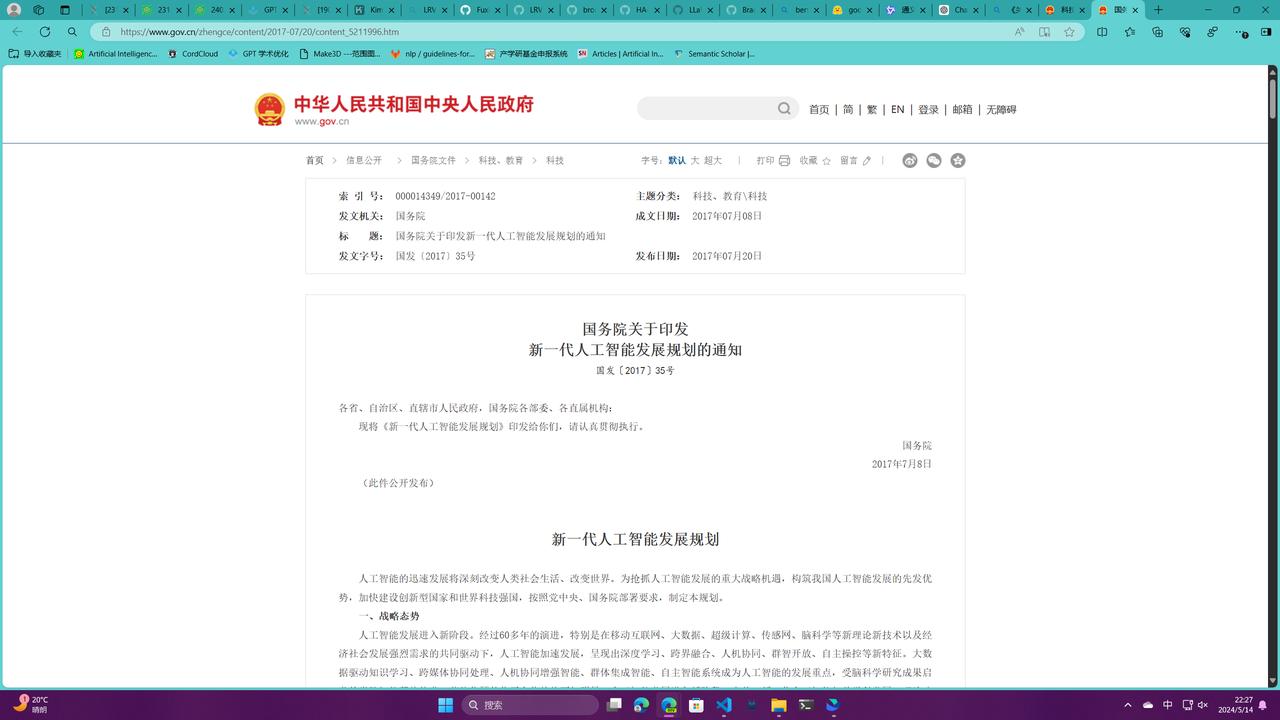
\includegraphics{images/policy_1.PNG}
\end{marginfigure}
中国政府2017年制定的《新⼀代⼈⼯智能发展规划》中提出了到2030年成为世界主要人工智能创新中心的目标,充分体现了中国对AI发展的高度重视和积极支持。在科技部等部门2022年联合印发的《关于加快场景创新以人工智能高水平应用促进经济高质量发展的指导意见》中,也提出了鼓励通过场景创新推动AI技术的应用,促进经济的高质量发展的意见。

\begin{marginfigure}
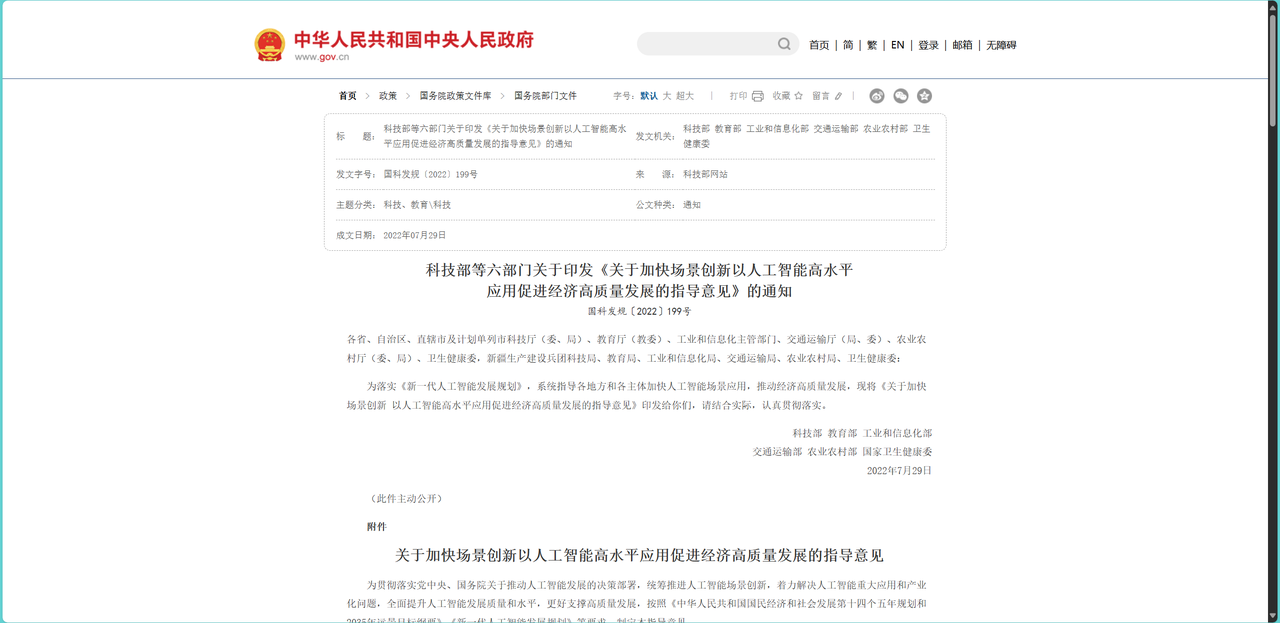
\includegraphics{images/policy_2.PNG}
\end{marginfigure}
在大力支持人工智能发展的同时,相关政策法规也非常关注对人工智能发展进行必要的约束。例如,《中华人民共和国个人信息保护法》即围绕个人信息的处理,确立了处理规则、跨境提供、个人权力、处理者义务等方面的规则,对AI技术在数据收集和处理方面的应用提供了法律约束。2021年出台的《新一代人工智能伦理规范》则针对AI发展提出了增进人类福祉、保护隐私安全、确保可控可信等基本伦理要求,并对特定活动提出了具体的伦理要求。

\subsection{管理与限制}
同时,国内外立法和行业管理机构也非常重视引导AI技术的发展和管控风险。

在欧盟委员会提出的《人工智能法案》中,在建立统一的AI技术规则时,重点强调了风险管理和伦理标准,并对高风险AI技术规定了与之匹配的监管等级。我国在《新⼀代⼈⼯智能发展规划》中,制定了促进AI发展的法律法规和伦理规范,建立了人工智能法律主体及相关权利、义务和责任框架,针对AI可能带来的社会、伦理和法律问题,制定相应的政策措施。

在风险管控方面,我国在《关于加快场景创新以人工智能高水平应用促进经济高质量发展的指导意见》中,努力建立健全公开透明的AI监管体系,实行设计问责和应用监督并重的双层监管结构。欧盟的《人工智能法案》引入了风险分级监管、市场准入制度、监管沙盒等制度;美国政府提出的《人工智能权利法案蓝图》,则为AI系统设立了五项基本原则,包括数据隐私、算法歧视保护等,旨在保护人权并推动AI技术的健康发展。

\section{法律之网}

\subsection{引言}
AI技术的发展为法律领域带来了新的挑战和机遇。一方面,AI的应用可以提高法律服务的效率和质量,例如通过自动化的法律咨询、案例分析和文档审查等。另一方面,AI技术的复杂性和自主性也引发了法律和伦理问题,如数据隐私、算法歧视、责任归属等,这些问题需要法律专家和立法机构制定相应的法规和政策来解决。同时,AI的发展也促使法律体系不断更新,以适应技术变革带来的新情况。法律需要明确AI的权利和责任界限,确保技术的合理使用,并保护个人和社会的利益。因此,AI与法律之间的关系是动态发展的,需要持续的对话和合作,以实现科技与法律的和谐共存。

\subsection{AI系统的法律责任}

AI系统中法律责任的界定问题是一个复杂且不断发展的领域。随着自主决策系统的普及和能力的提升,AI的行为可能引发法律纠纷,这要求法律体系能够适应新技术带来的挑战。

首先,当AI系统的行为引发法律纠纷时,传统的侵权责任法原则可能需要调整以适应AI的特殊性。根据现有的法律框架,AI本身通常不被认为具有法律责任主体的地位,因为它们缺乏承担责任所需的财产,并且不能具有人类的主观意图或过错。因此,责任通常归属于与AI系统的设计、开发、生产、销售或使用相关的个人或实体。

在判定责任时,法院可能需要考虑多个因素,包括但不限于:

1. 设计缺陷:如果AI系统的设计存在缺陷,导致了损害的发生,设计者可能需要承担责任。
2. 生产缺陷:如果AI系统在生产过程中出现缺陷,生产者可能需要承担责任。
3. 使用不当:如果AI系统的使用者未能正确使用系统,导致了损害,使用者可能需要承担责任。
为了提高法律责任的明确性和可追溯性,以下是一些建议:
4. 透明度和可解释性:AI系统应当设计为能够提供关于其决策过程的透明和可解释的信息,这有助于确定责任归属。
5. 记录和审计:应要求AI系统的开发者和使用者记录和保存系统的操作日志和决策数据,以便在发生纠纷时进行审计和分析。
6. 法律和伦理准则:制定和实施针对AI系统的法律和伦理准则,明确AI系统的行为标准和责任主体的义务。
7. 保险和风险管理:鼓励或要求AI系统的开发者和使用者购买责任保险,以减轻潜在的财务损失,并推动风险管理的最佳实践。
8. 持续的法律研究和改革:随着AI技术的发展,法律体系需要不断更新和改革,以确保责任判定能够适应新的技术现实。


\begin{table*}[htbp]
\centering
\begin{tabular}{p{4cm}|p{4cm}|p{4cm}}
\hline
因素 & 考虑内容 & 相关建议 \\
\hline
设计缺陷 & AI系统设计缺陷 & 设计者可能需承担责任。 \\
\hline
生产缺陷 & AI系统生产过程缺陷 &  生产者可能需承担责任。 \\
\hline
使用不当 & AI系统使用者未正确使用 &  使用者可能需承担责任。 \\
\hline
透明度和可解释性 & AI系统决策过程透明可解释性 &  提供决策过程的透明信息。 \\
\hline
记录和审计 & 记录和保存系统操作日志和决策数据 &  进行审计和分析。 \\
\hline
法律和伦理准则 & 针对AI系统的法律和伦理准则 &  明确行为标准和责任主体义务。 \\
\hline
保险和风险管理 & 责任保险和风险管理实践 &鼓励或要求购买责任保险,减轻财务损失。 \\
\hline
持续的法律研究和改革 & 适应新技术现实的法律改革 & 持续更新法律体系。 \\
\hline
\end{tabular}
\caption{AI系统责任相关因素表}
\label{tab:ai_factors}
\end{table*}

AI系统引发法律纠纷时的责任判定需要综合考虑多个因素,并且需要法律体系、技术开发者和使用者共同努力,以确保责任的明确性和可追溯性。随着AI技术的不断进步,法律制度也必须适应新的挑战,确保公平和正义得到维护。

\subsection{AI技术与隐私}

AI技术对隐私法律提出了重大挑战,特别是在个人数据收集、处理和共享方面。AI系统为了实现智能化功能,通常需要大量的数据输入,这包括个人身份信息、行为习惯、位置数据等敏感信息。这些数据的收集和使用如果没有得到适当的管理和保护,就可能侵犯个人隐私权。

在法律框架下,个人数据的收集和处理受到严格的规范。例如,欧盟的《通用数据保护条例》(GDPR)规定了数据最小化、目的限制、数据准确性、透明性等原则,要求数据控制者在处理个人数据时必须遵守。此外,数据主体拥有知情权、访问权、更正权、删除权等,以保护其个人隐私不受侵犯。

然而,AI技术的发展往往需要跨领域、跨平台的数据整合和分析,这与现有的隐私法律框架存在冲突。为了平衡科技创新和隐私权的冲突,以下是一些可能的措施:

1. 强化数据保护法规:更新和完善隐私法律,确保法规能够适应AI技术的发展,同时保护个人隐私权。例如,可以引入数据保护影响评估(DPIA)等机制,对AI系统的数据使用进行预先评估。
2. 促进技术创新与合规性:鼓励AI开发者采用隐私增强技术(PETs),如匿名化、去标识化等,以减少对个人隐私的依赖。同时,推动建立行业标准和最佳实践,引导AI技术的合规发展。
3. 提高透明度和控制权:确保用户能够了解其数据如何被收集和使用,并提供足够的控制权,让用户能够决定自己的数据是否被用于AI分析。
4. 加强监管和执法:监管机构应加强对AI数据处理活动的监督,确保企业遵守隐私法规。对于违反隐私法律的行为,应采取有效的执法措施,包括罚款和制裁。
5. 公众教育和意识提升:通过教育和宣传活动,提高公众对个人数据隐私的认识,使他们能够更好地保护自己的隐私权益。

显然,平衡科技创新和隐私权的冲突需要多方面的努力,包括法律制定者、技术开发者、企业和用户等各方的参与和合作。只有制定合理的法规、采用创新的技术解决方案、加强监管和提高公众意识,我们才可以在保护个人隐私的同时,促进AI技术的健康发展。

\subsection{透明度与可解释性的法律规定}

法律对AI系统的透明度和可解释性的要求是为了确保AI系统的决策过程能够被解释和审查,满足法律的规制和伦理的要求。

各国政府已经开始立法对AI系统的透明度和可解释性加以规范,以确保用户和监管机构能够理解AI系统的决策过程。例如,欧盟的《通用数据保护条例》(GDPR)要求,在完全自动化的决策过程中,数据主体有权获得决策逻辑的解释。我国的《个人信息保护法》也提出了类似的要求,强调算法自动化决策的透明度和结果的公平、公正。

AI系统的“黑箱”特性使得其决策过程难以解释。为了提高可解释性,研究者和开发者正在探索各种技术手段,如可解释的人工智能(XAI)和算法说明书机制。这些技术旨在提供关于AI决策过程的清晰和有意义的信息,以便用户和监管机构能够进行有效的审查。

伦理原则和法律规制的结合也是提高AI系统透明度和可解释性的关键。例如,我国的《新一代人工智能伦理规范》提出了保护隐私安全、确保可控可信等伦理规范。欧盟的《人工智能法案》也旨在建立一套统一的规范和监管框架,确保AI技术的发展和应用能够遵循公平、透明和可信的原则。

尽管法律和伦理原则提供了指导,但在实践中确保AI系统的透明度和可解释性仍面临挑战。与欧美相比,目前中国的算法治理规则比较分散,缺乏实施的细则和操作指引。为了应对这些挑战,建议采取包容审慎的立场,建立分级分类分场景的监管方式,同时借鉴食品营养成分表等信息披露机制,为符合条件的AI系统建立“算法说明书”机制。

确保AI系统的透明度和可解释性是满足法律要求的关键。这需要法律、技术、伦理和市场力量的共同作用,通过制定合理的法规要求、开发有效的技术解决方案、建立伦理审查机制,并在实践中不断调整和完善相关政策和措施。通过这些努力,可以增进用户对AI系统的信任,防范算法歧视,支持内部治理,并促进人机协作。

 
\subsection{国际合作与法规规定}

国际人工智能公司(例如OpenAI)在遵守不同国家法规时面临的法律挑战主要包括以下几点:

1. 多元法律体系的适应性:跨国公司的业务活动跨越多个司法管辖区,需要遵守各国独立的法律制度和法规框架。不同国家的法律体系差异巨大,这对公司构成了适应性的挑战,要求公司必须熟悉并遵守各国的法律法规,以避免法律风险和罚款。
2. 合规监管的复杂性:跨国公司不仅要遵守所在国的法律法规,还需要考虑国际组织的要求,如世界贸易组织(WTO)、经济合作与发展组织(OECD)等的相关规定。这些监管框架的复杂性使得合规工作变得更加困难。
3. 国际法规协调的努力:当前,国际组织和协定正在努力协调跨境人工智能法规。例如,OECD建立了全球人工智能合作伙伴关系框架,旨在促进国际间的合作与对话,推动形成共同的人工智能治理原则和标准。
4. 国际合作机制的需求:为了应对上述挑战,法规制定中可能需要的国际合作机制包括:
  - 建立国际标准:通过国际标准化组织等机构制定统一的技术标准和规范,降低跨国公司在不同国家运营的合规成本。
  - 促进信息共享:建立国际平台,促进各国监管机构之间的信息共享,提高监管效率和透明度。
  - 共同监管框架:制定跨国界的共同监管框架,为人工智能等新兴技术提供一致的法律指导和监管要求。
  - 国际争端解决机制:设立专门的国际争端解决机构,处理跨国公司在遵守不同国家法规时出现的法律争端。
 
通过这些国际合作机制,可以促进全球法规的一致性和协调性,帮助跨国公司更有效地应对不同国家的法律挑战,同时也有助于保护消费者权益和促进公平竞争。
 

\subsection{法官培训与技术审查}
法官和法律专业人士在处理人工智能相关案件时面临的法律认知问题主要包括对人工智能技术的理解和评估、算法决策的透明度和可解释性、以及技术性证据的审查等方面。

1. 对人工智能技术的理解和评估:法官在裁判过程中需要对涉及人工智能技术的案件进行评估,这要求他们具备一定的技术知识。然而,人工智能技术的复杂性和专业性可能导致法官在理解和评估相关技术时遇到困难,从而影响案件的公正裁决。

2. 算法决策的透明度和可解释性:人工智能系统尤其是那些基于机器学习的系统,往往被视为“黑箱”,其决策过程缺乏透明度。法官在审理案件时,需要能够理解和解释算法决策的逻辑,以确保裁判的公正性和合理性。

3. 技术性证据的审查:随着技术性证据在案件中的重要性日益增加,法官和法律专业人士需要具备审查这些证据的能力。这包括对电子数据、算法生成的报告等技术性证据的真实性、合法性和相关性的评估。

为了更好地处理这些问题,可能需要对法官进行专门的培训,以提高他们对人工智能技术的理解,并培养他们在技术性证据审查方面的能力。这种培训可以包括:

1. 技术知识教育:通过培训,法官可以了解人工智能的基本原理、常见应用以及可能的法律问题。
2. 案例分析:通过分析涉及人工智能的具体案例,法官可以更好地理解技术如何在司法实践中应用。
3. 实践操作:提供模拟操作环境,让法官亲身体验人工智能系统的工作流程,增强对技术的直观理解。

法律系统整合技术审查机制的方法可能包括:

1. 建立专家咨询制度:聘请技术专家作为顾问,为法官提供专业的技术意见。
2. 设立专门的技术审查团队:组建由技术专家组成的团队,专门负责审查技术性证据。
3. 完善技术性证据审查制度:制定明确的技术性证据审查标准和流程,确保审查工作的规范性和有效性。

总之,随着人工智能技术在司法领域的应用日益广泛,法官和法律专业人士需要通过专门的培训和法律系统的技术整合,提升对人工智能相关案件的处理能力,确保司法公正和技术发展的和谐统一。

\subsection{法规的灵活性与科技创新}
法律法规的制定对AI技术的发展和应用至关重要,因此需要不断评估现有法律法规的适用性,尤其是是否足以适应不断变化的AI技术。人工智能技术日新月异,新技术和应用不断涌现,相关法规必须足够灵活,才能及时适应技术的变革,确保法规的相关性和有效性。同时,法规的灵活性更可以鼓励企业和研究机构进行创新尝试,避免因法规僵化而抑制科技创新和产业发展。

另一方面,在面对人工智能技术可能带来的隐私、安全等方面的风险时,灵活的法规能够更好地应对这些风险,保护公众利益和社会稳定。尤其是面对人工智能技术的发展带来的伦理和道德风险时,灵活的法规能够更好地融入伦理道德考量,引导技术发展符合社会价值和伦理标准。

法规的灵活性可以帮助公众建立对人工智能技术的信任,通过合理的监管措施,让公众相信技术的发展是在可控和有序的框架下进行的。是当人工智能技术与其他领域如医疗、交通、教育等融合时,更需要法规能够灵活适应不同领域的特殊需求和挑战。而随着全球人工智能竞争的加剧,灵活的法规在吸引国际投资和顶尖人才进而提升国家在全球市场中的竞争力方面,其作用亦不可小觑。

对现有人工智能法规的灵活性评估需要从多个角度进行考量。从法规制定的速度来看,随着人工智能技术的快速发展,法规的更新和制定必须能够及时跟进技术的步伐。

为了在法规中融入灵活性以促进科技创新,可以采取以下几个策略:

1. 动态监管机制:建议建立动态的人工智能分级分类监管机制,通过区分关键人工智能和一般人工智能,避免“一刀切”的监管,这样可以根据不同技术的特点和发展阶段,实施更为精准和适应性强的监管策略。

2. 预留接口与灵活条款:法规应为未来可能出现的新技术和应用场景预留足够的接口,例如在知识产权问题上留出调整空间,允许法规在未来根据技术发展进行适应性调整。

3. 公众参与和透明度:增加公众参与度,通过征求意见、公众听证会等方式,让法规制定过程更加透明,同时确保公众对新技术的理解和关切能够被立法者听取和考虑。

4. 风险评估与管理:强调基于风险的监管方法,对不同风险级别的人工智能应用采取不同的管理措施,确保监管措施与技术发展的风险相匹配。

5. 国际合作与标准制定:积极参与国际规则和标准的制定,推动国际间的规则互认,以便国内法规能够与国际标准保持一致,促进技术的国际交流和合作。

6. 促进发展创新原则:在法规中明确提出鼓励人工智能研发和应用,支持基础设施建设,推动公共资源的开放共享,创新探索适应人工智能发展的知识产权制度。

通过上述策略,法规可以更好地适应技术的快速发展,同时为科技创新提供支持和空间。这要求立法者、监管者和技术开发者之间建立紧密的沟通和协作机制,确保法规既能够保护公共利益,又能够促进技术的健康发展。另一方面,考虑到人工智能技术的发展速度可能会超过了现有法规制定的速度,特别是在应用场景和商业模式尚不明朗的探索阶段,立法时机可能尚未成熟,过早的立法可能会限制技术创新,所以,对立法时机的选择也需要高度灵活,要不疾不徐。

\subsection{未来的法律框架}
未来人工智能(AI)治理法规的法律框架需要适应技术发展的趋势和特点,同时也要考虑到社会、伦理和安全等多方面的需求,应是一个多元化、动态化、国际化和人性化的体系,可以有效平衡技术创新与社会责任,确保AI技术的健康、安全和可持续发展。

1. 强化伦理原则:随着AI技术的发展,法律框架将更加重视伦理原则的融入,确保AI的发展符合人类的伦理道德标准。例如,应强调AI应用的公平性、透明性和可解释性,以及对个人隐私的保护。
2. 动态监管机制:法律框架将采用更加灵活的监管机制,以适应AI技术的快速发展。这可能包括定期审查和更新法规,以及建立快速响应机制来处理新出现的技术和社会问题。
3. 跨部门协作:AI技术的应用涉及多个领域,因此法律框架鼓励和规范跨部门协作,确保不同领域的法规能够相互衔接,形成统一协调的治理体系。
4. 公众参与:未来的法律框架应更加注重公众参与,通过公开征求意见、举行听证会等方式,让公众对AI治理法规的制定有更多的发言权和参与度。
5. 国际合作:鉴于AI技术的全球性特征,法律框架应强调国际合作的重要性,参与国际标准的制定,推动国际间的法规互认和协调。
6. 促进创新与防范风险并重:法律框架应在促进技术创新和产业发展的同时,加强对潜在风险的预防和控制,确保AI技术的安全可控。
7. 明确责任归属:随着AI系统自主性的提高,法律框架应明确AI系统及其开发者、使用者的责任归属,确保在发生问题时能够追溯并追究责任。
8. 技术中立性原则:法律框架应尽可能保持技术中立,避免对特定技术或应用领域产生不公平的偏见或限制,同时为新技术的发展留出空间。
9. 强化数据治理:数据是AI技术的基础,法律框架应加强对数据收集、处理和使用的规范,确保数据安全和合规使用。
10. 人工智能教育和培训:法律框架应鼓励和规范AI相关的教育和培训,提高公众和专业人员的AI素养,促进社会的适应和接受。

综上,未来的人工智能治理法律法规应当具备足够的创新性和适应性,以保障其能够跟上AI技术的快速发展,并有效应对由此带来的挑战。法律法规应适时修订、动态更新;应保持技术中立;应进行分级分类监管,根据人工智能系统的风险等级和应用领域进行差异化管理;应明确伦理原则,在公平性、透明性、可解释性以及隐私保护等方面提升公众对AI技术的信任和接受度。从根本上,未来的法律法规应能促进产业发展与创新,在制定过程中应增加公众参与度,让法规制定过程更加透明,确保法律法规的公平、合理、适用,能够成为社会和谐进步的助推剂和稳定剂。

% % \setchapterstyle{kao}
\setchapterimage[6.5cm]{ethics_2}
\setchapterpreamble[u]{\margintoc}
\chapter[人工智能伦理与安全 - 对话与思考]{人工智能伦理与安全 - 对话与思考 \footnotemark[0]}

\footnotetext{The credits for the image above the chapter title go to:
	Image generated by OpenAI's DALL-E, used in accordance with OpenAI's terms and conditions.}
 
\section{数据隐私}

在互联网长期发展的过程中,我们见证了许多个人隐私数据的泄露和滥用。一个突出的例子是“人肉搜索”,这是一种利用搜索引擎等工具来追踪、收集和公开他人信息的行为,导致了许多不幸事件的发生,如个人隐私暴露、人身安全受到威胁等。在这种情况下,一些知名的科技公司和互联网平台开始意识到数据隐私和安全的重要性。作为其中之一的谷歌,它曾经将自己的口号改为“Don't be evil”(不作恶),强调了对道德和社会责任的承诺。然而,由于一些不良行为和事件的出现,包括个人隐私数据的滥用和泄露,谷歌在一段时间后将口号修改为“Do the right thing”(做正确的事),以更加准确地表达其对道德和合规的追求。

上述例子提醒着我们,保护个人隐私数据和确保其安全是科技公司和互联网平台应当重视的责任。随着人工智能时代的来临,相关技术已经深入到了我们生活的方方面面,数据隐私和安全问题开始变得愈发紧迫和重要。2017年,我国颁布的《中华人民共和国网络安全法》也强调了对个人隐私信息的保护。因此,如何充分防范人工智能技术应用中的数据泄露风险,已经成为该技术进一步发展与部署不得不面临的问题之一。

当前,人工智能的核心技术主要是基于深度学习的神经网络,该技术在训练模型时通常需要使用大规模的数据集,而这些数据往往来自互联网上的公开数据,例如,自然语言处理领域中的BERT以及ChatGPT使用了大规模的语言数据集,计算机视觉领域的ImageNet数据集也是通过收集互联网上的图像得到的。然而,这些公开数据中可能存在大量的个人隐私信息。如果这些数据被直接用来训练模型,就存在个人隐私数据的泄漏风险,从而给个人和社会带来潜在的危害。因此,我们有必要采取措施来确保在人工智能的发展和应用过程中保护个人隐私数据的安全性和保密性。

互联网上蕴含的海量数据,这是人工智能的基石,如果不能使用这些数据,则人工智能将无从谈起。因此,数据还是得要使用,但是在使用数据训练模型时需要采取一系列的措施来保护数据安全,包括但不限于数据加密、访问控制、数据匿名化和脱敏等。同时,我们还需要建立严格的数据保护和隐私政策,制定明确的数据使用规则,确保数据的合法、合规和道德使用。

除了技术手段外,教育和意识提升也是至关重要的。我们需要加强对数据隐私和安全的宣传和教育,提高公众的意识和保护个人隐私的意识。只有通过技术手段和社会共识的双重保障,我们才能够最大程度地降低数据泄露和隐私风险,保护个人和社会的权益,推动人工智能技术的健康发展。

\section{模型安全}

当前,互联网上涌现了大量形形色色的人工智能模型和服务,有的模型开发者选择直接开源他们的模型使得其在全球范围内得以广泛应用,从而促进相关研究的进一步发展,例如huggingface;而另外一些模型开发者选择封闭他们的模型并提供服务的接口给用户使用,例如chatgpt。

近年来,探索攻击人工智能模型的相关研究愈发引人关注。无论是模型的开源与否,都存在着被破坏数据隐私与安全的风险。

1. 首先,开源模型的广泛普及使得模型的代码和参数对于任何人都是可见的。虽然这种开放性促进了合作和创新,但同时也使得破坏这类模型的数据隐私与安全变得更加容易。攻击这类模型的相关研究被称为白盒攻击,通过一些技术手段可以获取模型的训练数据,从而窃取用户的隐私信息。

2. 其次,封闭模型虽然限制了模型参数的可见性,但也并非完全安全。一些攻击者可以利用模型提供的服务接口进行攻击,通过恶意数据来诱导模型泄露敏感信息。这种类型的攻击被称为黑盒攻击,攻击者虽然无法直接访问模型的内部结构,但可以通过测试不同的输入来推断模型的行为,并尝试找到模型的弱点,从而获取敏感信息。

上述攻击行为不仅严重威胁个人隐私安全,也可能对社会造成严重的危害。从技术难度上来看,黑盒攻击要比白盒攻击困难得多。白盒攻击能够直接访问模型的内部结构,因此攻击者可以更容易地获取训练数据和模型参数,从而窃取用户的隐私信息。而黑盒攻击则需要通过间接的方法来推断模型的行为,攻击者无法直接访问模型的内部结构,因此技术上的难度更高。接下来将分别就白盒攻击和黑盒攻击来探讨相应的可行解决方案。

对于白盒攻击来说,由于攻击者能够直接访问模型的内部结构和参数,因此其攻击难度较低,开放的模型无法阻止模型的行为,从而使得防范白盒攻击变得困难。但是随着科学技术的发展,目前已经出现了一些技术手段来防止白盒攻击的发生。

1. 一种常见的方法是在模型训练阶段对训练数据进行预处理,消除其中蕴含的隐私信息。例如,可以使用数据脱敏技术或者隐私保护算法对训练数据进行处理,以降低训练数据中蕴涵的隐私信息比例;

2. 另一种方法是通过给训练模型的损失函数增加一些正则化约束,防止参数直接泄露训练数据。例如,可以引入差分隐私机制或者添加模型参数的噪声,是的攻击者无法通过模型参数推断出模型的训练数据。

虽然上述技术手段能够有效防止白盒攻击的发生,但是也会带来一些负面影响。例如,可能导致模型的性能下降,因为数据预处理或者添加正则化约束可能会降低模型的训练效果。此外,这些技术手段可能会增加模型训练的复杂度和工作量,导致训练过程更加耗时和昂贵。

事实上,还有一种方法就是将模型闭源,使得使用者只能通过接口来访问人工智能模型提供的服务。通过这种方式,攻击者想要窃取模型的数据隐私,则只能通过黑盒攻击的方式,而黑盒攻击相对于白盒攻击来说难度更高,因为攻击者无法直接访问模型的内部结构和参数。这样做可以提高攻击的门槛,从而有效地避免了大量可能的数据隐私与安全问题。然而,闭源模型可能会限制相关技术的发展,由于模型的内部结构和参数对外不可见,其他研究者和开发者无法对其进行深入的研究和探索,这可能会阻碍了新技术的创新和发展,限制人工智能技术的进一步发展。

关于人工智能模型的开源与否是人工智能领域的一个长期话题,OpenAI作为世界领先的人工智能实验室之一,早期的使命是创造出人类水平甚至超越人类水平的通用人工智能(AGI),并且希望将其利益平均分配给全世界。然而,随着人工智能技术的不断发展和应用,对于人工智能模型可能被恶意利用的担忧也日益增加。特别是在GPT-2模型发布之后,OpenAI决定不公开其源代码,而是选择通过API的方式提供对该模型的访问权限,以限制模型被滥用的可能性。这一决定引发了社会各界的热议,一方面有人认为这是为了保护公众免受潜在的伤害,另一方面也有人担心这种做法可能阻碍了人工智能技术的开发和创新,以及对模型的透明度和可信度提出了质疑。

类似的情况也出现在后续推出的爆火的ChatGPT模型上,其源代码也未公开。这种做法引发了一些争议,因为一些人认为开源对于促进技术的发展和透明度至关重要,而另一些人则认为保护模型的安全和防止滥用同样重要。

因此,人工智能模型的开源与否确实是一个长期的话题,需要在技术创新、商业利益、安全性和社会责任等多方面进行权衡,以找到最合适的解决方案。这也反映了人工智能领域所面临的伦理和社会问题,需要在不断探索和实践中寻找平衡点。

\section{应用规范}

人工智能的发展经历了从判别式神经网络到生成式神经网络的重大变革。在早期,判别式神经网络主要用于解决分类和识别任务,如图像分类、语音识别等。这种网络通过学习从输入数据到标签或类别的映射关系来对数据进行分类。

然而,随着生成式神经网络的研究不断深入,人工智能开始具备了生成能力,这是一场革命性的转变。生成式神经网络能够从学习数据的分布中直接生成新的数据样本,而不仅仅是对已有数据进行分类或识别。这种能力使得人工智能系统能够创造出新的、以前从未见过的内容,从而展示了更高级的智能和创造性。

正如著名科学家费曼的名言所说,“what I cannot create, I do not understand.”,高水平的生成式人工智能的出现,标志着人工智能已经能够深入理解数据的本质和内在规律。长期以来,创造力被认为是人类的专属领域,是人工智能难以企及的差距。然而,随着人工智能技术的飞速发展,特别是以ChatGPT、MIdjorney等为代表的AIGC(Artificial Intelligence Generative Content)软件的出现,这一传统观念正在发生改变。这些AI生成内容的软件已经逐渐渗透到我们生活的各个方面,从文字创作到音乐、绘画、甚至影视剧本的创作,都有着不同程度的应用。

这些AI生成内容的软件正在重新塑造内容创作的布局。它们能够在短时间内生成大量的内容,从而帮助人们提高生产效率,解放创作者的思维和时间,同时也为那些缺乏创作能力或经验的人提供了创作的机会。然而,这种技术的应用也带来了一些问题和挑战:

1. 原创性和版权问题:人工智能生成的内容可能引发原创性和版权方面的争议。由于人工智能模型在训练时会使用互联网上的大量数据,其中可能包含他人的原创作品。因此当模型在生成内容时,很难确定其是否与已有作品相似或者涉嫌抄袭他人的创意,甚至这些内容会直接和他人的原创作品完全一致。这种情况对于版权持有人来说是一个挑战,因为他们的作品可能被人工智能模型直接使用,而无法获得适当的授权或报酬。同时,对于人工智能生成内容的使用者来说,也可能面临法律风险,因为他们可能会被指控侵犯了他人的版权。解决这一问题的关键在于建立更加清晰的法律框架和准确的判定标准,以便界定AI生成内容的原创性和版权归属。

2. 道德和伦理问题: 人工智能只是一个数字系统,没有人类的情感和道德判断能力,因此其生成的内容可能存在一些潜在的风险和问题,从而可能会对产生不良影响。因此,需要对生成的内容进行审查和管理,以确保其符合道德和伦理标准。这需要建立一套全面的审核机制,确保AI生成的内容符合社会公共利益和道德底线。

3. 品质和可信度问题:尽管人工智能可以在短时间内生成大量的内容,但并不意味着这些内容都具有高质量和可信度。AI生成的内容通常是基于已有的数据模型,可能存在一些错误或不准确的信息。这种问题被称为人工智能的幻觉问题,即人们可能错误地认为AI生成的内容是准确和可信的。虽然已经有大量的研究人员发现了该问题,并且尝试进行解决,但目前还没有一个完美的解决方案。因此,需要进行后续的审核和编辑以提高内容的品质和可信度。这可能需要引入人工审核和编辑,以确保内容的准确性和可靠性。

4. 人工智能的滥用问题:人工智能生成的内容可能被用于恶意目的,如散播虚假信息、诱导观众或操纵舆论等。为了防止人工智能技术的滥用,需要采取措施来加强技术监管和法律规范,建立健全的信息安全体系,提高公众对虚假信息的辨识能力,以减少不良影响。这也需要平台和相关机构加强监管和管理,及时发现并阻止任何恶意行为的发生。

尽管人工智能在内容创作领域的应用带来了新的可能性和机遇,但仍然需要人类创作者的参与和监督,以确保内容的质量和意义。人类创作者可以与人工智能技术相结合,发挥各自的优势,共同创造出更加丰富、有价值的作品,从而推动内容创作领域的进步和发展。

\section{结语}

在过去若干年内,强人工智能一度被认为是一个遥不可及的目标。这是因为要实现强人工智能,人工智能系统需要具备像人类一样的智能、自我意识和通用推理能力。然而,随着深度学习技术的不断发展,强人工智能似乎变得更加可能了。

以ChatGPT为代表的对话机器人能够理解人类的文字并输出相应的文字回复,可以轻松通过“图灵测试”,这为人机交互的进步带来了新的可能性。同时,视觉模型结合摄像头使得机器能够看到和理解周围的环境,为自主导航和环境感知提供了技术基础。语音模型的发展使得理解和合成人类的语音成为可能,为人机交互提供了更加直观和自然的方式。此外,机器人技术的进步,例如机器手臂的发展,使得机器能够执行各种物理任务,从而拓展了其应用领域。

随着我们逐步迈向强人工智能时代,我们需要认真思考和解决相关的伦理和社会问题,以确保人工智能技术能够为人类带来真正的价值和益处,而不是给人类带来不可磨灭的伤害。关于人工智能技术的监管准则最早可以追溯到1942年,阿西莫夫的科幻作品《我,机器人》中提出的机器人学三定律:

1. 第一定律:机器人不得伤害人类,也不得因不作为而使人类受到伤害。
2. 第二定律:机器人必须服从人类的命令,除非这种命令与第一定律相冲突。
3. 第三定律:机器人必须保护自己的存在,但前提是不违反第一定律和第二定律。

尽管这些定律为我们提供了一个基本的伦理框架,但随着技术的发展,它们已经显露出一定的局限性。特别是,人工智能系统可能面临的复杂情况和伦理挑战超出了这三个简单的准则所能涵盖的范围。因此,科学家和政策制定者们正在努力制定更为全面和具体的人工智能伦理准则和监管政策。这些准则可能包括对数据隐私的保护、算法的公平性和透明度、机器人责任和道德规范等方面的规定。此外,国际社会也在探讨建立全球性的人工智能治理机制,以促进跨国合作和信息共享,共同应对人工智能带来的伦理和社会挑战。

尽管人工智能技术的发展道路上还面临着诸多的挑战和风险,但我们不应该因为困难而止步不前。技术的本质是为了促进生产力的提升,让人类能够过上更加美好的生活。因此,我们需要积极地应对这些挑战和风险,并不断地探索和创新,发挥人工智能技术的潜力,为人类社会的进步和发展做出更大的贡献。最后,让我们共同拥抱人工智能时代的来临!通过不懈的努力和创新,我们可以共同开创一个更加智能、更加美好的未来。


% \appendix % From here onwards, chapters are numbered with letters, as is the appendix convention

% \pagelayout{wide} % No margins
% \addpart{附\ 录}
% \pagelayout{margin} % Restore margins

% \input{chapters/appendix.tex}

%----------------------------------------------------------------------------------------

\backmatter % Denotes the end of the main document content

\setchapterstyle{plain} % Output plain chapters from this point onwards

%----------------------------------------------------------------------------------------
%       BIBLIOGRAPHY
%----------------------------------------------------------------------------------------

% % The bibliography needs to be compiled on the command line with 'biber main' from the template directory

\defbibnote{bibnote}{Here are the references in citation order.\par\bigskip} % Prepend this text to the bibliography
\printbibliography[heading=bibintoc, title=参考文献, prenote=bibnote] % Add the bibliography heading to the ToC and set the title of the bibliography

%----------------------------------------------------------------------------------------
%       INDEX
%----------------------------------------------------------------------------------------

% The index needs to be compiled on the command line with 'makeindex main' from the template directory

\printindex % Output the index

%----------------------------------------------------------------------------------------
%       BACK COVER
%----------------------------------------------------------------------------------------

% If you have a PDF file that you want to use as back cover, uncomment the following lines.

%\clearpage
%\thispagestyle{empty}
%\null%
%\clearpage
%\includepdf{cover-back.pdf}

%----------------------------------------------------------------------------------------

\end{document}

%%% Local Variables:
%%% mode: latex
%%% TeX-master: t
%%% End:
